\documentclass[conference]{IEEEtran}
\IEEEoverridecommandlockouts
% The preceding line is only needed to identify funding in the first footnote. If that is unneeded, please comment it out.
\usepackage{cite}
\usepackage{amsmath,amssymb,amsfonts}
\usepackage{algorithmic}
\usepackage{graphicx}
\usepackage{textcomp}
\usepackage{xcolor}


\usepackage{listings}   % Required for the listings package

% Define custom FXML language
\lstdefinelanguage{FXML}{
    morekeywords={AnchorPane, VBox, ImageView, Label, Button, fx:id, xmlns, fx:controller, onAction},
    sensitive=true, % Case-sensitive
    morecomment=[s]{<!--}{-->}, % XML-style comments
    morestring=[b]" % Strings in double quotes
}

\lstset{
    language=FXML,
    basicstyle=\ttfamily\small, % Monospaced font
    keywordstyle=\color{blue}\bfseries, % Style for keywords
    commentstyle=\color{green}, % Style for comments
    stringstyle=\color{red}, % Style for strings
    numbers=left, % Line numbers
    numberstyle=\tiny, % Small line numbers
    frame=single, % Frame around the code
    breaklines=true % Wrap long lines
}

% Configure the listings package
\lstset{
    basicstyle=\ttfamily\small, % Use monospaced font and small size
    keywordstyle=\color{blue}\bfseries, % Style for keywords
    commentstyle=\color{green}, % Style for comments
    stringstyle=\color{red}, % Style for strings
    numbers=left, % Line numbers on the left
    numberstyle=\tiny, % Tiny line numbers
    breaklines=true, % Wrap long lines
    frame=single % Single frame around the code
}

\usepackage{hyperref}

\def\BibTeX{{\rm B\kern-.05em{\sc i\kern-.025em b}\kern-.08em
    T\kern-.1667em\lower.7ex\hbox{E}\kern-.125emX}}
\begin{document}

\title{Hick Hack in Gackelwack\\
% {\footnotesize \textsuperscript{*}Note: Sub-titles are not captured in Xplore and
% should not be used}
%\thanks{Identify applicable funding agency here. If none, delete this.}
}

\author{\IEEEauthorblockN{Khoi Nguyen Nguyen}
\IEEEauthorblockA{\textit{Bachelor of Informatik} \\
% \textit{name of organization (of Aff.)}\\
Ho Chi Minh, Vietnam \\
khoi.nguyen@stud.fra-uas.de}
\and
\IEEEauthorblockN{Tran Quoc Dat Nguyen}
\IEEEauthorblockA{\textit{Bachelor of Informatik} \\
% \textit{name of organization (of Aff.)}\\
Ho Chi Minh, Vietnam \\
dat.nguyen-tran-quoc@stud.fra-uas.de}
\and
\IEEEauthorblockN{Duc Minh Khoa Ngo}
\IEEEauthorblockA{\textit{Bachelor of Informatik} \\
% \textit{name of organization (of Aff.)}\\
Ho Chi Minh, Vietnam \\
duc.ngo@stud.fra-uas.de}
% \and
% \IEEEauthorblockN{4\textsuperscript{th} Given Name Surname}
% \IEEEauthorblockA{\textit{dept. name of organization (of Aff.)} \\
% \textit{name of organization (of Aff.)}\\
% City, Country \\
% email address or ORCID}
% \and
% \IEEEauthorblockN{5\textsuperscript{th} Given Name Surname}
% \IEEEauthorblockA{\textit{dept. name of organization (of Aff.)} \\
% \textit{name of organization (of Aff.)}\\
% City, Country \\
% email address or ORCID}
% \and
% \IEEEauthorblockN{6\textsuperscript{th} Given Name Surname}
% \IEEEauthorblockA{\textit{dept. name of organization (of Aff.)} \\
% \textit{name of organization (of Aff.)}\\
% City, Country \\
% email address or ORCID}
}

\maketitle

\begin{abstract}
This report presents the design, development and implementation of a Java-based digital adaptation of the renowned board game \textit{Hick Hack in Gackelwack}. The project aims to recreate gameplay experience while leveraging object-oriented programming principles to ensure scalability, maintainability and user experience. The implementation features a modular architecture that separates game logic, user interface and data management, allowing for ease of extension and debugging. Core challenges addressed include simulating the game's strategic depth, implementing the game's algorithm and integrate it into the user interface. Usability testing with continuous development and debugging in order to ensure players' satisfaction. The resulting application successfully replicates the game's mechanics and offers a platform for further exploration. This project demonstrates the potential of Java for creating robust and engaging digital board game adaptations.
\end{abstract}

% \begin{IEEEkeywords}
% component, formatting, style, styling, insert
% \end{IEEEkeywords}

\section{Introduction}

Board games have long been a source of entertainment and strategic challenge, fostering social interaction and critical thinking. In recent years, digital adaptations of board games have gained popularity, offering players the convenience of virtual play and the opportunity to explore new ways of interacting with classic games. This paper focuses on the development of a Java-based digital version of Hick Hack in Gackelwack, a board game that combines elements of strategy, probability, and player interaction.

The objective of this project is to replicate the mechanics of the original game while enhancing accessibility and user interaction via a digital platform. The development process employed object-oriented programming (OOP) principles to ensure a modular and maintainable codebase. Core features include an intuitive user interface in the front end and a robust game logic engine in the back end. Additionally, the project explored challenges such as implementing randomized events, managing game state transitions, and simulating the unique dynamics of the game's decision-making process.

This paper begins by outlining the rules and mechanics of Hick Hack in Gackelwack to provide a foundation for understanding the implementation. It then details the system architecture, development methodology, and key design decisions. Finally, the paper evaluates the project's outcomes, including its fidelity to the original game, usability, and areas for potential improvement. By showcasing the capabilities of Java for creating digital board game adaptations, this project highlights the intersection of technology and traditional gaming culture.

\section{Problem Description}

\subsection{General}

Hick Hack in Gackelwack is a funny-themed simultaneous card selection board game created by Stefan Dorra \cite{b1}. In this game, players will aim to gather the most points either by playing their poultries to feed on corn or play foxes to munch on others' poultries. In the end, the player with the most wealthy stockpile wins. Overall, this is a great game for kids as well as adults to have some fun.

\subsection{Components}

The game includes:

\begin{itemize}
    \item 6 Farm Tiles (each with a distinct color)
    \item 78 Corn Cubes (26 for each color: green, blue, yellow)
    \item 60 Cards (Poultries of values -2, 3, 3, 4, 4, 5, 6 and Foxes of values 4, 5, 6 for each of the 6 colors of the corresponding Farm)
    \item 1 standard 6-sided Die
\end{itemize}

\subsection{Setup}

Deal 5 cards to each player and place a random corn cube on each farm.

\subsection{Gameplay}

Each turn is made up of 3 steps:

\subsubsection{Pick a card} 

Every player choose a card from their hand and put it face down in front of them. After everyone has chosen a card, they will reveal their cards at the same time.

\subsubsection{Resolve the cards}

Each card has a color and 1 of the following:

\begin{itemize}
    \item A bird with a value between 3-6
    \item A fox with a value between 4-6
    \item A fleeing bird with value -2
\end{itemize}

The color of the played card will determine the farm that the card goes to in a turn. The way each farm resolves will depend on all of the played cards on that farm:

\begin{itemize}
    \item If a bird is the only card played on a farm, it will eat all the corn (collect all the corn and add it to score pile).
    \item If more than 1 bird is played on a farm, they fight for the corn (each player rolls the dice and adds the rolled value to their card value, the one with the highest total points takes all the corn).
\end{itemize}

\vspace{0.2cm}

\textit{Foxes don't eat corn, only birds:}

If no birds are on the same farm as a fox, the foxes on that farm don't collect anything

If a fox and at least 1 bird are on the same farm, the fox will eat all the birds on that farm and the birds don't eat anything.

If at least 2 foxes and at least 1 bird are on the same farm, the foxes fight (roll the dice and add it to the fox's value, highest total score eats all the birds).

Birds eaten are kept in the fox players' score pile (birds will be worth the same amount of points as their values)

\vspace{0.2cm}

\textit{The Fleeing Bird (-2 card):}

If no other cards are in the same farm as the fleeing bird, it will eat all the corn on that farm like a normal bird.

If there are other cards (either birds or foxes), the fleeing bird will first eat a green corn (if available). Then everything else resolves normally. When a fox eats a fleeing bird, it gets -2 points.

\subsubsection{Pass out new cards and place a corn cube on each farm}

After each turn, all the played cards are gathered into a discard pile (excluding the poultry cards eaten by foxes, in which the fox players keep). Then a player passes out a card from the deck to each player. If there are not enough cards in the deck, the discard pile will be re-shuffled back into the deck and the procedure continues normally. Another player should also place a random corn cube on each farm.

\subsection{End of Game / Score}

Keep on playing until there are no longer enough corn cubes to place 1 on each farm. After that, count the total score of each player.

Each corn cube is worth 1-3 points depending on the color:
\begin{itemize}
    \item Green = 1
    \item Blue = 2
    \item Yellow = 3
\end{itemize}

Each poultry card eaten by a fox is worth the amount of points on the card.

The player with the highest total score wins.

The Game Rules can be accessed via \cite{b1}

\subsection{Example}

\textbf{Example of a turn with 3 players:}

\vspace{0.2cm}

*** New Turn ***

--- Farms ---

Farm (Black) with corn: [BLUE]

Farm (Blue) with corn: [YELLOW]

Farm (Green) with corn: [BLUE]

Farm (Yellow) with corn: [GREEN]

Farm (Purple) with corn: [BLUE]

Farm (Red) with corn: [YELLOW]

--- Players Pick Cards ---

Player 1, choose a card to play:

1: BIRD (3, Yellow)

2: BIRD (3, Purple)

3: FOX (4, Purple)

4: BIRD (4, Green)

5: BIRD (4, Green)

4

Player 2, choose a card to play:

1: BIRD (4, Red)

2: BIRD (4, Yellow)

3: FOX (6, Purple)

4: BIRD (4, Red)

5: BIRD (5, Red)

3

Player 3, choose a card to play:

1: BIRD (3, Black)

2: FOX (6, Black)

3: BIRD (6, Purple)

4: BIRD (4, Blue)

5: FOX (4, Black)

4

--- Resolving Cards ---

Player 2's fox eats nothing!

Player 3's bird eats all the corn!

Player 1's bird eats all the corn!

--- Player Scores After This Turn ---

Player 1 (Score: 2)

Player 2 (Score: 0)

Player 3 (Score: 3)

--- Player Score Pile ---

Player 1's score pile:

CornCube: BLUE

Player 2's score pile:

Player 3's score pile:

CornCube: YELLOW

--- Corn Count ---

Green Corn Count: 25

Blue Corn Count: 23

Yellow Corn Count: 24

--- Deck Count ---

Deck Count: 45

Discard Pile: 3

\vspace{0.2cm}

\textbf{Explanation:}

\begin{enumerate}
    \item Intialization: At the beginning, each farm is initialized with a random corn cube and each player is passed out 5 cards.
    \item Choose card: Each player choose a card: player 1 chooses "Bird 4 Green", player 2 chooses "Fox 6 Purple" and player 3 chooses "Bird 4 Blue".
    \item Resolve cards: Since player 1's bird is alone in the Green Farm, it eats the blue corn in the farm and gets 2 points. Same for player 3, his/her bird is alone on the Blue Farm so it eats the yellow corn in the farm and gets 3 points. Player 2's fox is in the purple farm, which does not have any bird, so the fox eats nothing. Finally, all played cards are put into the discard pile
    \item Display scores of each player along with their score pile
    \item Display remaining corn count as well as deck and discard pile count.
    \item Next turn: each farm is again passed out a random corn cube and each player also draws a random card. The game continues until there are no corn cubes left.
\end{enumerate}


\section{Related Work}
In this section, we would represent some ideas, which are main ideas for our game.

One of them is the Uno Game \cite{b2}, which has the interface nearly as same as the idea we are working with
\begin{figure}[h!]
    \centering
    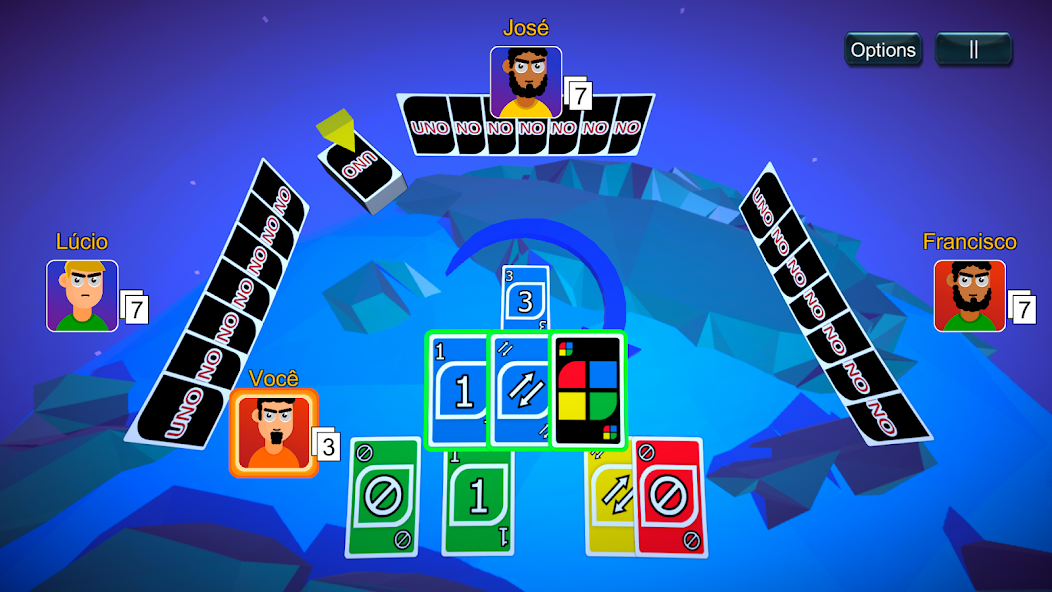
\includegraphics[width=0.5\textwidth]{img/image.png} % Adjust the width as needed
    \caption{Intro Scene}
    \label{fig:intro-scene}
\end{figure}

\textbf{Description}: These are the interfaces we are trying to achieve. In this interface, each player has a visual on all of their card deck, which they click on a preferred card, and it will be added to the center. And a player can only see their card deck, and the others are folded.

\textcolor{white}{This text is invisible but takes up space.} \\
Another related work that gives us idea on working with the winner scene is Kahoot outro \cite{b3}, which introduces the game winner.
\begin{figure}[h!]
    \centering
    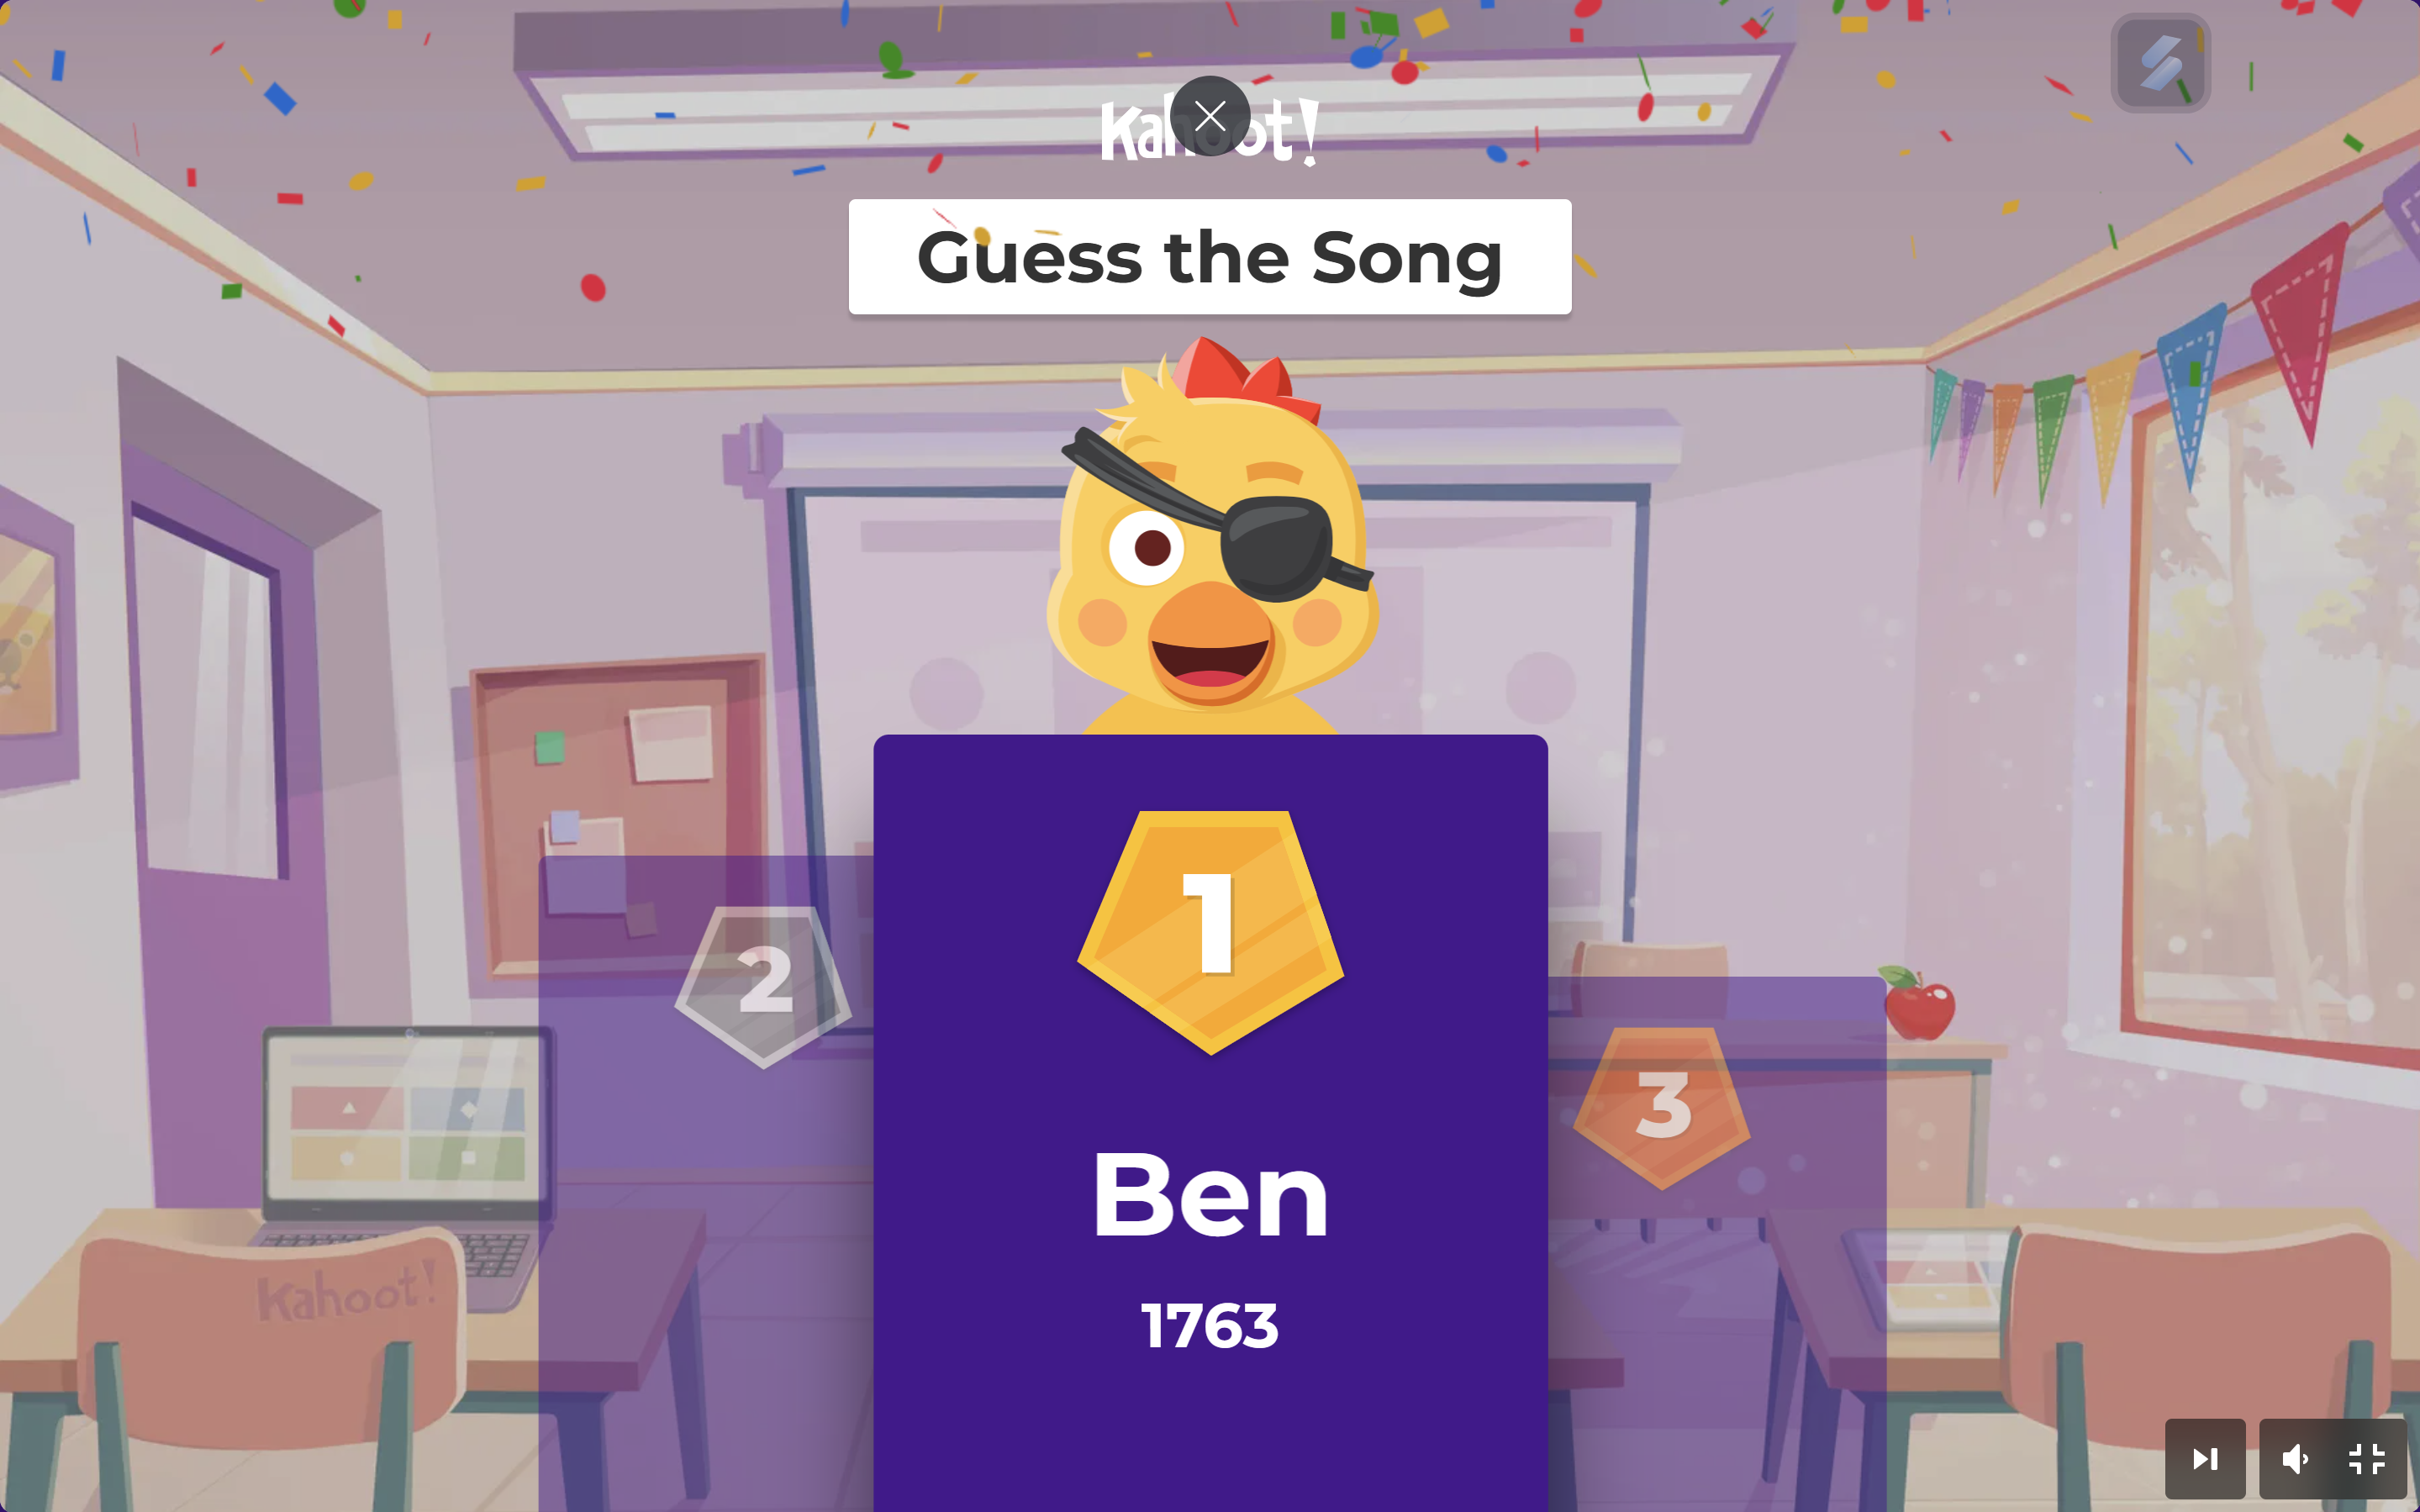
\includegraphics[width=0.5\textwidth]{img/Screenshot 2025-01-14 134455.png} % Adjust the width as needed
    \caption{Winner Scene}
    \label{fig:winner-scene}
\end{figure}

\textbf{Description}: This is the outro that gives us ideas to introduce the winner. It is same as a podium, that introduces the 3rd place first, and then moves to the right, 2nd place later, then moves to the left and finally the 1st player, and move to the center.

\section{Team Work}
In this section, we will discuss about the process of team work and the work structure of our project.


\subsection{Who does what?}
This team consists of 3 members: Dat, Nguyen, and Khoa. Below is the distribution of work process.
\begin{itemize}
    \item Dat: Responsible for distribution of work for team members. Also responsible for researching and working with GUI(Javafx \& Scene Builder). Moreover Dat is responsible for communications between team members and updates to the project workflow.
    
    \item Nguyen: Responsible for determining the classes, the workflow and logic code for score calculation. Working with Dat, Nguyen is responsible for the drawing and explanation of the diagrams.

    \item Khoa: Responsible for applying Dat's code to create a new version of GUI for single player.
\end{itemize}

Each week, the team will have an online meeting on Google Meet to update the work process to Dat. 

\subsection{Work Structure}   
Work Timeline: Here are our main timeline of the project:
\begin{enumerate}
    \item 05/12/2024: Choose board game topic for the project.
    \item 08/12/2024 - 10/12/2024: Understand rules, define classes, outline, skeleton of the project.
    \item 11/12/2024 - 12/12/2024: Set up the extension, build up the project.
    \item 12/12/2024 - 17/12/2024: Work with code, finish the logic code and run the game in Command Line.
    \item 18/12/2024 - 30/12/2024: Assign Khoa to implement the GUI of the board game.
    \item 01/01/2025 - 03/01/2025: Khoa's realization of errors and rework again with GUI.
    \item 04/01/2025 - 12/01/2025: Dat's research, implementation of another version of GUI of the game. 
    \item 13/01/2025 - 17/01/2025: Dat, Khoa, Nguyen finish the documentation of report.
    \item 18/01/2025 - 22/01/2025: Implement the gameplay to check for error of logic and GUI. End the project.
\end{enumerate}


    
\subsection{Ideas}
The initial idea when we brainstorm is to create a board and make cards to move in the center area like poker and some card games. There are other ideas on using numbers from 1 to 5 to choose the preferred card each round.  One member is responsible for outlining the game component while the 2 others determine the layout of the game and how to interact with the game.

Then it comes to the set up idea to stick with the second way to work with Command Line to test and implement the logic first. Then 2 members will independently apply the logic and create 2 versions of GUI for gameplay, which is single player and multiplayer

In the maintenance part, the member that is responsible for logic code is responsible for testing the game and reporting back to the member implementing GUI if there are errors in relation to the game components or logics of the game.  

\section{Proposed Approaches}

\textbf{Algorithms in Pseudocode:}

\begin{enumerate}
    \item Initialize class variables:
    \begin{itemize}
        \item List of farms
        \item List of players
        \item List of cards (deck)
        \item List of cards (discard pile)
        \item Die object
        \item List of corn cubes
        \item Corn counts (green, blue, yellow)
    \end{itemize}

    \item Constructor Game():
    \begin{itemize}
        \item Initialize cubes list with green, blue, and yellow corn types
    \end{itemize}

    \item Method getCubes():
    \begin{itemize}
        \item Return cubes list
    \end{itemize}

    \item Constructor Game(playerCount):
    \begin{itemize}
        \item Call initializeFarms()
        \item Call initializeDeck()
        \item Call initializePlayers(playerCount)
        \item Call addInitialCorn()
    \end{itemize}

    \item Method getDeck():
    \begin{itemize}
        \item Return deck list
    \end{itemize}

    \item Method initializeFarms():
    \begin{itemize}
        \item Add farms with predefined colors to farms list
    \end{itemize}

    \item Method initializeDeck():
    \begin{itemize}
        \item Add cards of different types and colors to deck
        \item Shuffle the deck
    \end{itemize}

    \item Method initializePlayers(playerCount):
    \begin{itemize}
        \item Create players and deal 5 cards to each from the deck
    \end{itemize}

    \item Method addInitialCorn():
    \begin{itemize}
        \item Add initial corn cubes to farms randomly
    \end{itemize}

    \item Method startGame():
    \begin{itemize}
        \item Loop until game ends (no more corns to distribute):
        \begin{itemize}
            \item Print farms
            \item Players pick cards
            \item Resolve cards
            \item Display player score piles
            \item Display corn counts
            \item Display deck and discard pile counts
            \item Check if game should end
            \item Deal new cards to players
        \end{itemize}
    \end{itemize}

    \item Method printFarms():
    \begin{itemize}
        \item Print each farm
    \end{itemize}

    \item Method pickCardForPlayer(player, scanner):
    \begin{itemize}
        \item Allow player to pick a card from their hand
        \item Return chosen card
    \end{itemize}

    \item Method resolveCards(chosenCards):
    \begin{itemize}
        \item Group cards by color
        \item Resolve each farm based on grouped cards
        \item Display player scores after resolving actions
    \end{itemize}

    \item Method resolveFarm(cards, farm):
    \begin{itemize}
        \item Separate cards into birds, foxes, and fleeing birds
        \item Resolve fleeing birds if no foxes
        \item Resolve foxes and birds if both present
        \item Resolve birds if only birds present
        \item Resolve foxes if only foxes present
    \end{itemize}

    \item Method resolveBirds(birds, farm):
    \begin{itemize}
        \item Sort birds by player name
        \item If one bird, it eats all corn
        \item If multiple birds, they fight for corn
        \item Add played bird cards to discard pile
    \end{itemize}

    \item Method resolveFoxesAndBirds(foxes, birds, fleeingBirds, farm):
    \begin{itemize}
        \item Sort foxes by player name
        \item Determine winning fox
        \item Winning fox eats all birds
        \item Add played fox and bird cards to discard pile (eaten birds will not be added, the fox player keeps them)
    \end{itemize}

    \item Method resolveFoxes(foxes):
    \begin{itemize}
        \item Sort foxes by player name
        \item Add played fox cards to discard pile
    \end{itemize}

    \item Method resolveFleeingBird(fleeingBirds, farm, otherBirdsAndFoxes):
    \begin{itemize}
        \item If fleeing bird is alone, it eats all corn
        \item If not alone, it takes one green corn if available
    \end{itemize}

    \item Method resolveFleeingBirdDiscard(fleeingBirds, farm, otherBirdsAndFoxes):
    \begin{itemize}
        \item If fleeing bird is alone, it eats all corn
        \item If not alone, it takes one green corn if available
        \item Add played fleeing bird cards to discard pile
    \end{itemize}

    \item Method addCornToFarms():
    \begin{itemize}
        \item Add corn cubes to farms randomly based on available corn types
    \end{itemize}

    \item Method dealNewCards():
    \begin{itemize}
        \item Shuffle discard pile into deck if needed
        \item Deal new cards to players
    \end{itemize}

    \item Method declareWinner():
    \begin{itemize}
        \item Determine player with highest score and declare winner
    \end{itemize}

    \item Main method:
    \begin{itemize}
        \item Print welcome message
        \item Get number of players from user
        \item Create Game object with player count
        \item Start the game
        \item Close scanner
    \end{itemize}
\end{enumerate}

\vspace{0.2cm}

\textbf{Summary:}

This pseudocode outlines how players interact through farms, cards, and corn resources. The game starts by initializing key components, including farms, players, a shuffled deck, a discard pile, and corn cubes of different types. Players are dealt cards and take turns picking and resolving them, with gameplay focusing on how birds, foxes, and fleeing birds interact at farms to compete for corn. Birds eat corn or fight each other, foxes prey on birds, and fleeing birds act selectively based on the presence of other cards. The game progresses in a loop, where farms are updated, resources are redistributed, and new cards are dealt to players, with the game state displayed at each step. The loop ends when there are not enough corns to distribute, at which point the player with the highest score is declared the winner.

\section{Implementation Details}

In this section, we will introduce the application structure, which will presents the game logic layer(Model), User Interface layer(View), Controller layer, and the resources of the project. Moreover, we will explain carefully the GUI details and give instructions about the UML diagrams and libraries used to run the game. 
\subsection{Application Structure}
\subsubsection{Game Logic Layer}
\paragraph{Role}
First and foremost is the Game Logic layer(Model), which contains the core game logic, which contains classes for game rules, objects, and player state management.

\paragraph{Responsibility}
\begin{itemize}
    \item Implement the game rules, logics and mechanics
    \item Manage and update the cards, cubes states and players' scores.
\end{itemize}

\paragraph{Model components}
\begin{itemize}
    \item Card.java: This contains the class and the components of a card. It contains the type, color and value of cards, and the constructors, getter, setter function to call the card. A card can be valued from 3 to 6 for Bird, 4 to 6 for Fox, and -2 for Fleeing Bird. A card has 6 colors: Including Yellow, Green, Red, Blue, Purple, and Black.
    \item CornCube.java: This contains the class and the types of the corn, functions to value the points based on the color, which is 1, 2, or 3. 
    \item Die.java: This contains a parameter to random a score from 1 to 6, which corresponds the values of a die.
    \item Farm.java: This contains a parameter color and a list of corns, which is defined in CornCube.java. The farm has also 6 colors, as same as Card. It also has methods to add corns and clear corns, which are functions used in game.
    \item Game.java: This contains methods to initialize the game, declare number of cards for player, add and remove cards, add and remove corns, and calculate the players' scores after each round. Gameplay on Command Line can be played here.
    \item Player.java: This contains parameter of name of players, which are set to player 1, 2, and 3. It has methods to add new card from Card Deck, add to player's current score.
\end{itemize}

\subsubsection{User Interface Layer(View)}
\paragraph{Role}
Next is the User Interface Layer, which defines the Graphical User Interface (GUI) of the application. This layer is built using Scene Builder and added to the application under FXML files for a clean separation of UI design and application logic.

\paragraph{Responsibilities}
\begin{itemize}
    \item Display the game boards, cards images, and other UI components, including the buttons to start and end game, or to function the game.
    \item Handle User Interaction as real-life board game.
\end{itemize}

\paragraph{Interface Components}
\begin{itemize}
    \item begin.fxml: Begin menu view, which is the intro of the game.
    \item rules.fxml: Rule view, where players can understand rules of playing and score calculations.
    \item game.fxml: The main board game view, where players can interact with the game.
    \item winner.fxml: The board view to finalize and introduce the winner of the game.
    \item styles.css: Stylesheets for customization of User Interface elements.
    \item WinnerAnimation.java: Contains the animations to celebrate the winner in winner board view.
\end{itemize}

\subsubsection{Controller Layer}
\paragraph{Role}
The Controller Layer acts as a bridge between the Game Logic layer (Model) and the Interface layer (View). It contains Java controller classes linked to FXML files, using FXML:Controller atrributes.

\paragraph{Responsibilities}
\begin{itemize}
    \item Handle user interactions (Button clicks, Cards moving, Corns adding, etc.).
    \item Update the view based on the game state and logic.
\end{itemize}

\paragraph{Controller Components}
\begin{itemize}
    \item BeginController.java: Manage begin scene and enable users to start the game, change to rules view or exit the game. Moreover, this controller create transition from begin scene to game scene smoothly.
    \item MainController.java: Manage the game scene and enable user interactions with games, calculate score for players and handle the discarded card. This controller make transition  from game scene to winner scene when the condition is satisfied.
    \item WinnerController.java: Manage the winner scene and apply the animations to the winner scene. It also handles the actions to play again or exit the game.
\end{itemize}

\subsection{Resources}
\paragraph{Roles}
The resources contain static assets such as images of card, farms and gifs for animation. 

\paragraph{Components}
\begin{itemize}
    \item images/: Folder contains farms' images for game decorations.
    \item begin/: Folder contains image for the begin scene.
    \item cards/: Folder contains cards' images for game decorations.
    \item gif/: folder contains gifs and image used in the rules scene and game decorations.
    \item logo/: Folder contains the logo for the game bar decoration. 
\end{itemize}

\subsection{GUI Details}
In this section, we will introduce and explain how the scenes are created and how to handle the interactions in each scene.

First, we take the images of the games, which have the images of cards, farms to create the interface for the main game. As discussed in \cite{b5} we take screenshots of each card image and farm image and create an \textbf{ImageView} for each area, which will be seen in the game scene.
\begin{figure}[h!]
    \centering
    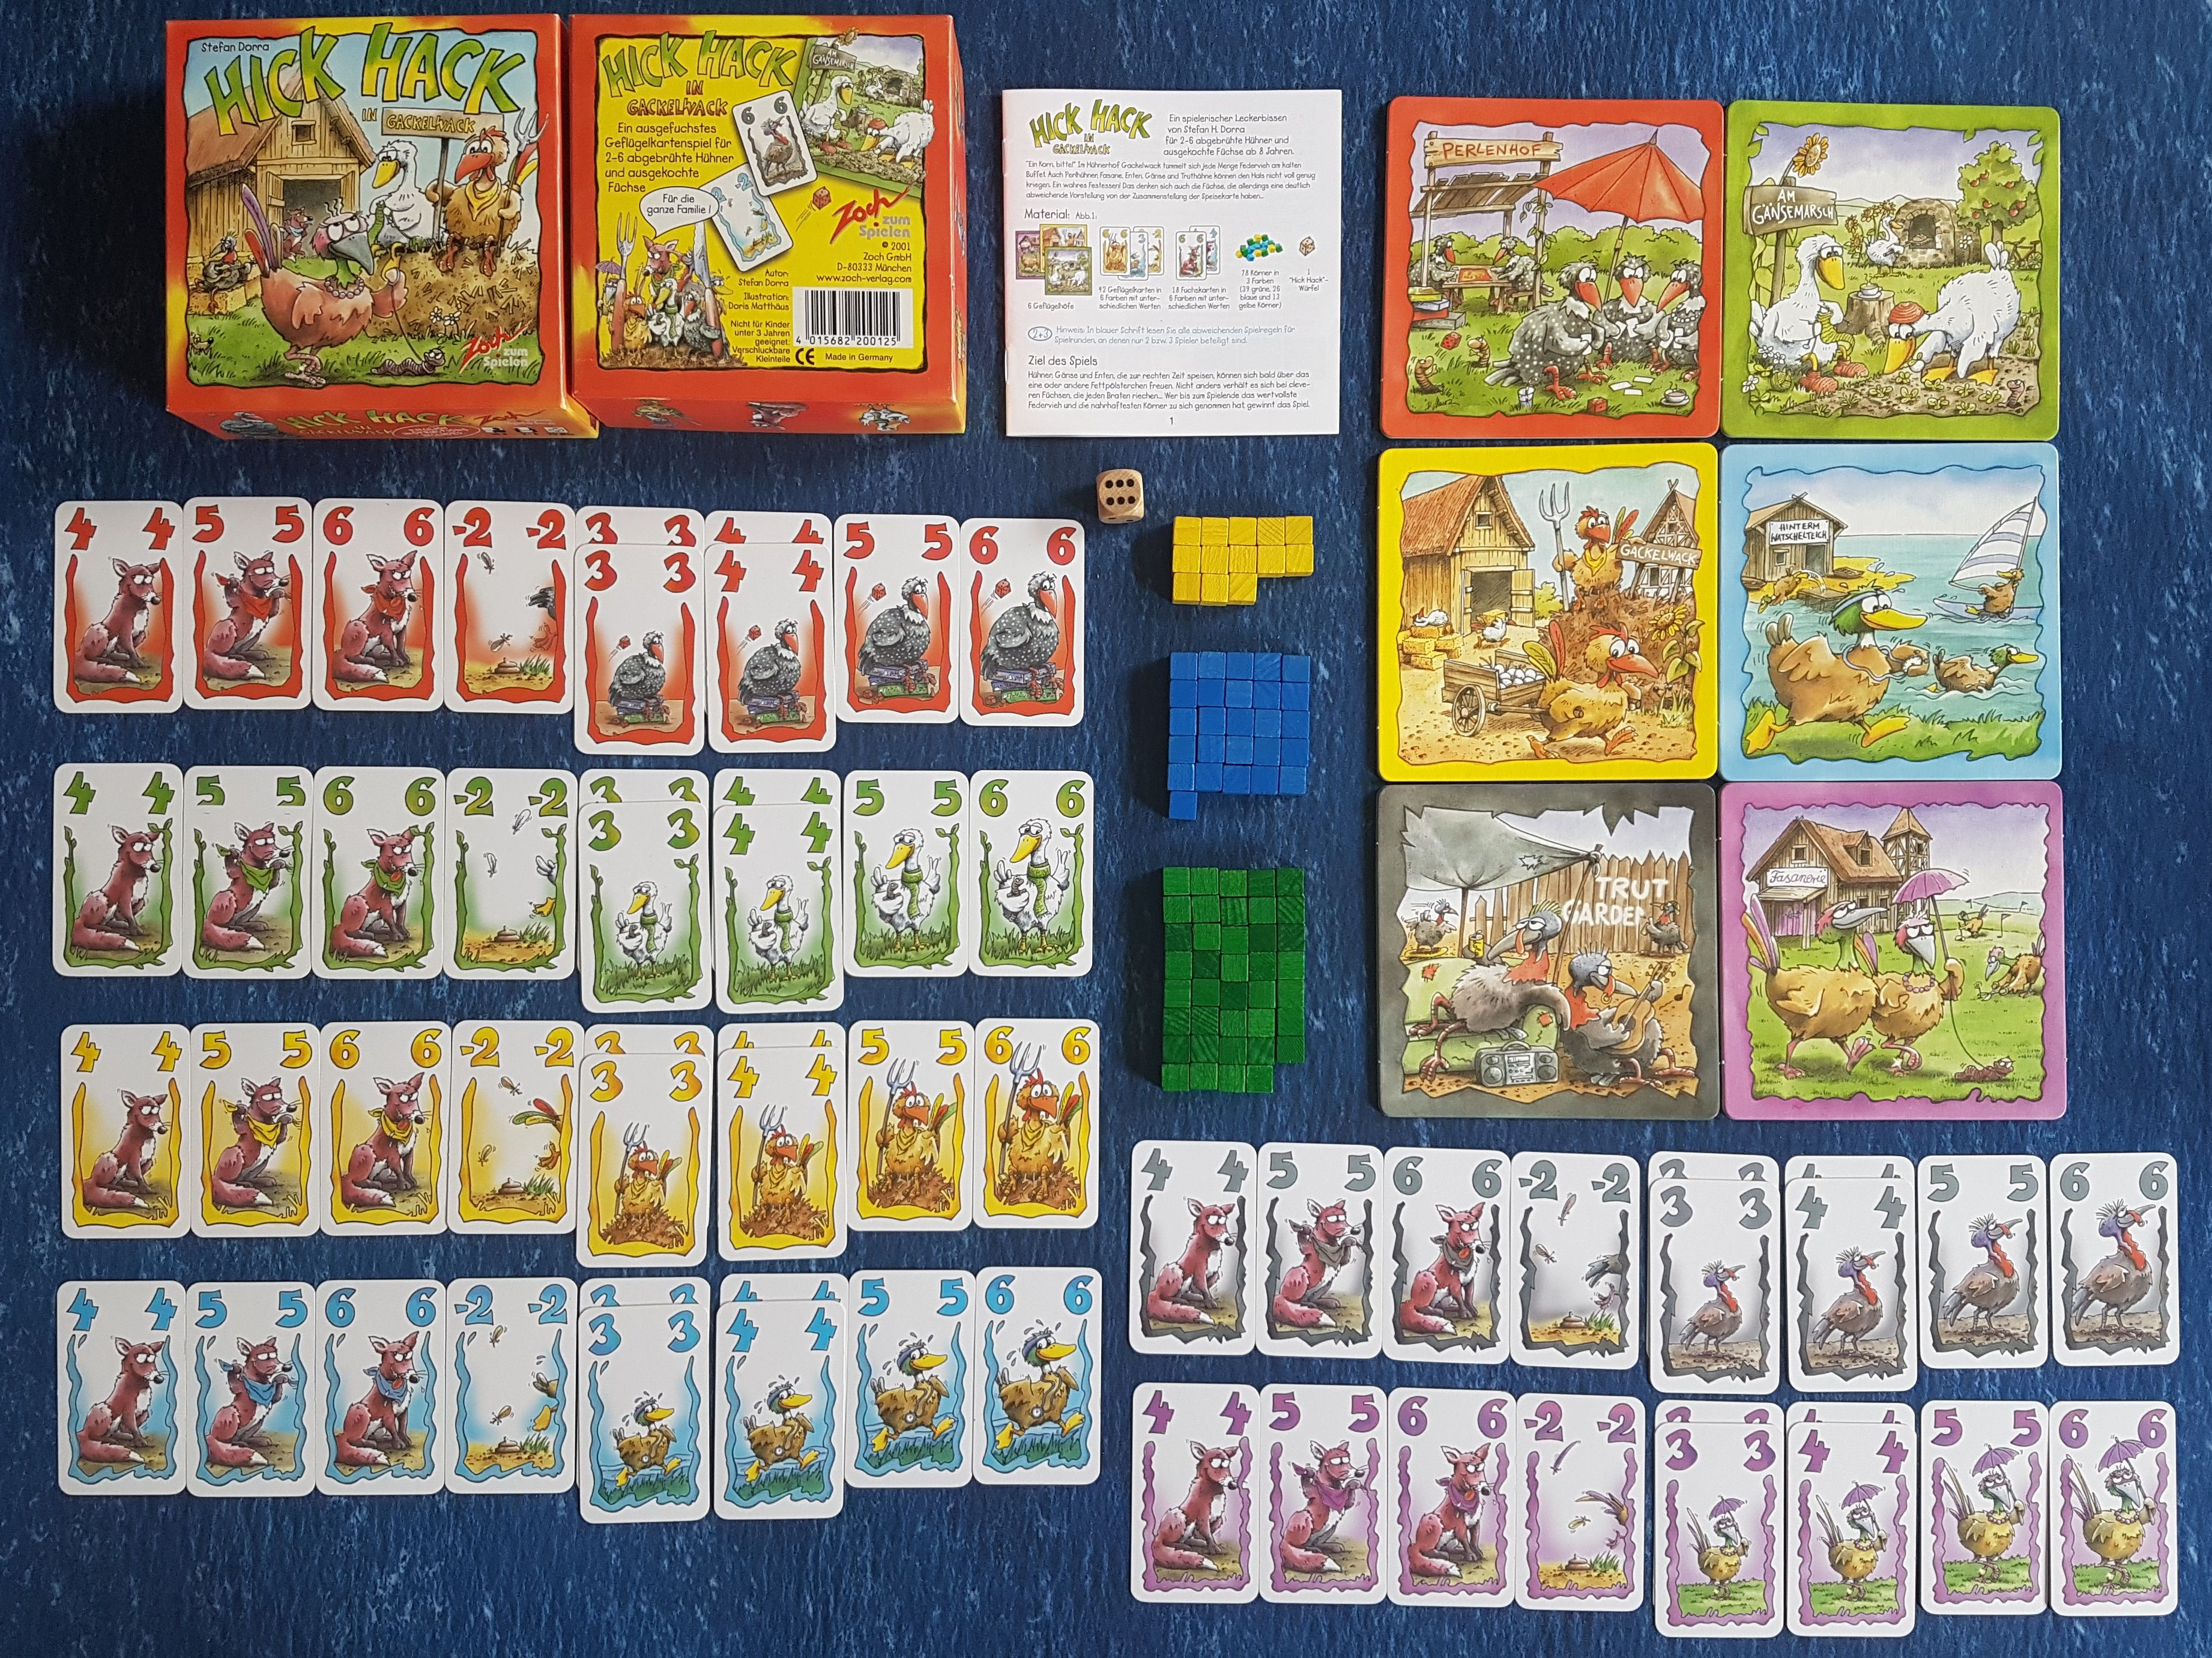
\includegraphics[width=0.4\textwidth]{img/465654734_8820796054708413_4663815448351147464_n.jpg} % Adjust the width as needed
    \caption{HickHack Game Image}
    \label{fig:intro-scene}
\end{figure}


\textbf{Intro Scene:}
This scene is the introduction of our game.
\begin{figure}[h!]
    \centering
    \includegraphics[width=0.4\textwidth]{img/Screenshot 2025-01-17 150200.png} % Adjust the width as needed
    \caption{Intro Scene}
    \label{fig:intro-scene}
\end{figure}

The \textbf{background image} in the code is the background image in the scene, which is used to decorate the intro. The 2 labels \textbf{title Label} and \textbf{welcome Label} are the lines appearing in the intro, which there are 3 buttons, including \textbf{Start Game}, \textbf{Show Rules}, and \textbf{Exit} are buttons that make transitions to the corresponding scenes or exit the game.

\vspace{2cm}

\begin{lstlisting}[language = Python, caption = Start Game Button, basicstyle=\footnotesize, frame=single, framesep=1pt, framerule=0.5pt, xleftmargin=8pt, xrightmargin=8pt]
    @FXML
    public void onOkButtonPressed(ActionEvent event) {
        int playerCount = 3; // Fixed number of players
        game = new Game(playerCount); // Initialize the game with the number of players
        if (mainApp != null) {
            mainApp.showGamePage(game); // Pass the game instance to the game page
        } else {
            System.err.println("mainApp is null, cannot proceed.");
        }
    }
\end{lstlisting}

\vspace{0.5cm}

\begin{lstlisting}[language = Java, caption= Show Rules Button, frame=single, basicstyle=\footnotesize, framesep=1pt, framerule=0.5pt, xleftmargin=8pt, xrightmargin=8pt]
    @FXML
    private void handleShowRulesAction(ActionEvent event) {
        if (mainApp != null) {
            mainApp.showRulesPage();
        } else {
            System.err.println("mainApp is null, cannot proceed.");
        }
    }
    
\end{lstlisting}

\vspace{0.5cm}

\begin{lstlisting}[language = Java, caption = Single Player Button , basicstyle=\footnotesize, frame=single, framesep=1pt, framerule=0.5pt, xleftmargin=8pt, xrightmargin=8pt ]
    @FXML
     public void handleSinglePlayerButtonAction(ActionEvent event) {
         int playerCount = 3;
         game = new Game(playerCount);
         if (mainApp != null) {
                mainApp.showSinglePage(game);
            } else {
                System.err.println("mainApp is null, cannot proceed.");
         }
     }
\end{lstlisting}

\vspace{0.5cm}

\begin{lstlisting}[language = Java, caption = Exit Button, basicstyle=\footnotesize, frame=single, framesep=1pt, framerule=0.5pt, xleftmargin=8pt, xrightmargin=8pt ]
    @FXML
    public void handleExitAction(ActionEvent event) {
        Stage stage = (Stage) ((Button) event.getSource()).getScene().getWindow();
        stage.close();
    }
\end{lstlisting}

\textcolor{white}{This text is invisible but takes up space.} \\

\newpage
    
\textbf{Game Rules Scene:}

This is the Rules Scene if players click the \textbf{Show Rules} Button
\begin{figure}[h!]
    \centering
    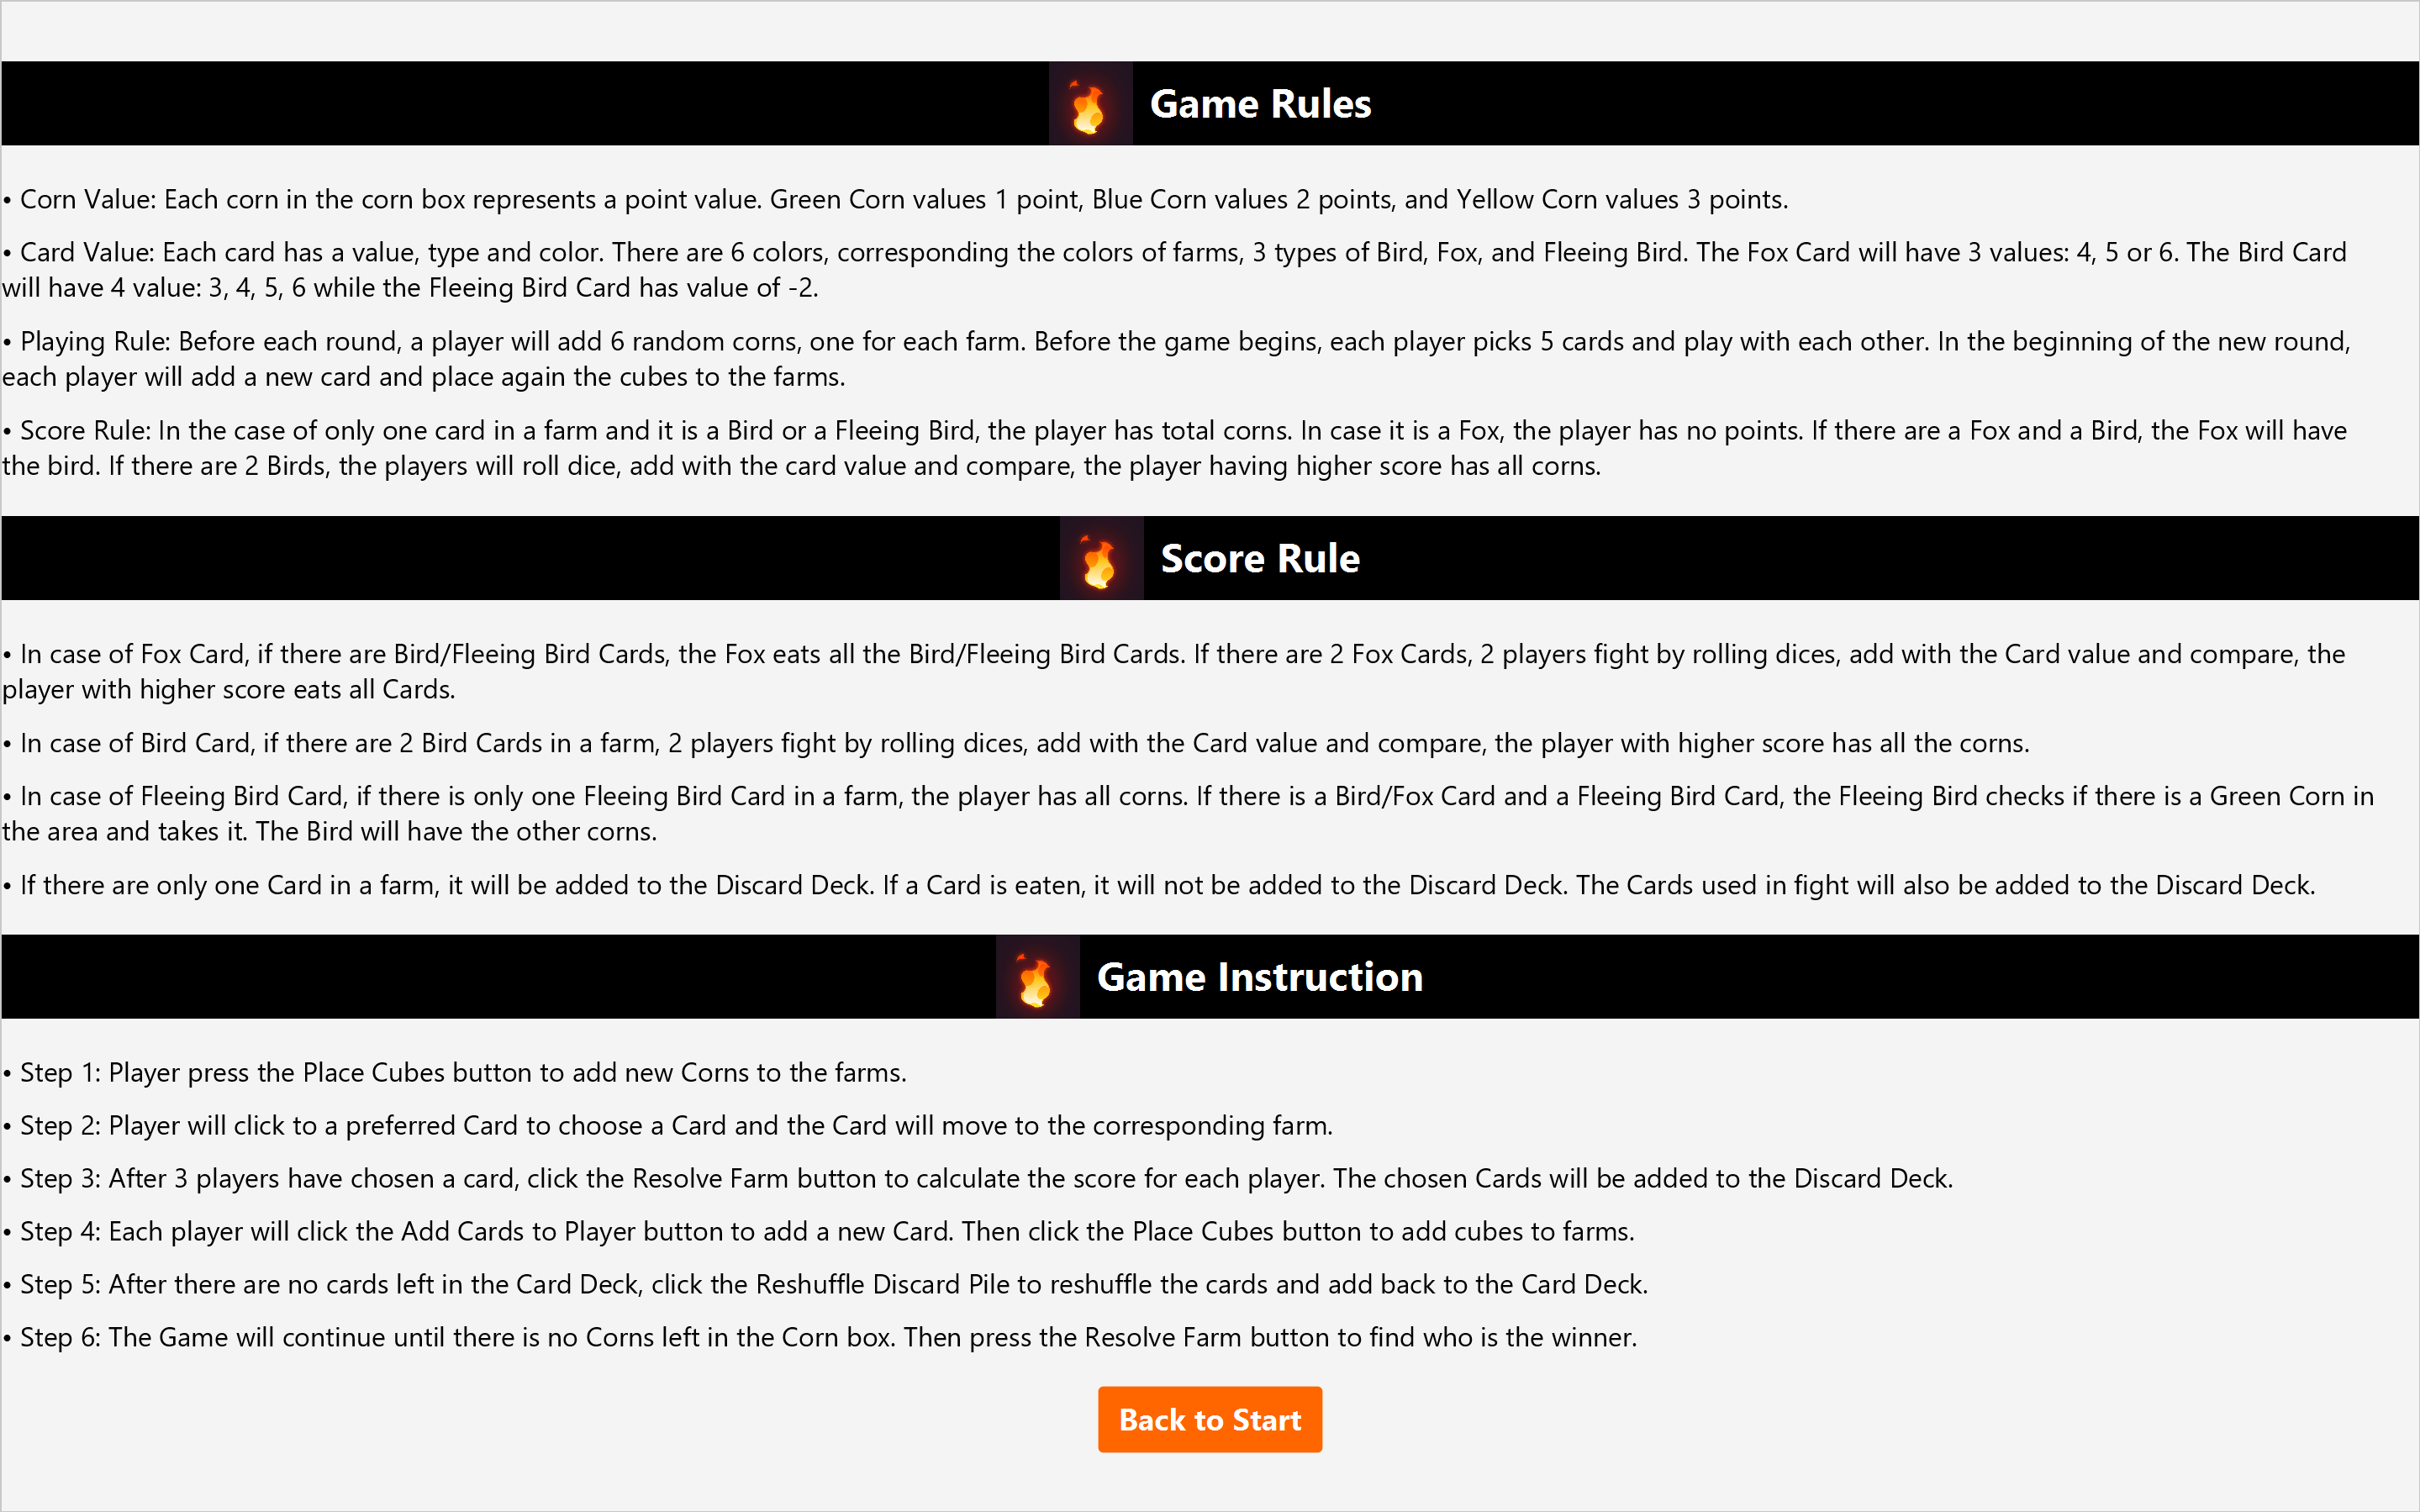
\includegraphics[width=0.5\textwidth]{img/Screenshot 2025-01-14 111830.png} % Adjust the width as needed
    \caption{Rules Scene}
    \label{fig:rule-scene}
\end{figure}

In this scene, there are full description of the rules:
\begin{itemize}
    \item \textbf{Game Rules}: show how to play the game.
    \item \textbf{Score Rules}: show how to calculate players' score.
    \item \textbf{Game Instructions}: show how to play the games, click the button and how to choose cards.
\end{itemize}
If players click the \textbf{Back to Start} button, the game will return back to intro scene.

\begin{lstlisting}[language = FXML, caption = Back to Start Button, basicstyle=\scriptsize, frame=single, framesep=1pt, framerule=0.5pt, xleftmargin=8pt, xrightmargin=8pt]
    @FXML
    private void handleBackToStartAction(ActionEvent event) {
        try {
            // Load the begin.fxml file
            FXMLLoader loader = new FXMLLoader(getClass().getResource("/hellofx/resources/begin.fxml"));
            Parent root = loader.load();

            // Get the controller and set the mainApp reference
            BeginController beginController = loader.getController();
            beginController.setMainApp(mainApp);

            // Get the current stage
            Stage stage = (Stage) ((Button) event.getSource()).getScene().getWindow();

            // Set the new scene
            stage.setScene(new Scene(root));
            stage.setFullScreen(true); // Set the stage to full screens
            stage.show();
        } catch (Exception e) {
            e.printStackTrace();
        }
    }
    
\end{lstlisting}

\vspace{1.5cm}
\textbf{Single Player Scene: }
This is the game scene, when players click the \textbf{Single Player} Button.

\begin{figure}[h!]
    \centering
    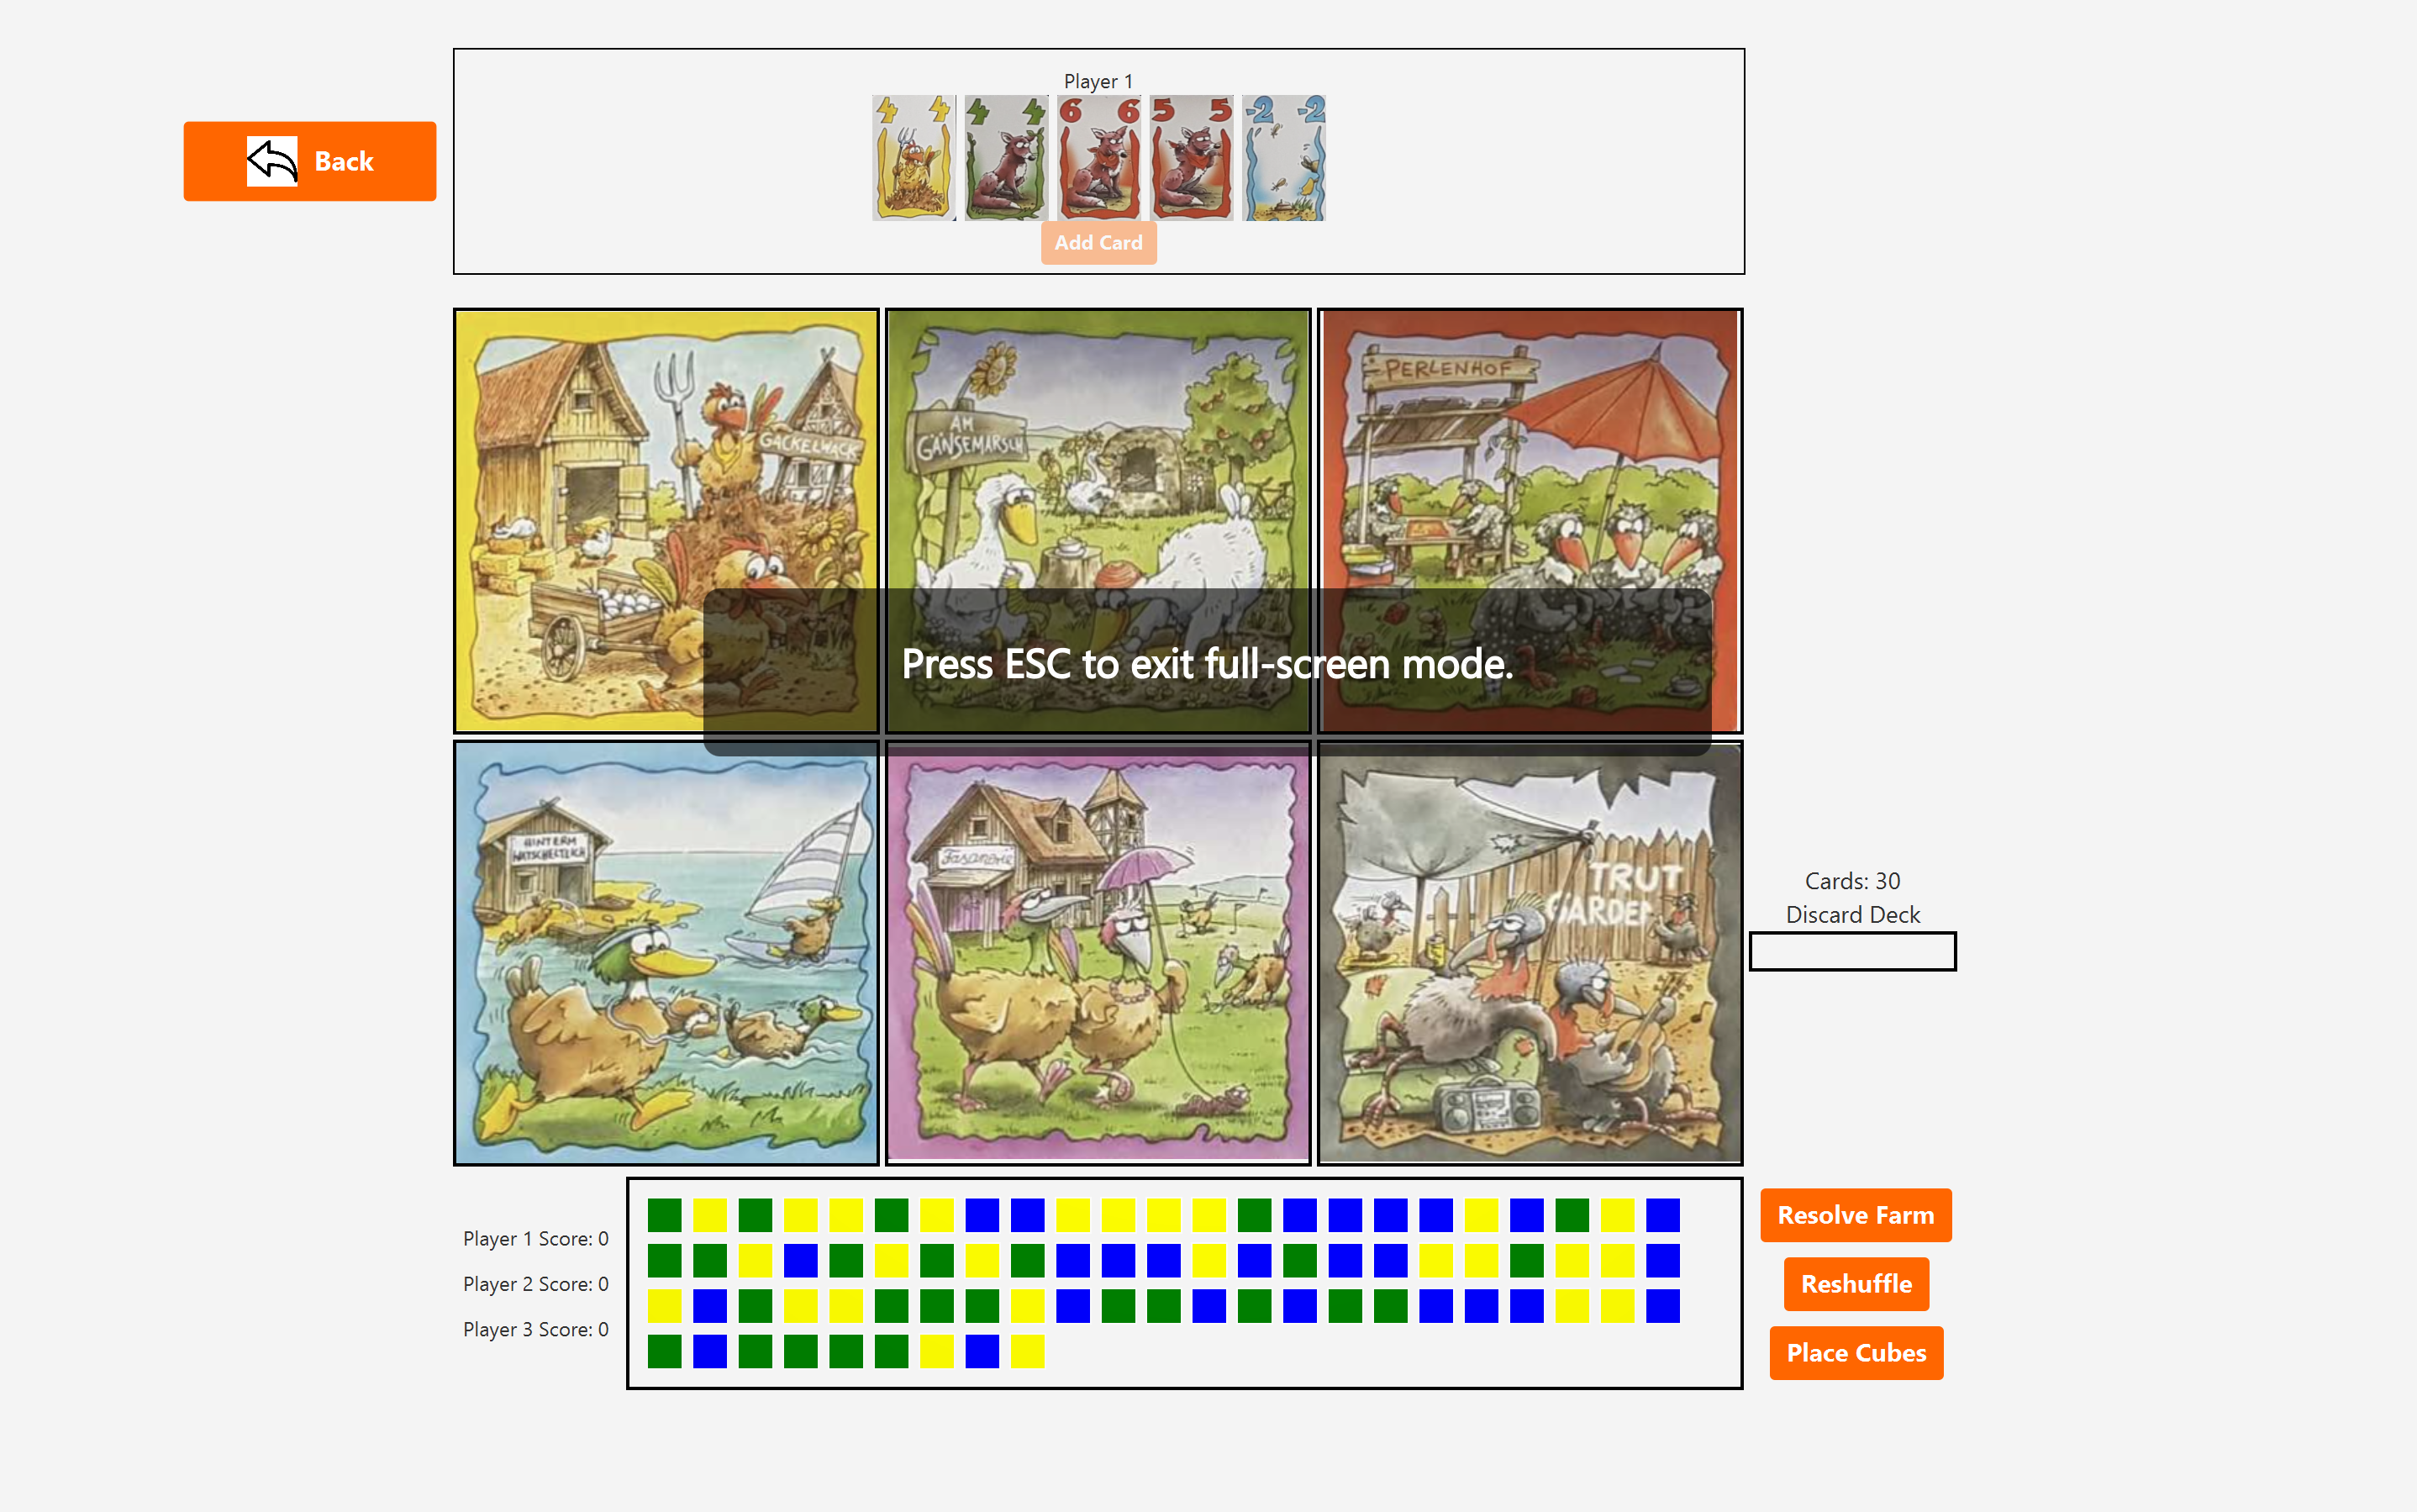
\includegraphics[width=0.5\textwidth]{img/Screenshot 2025-01-17 150553.png} % Adjust the width as needed
    \caption{Single Player Scene}
    \label{fig:game-scene}
\end{figure}

\vspace{1cm}

\textbf{Multiplayer Game Scene: }
This is the game scene, when players click the \textbf{Start Game} Button.
\begin{figure}[h!]
    \centering
    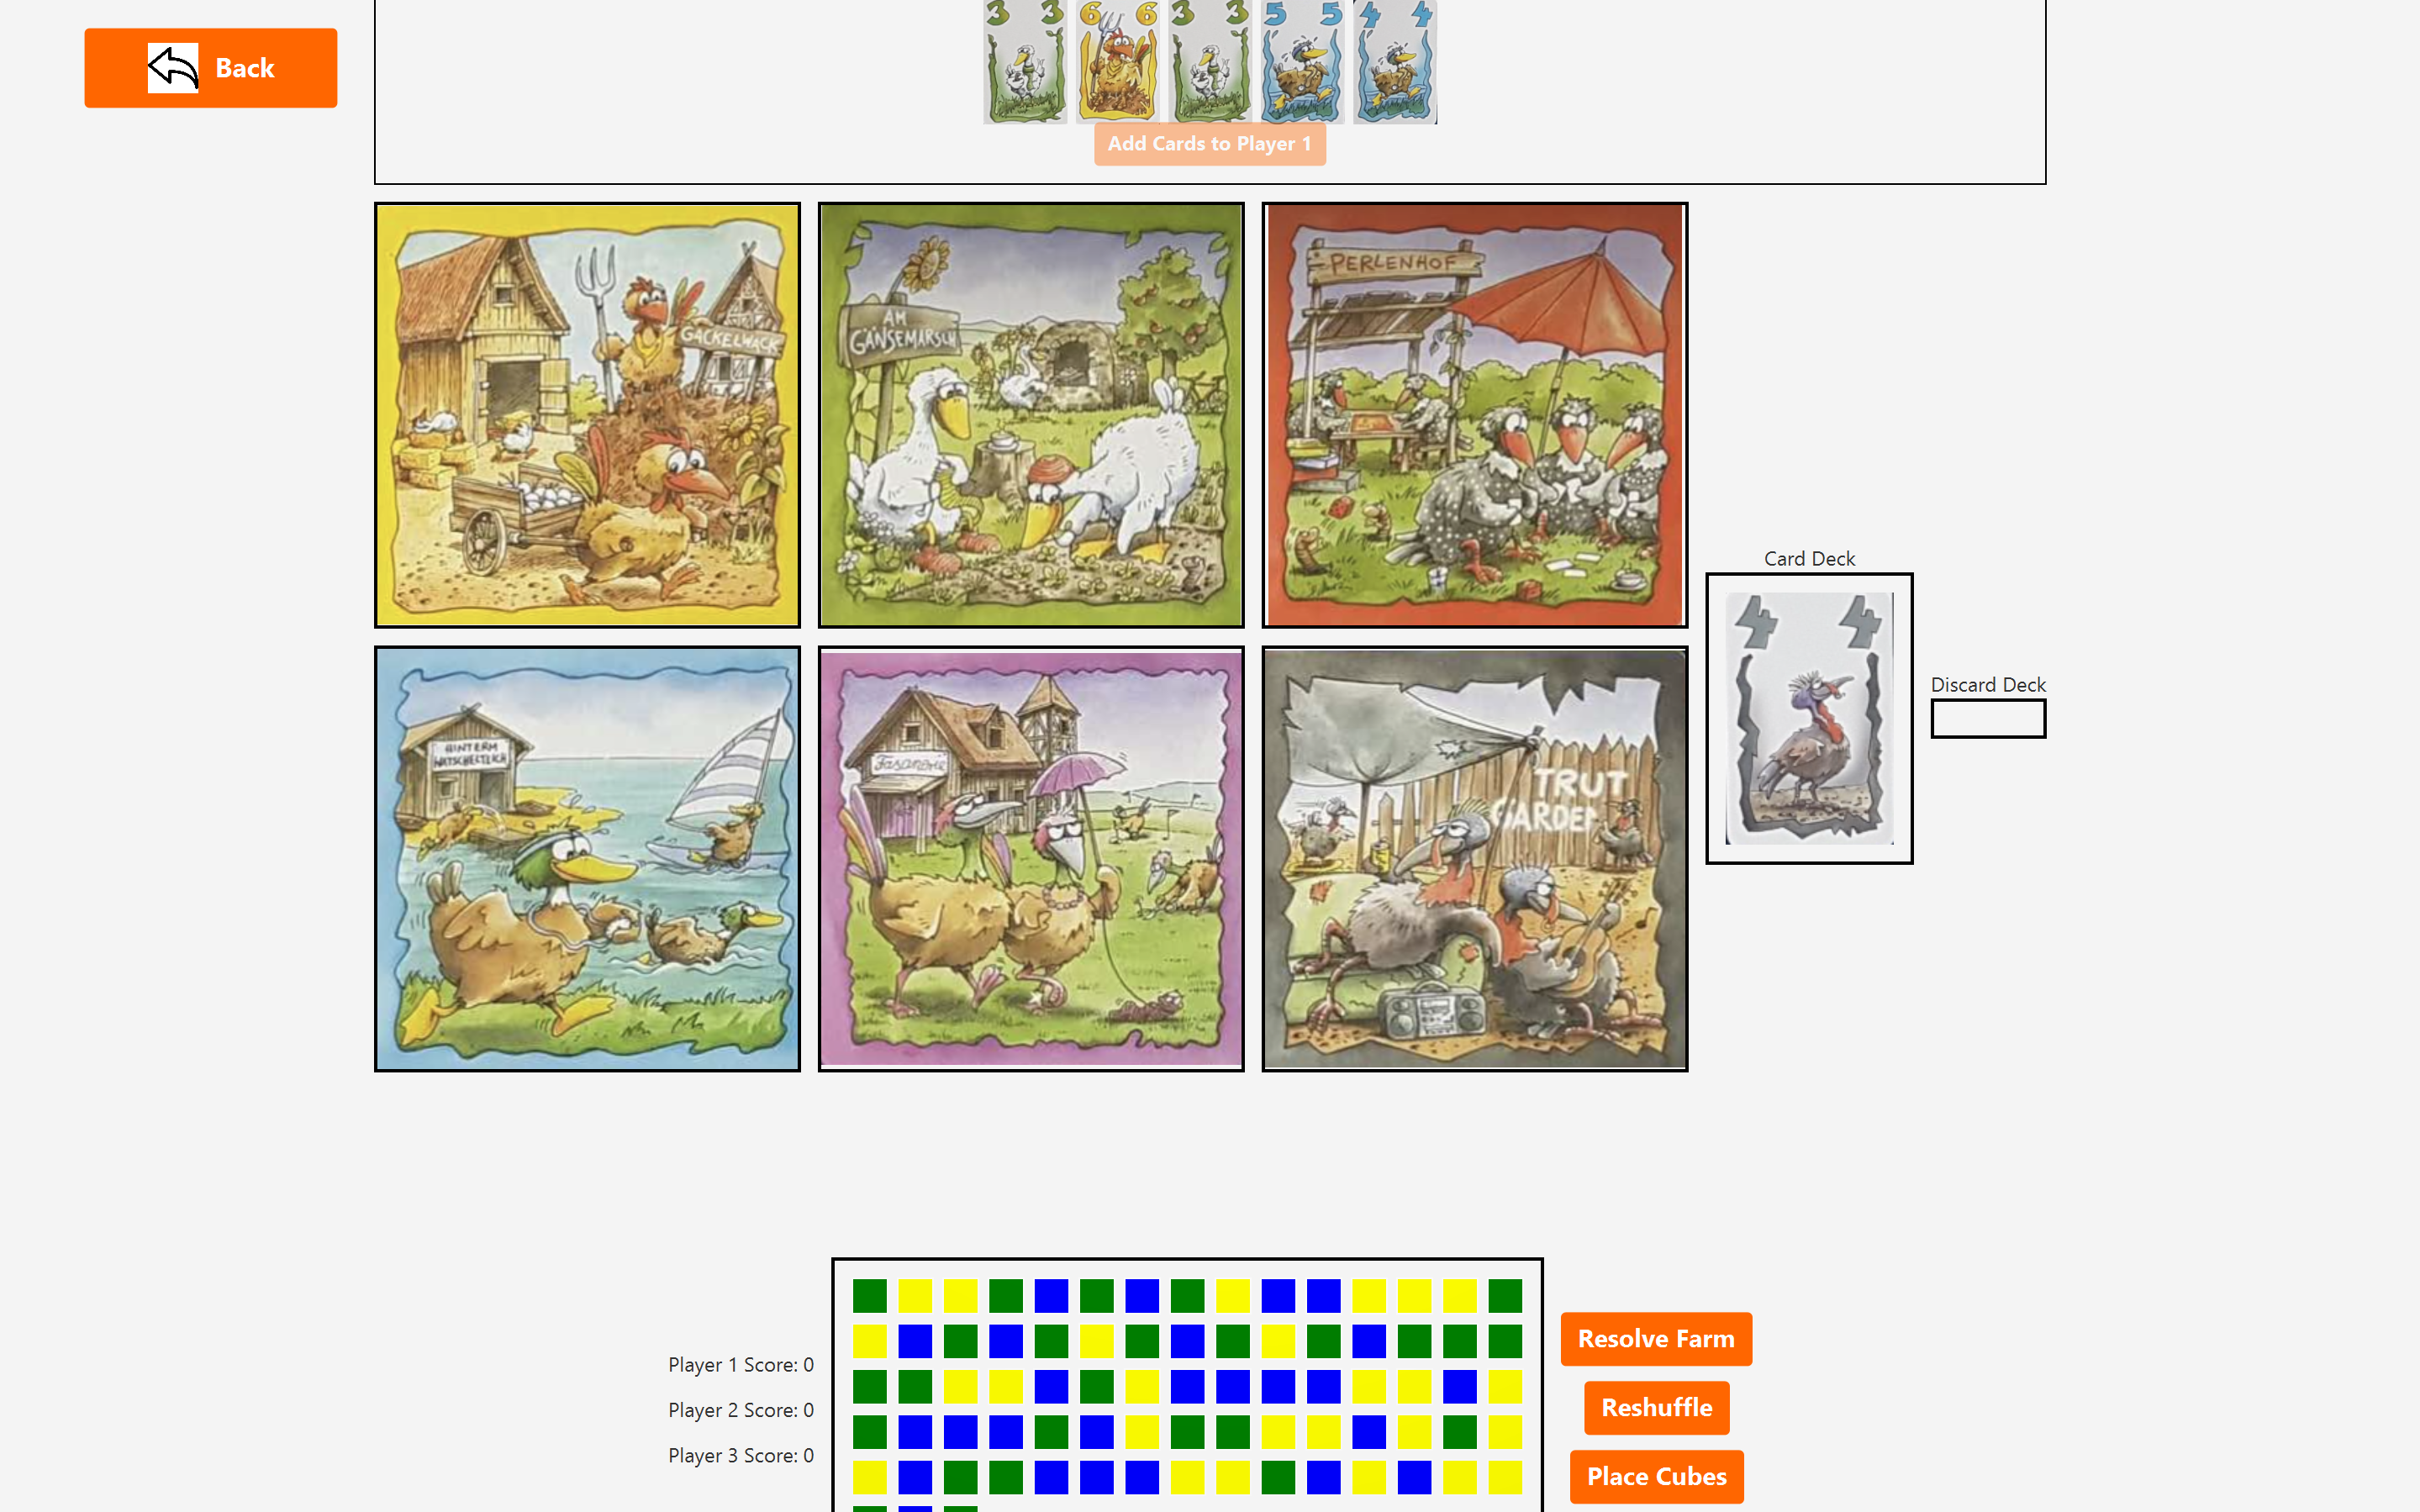
\includegraphics[width=0.5\textwidth]{img/Screenshot 2025-01-14 113548.png} % Adjust the width as needed
    \caption{Game Scene player 1 turn}
    \label{fig:game-scene}
\end{figure}

\begin{figure}[h!]
    \centering
    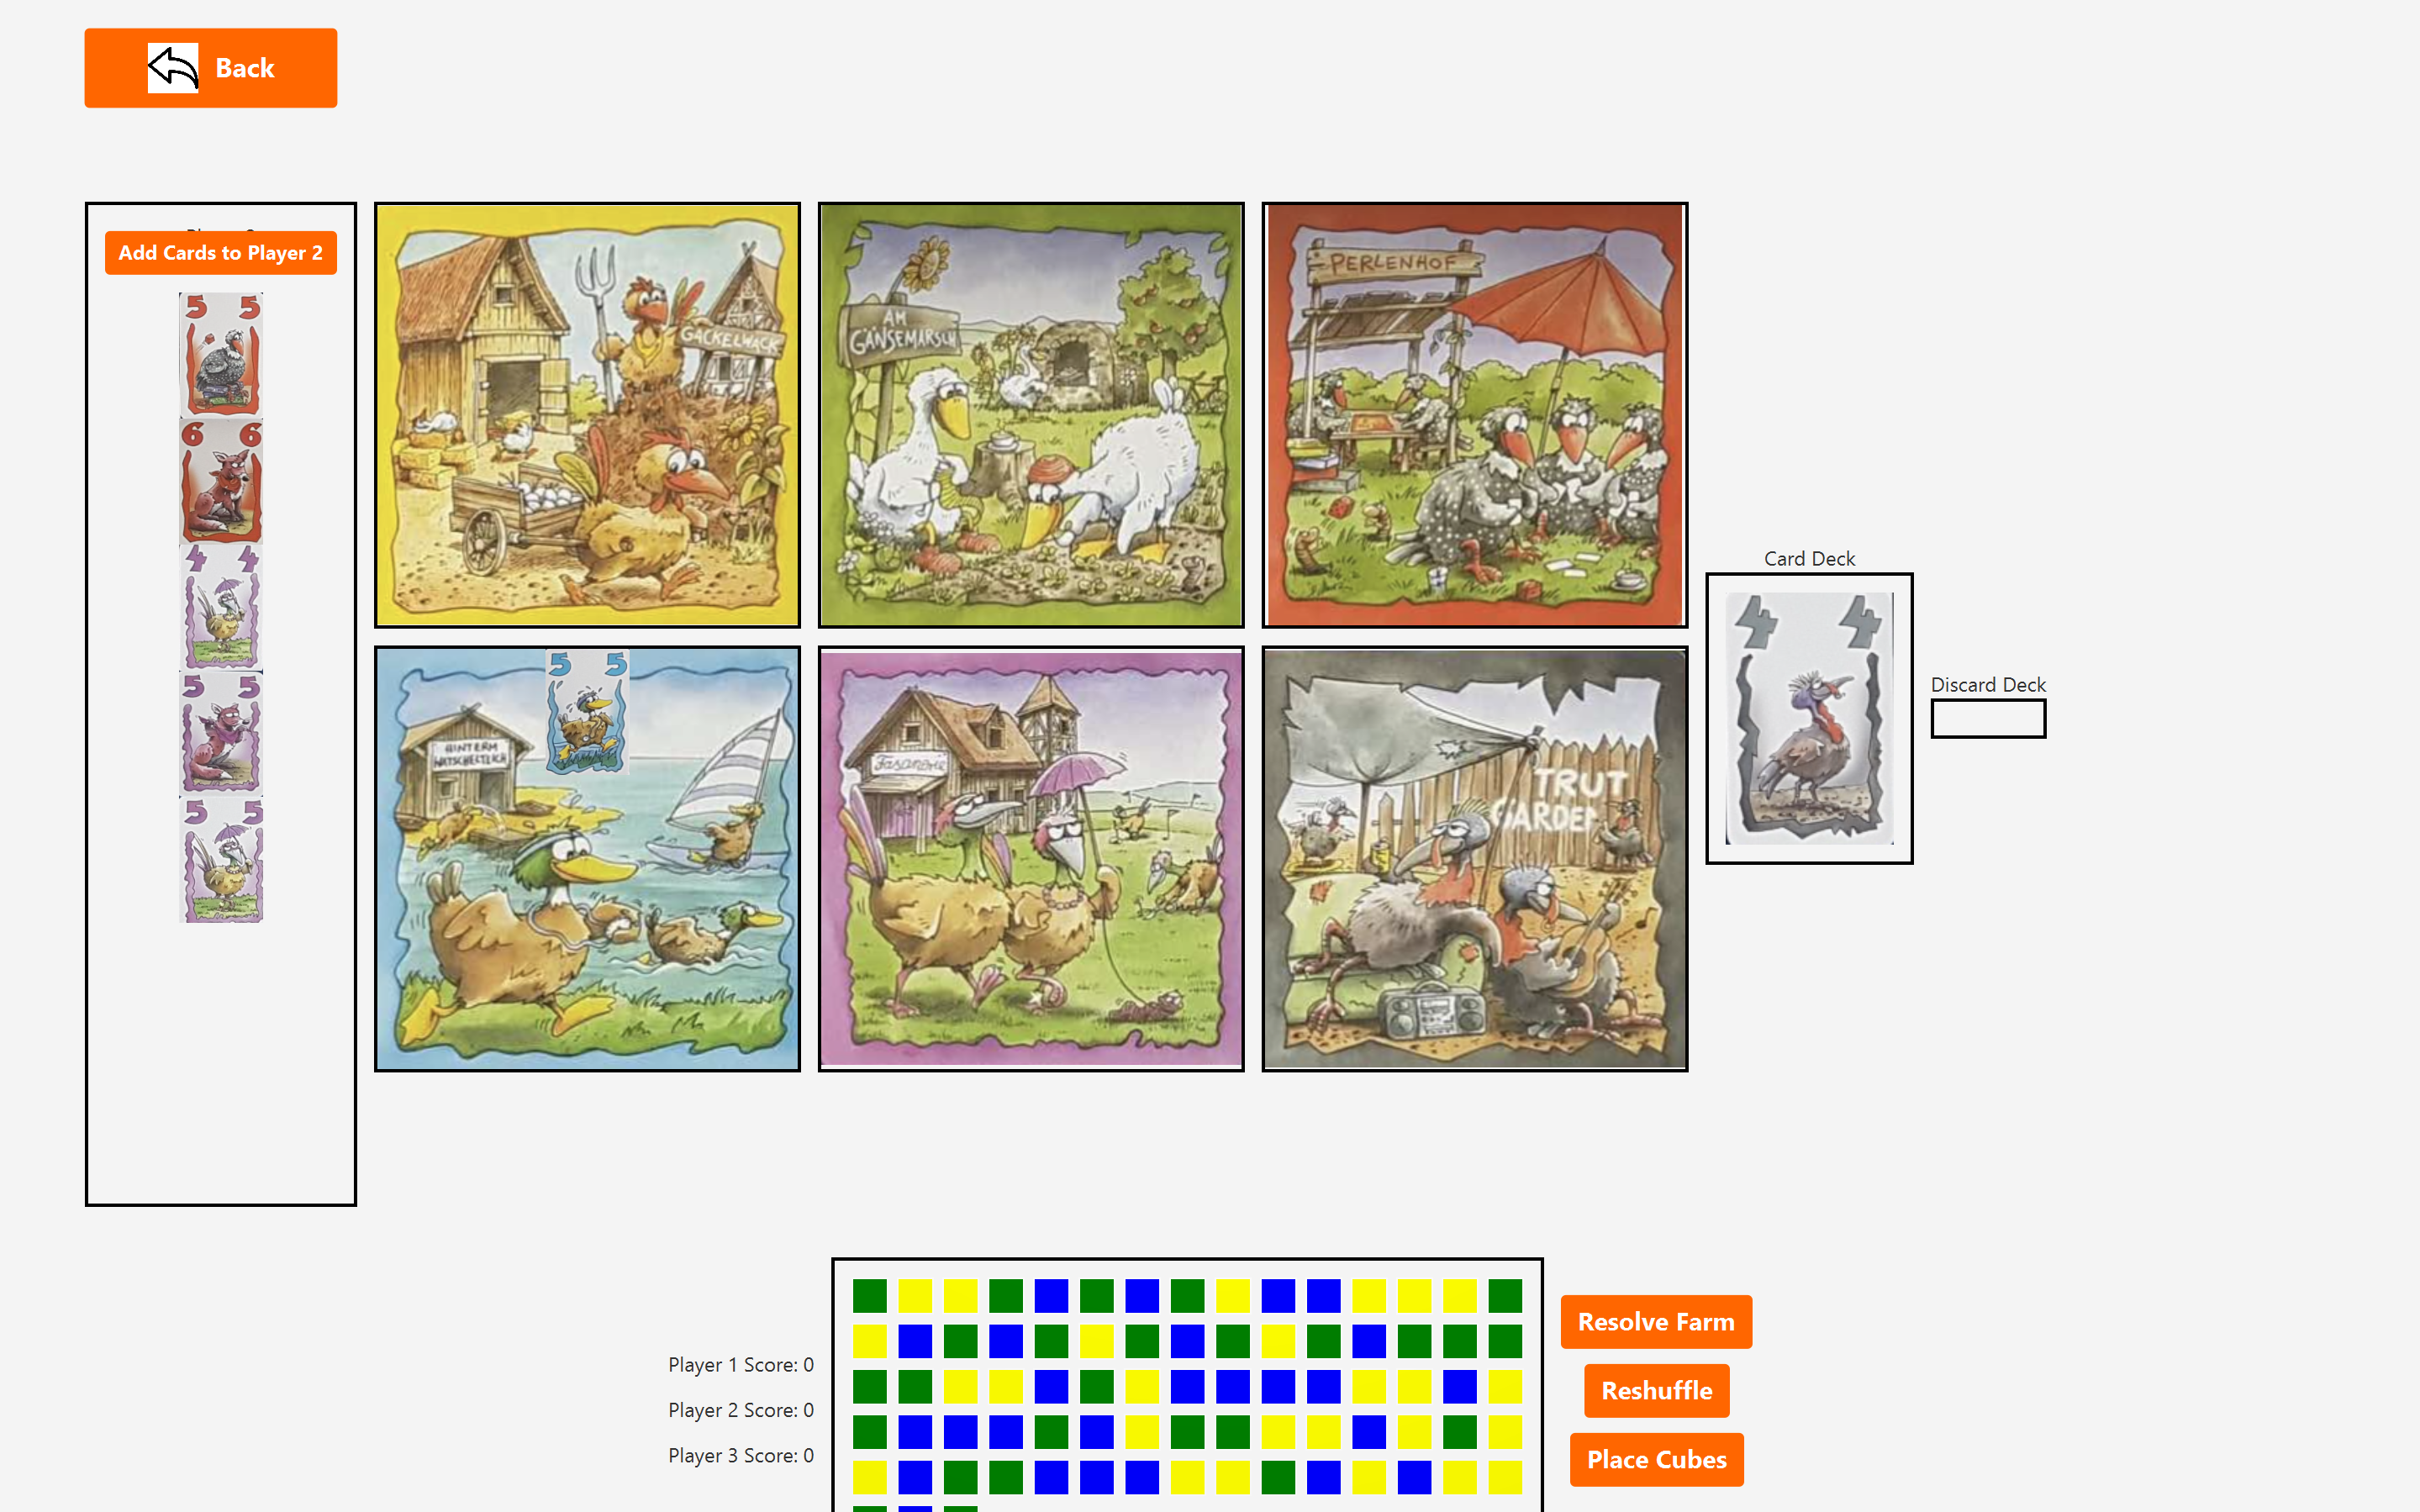
\includegraphics[width=0.5\textwidth]{img/Screenshot 2025-01-14 120420.png} % Adjust the width as needed
    \caption{Game Scene player 2 turn}
    \label{fig:game-scene}
\end{figure} 

\begin{figure}[h!]
    \centering
    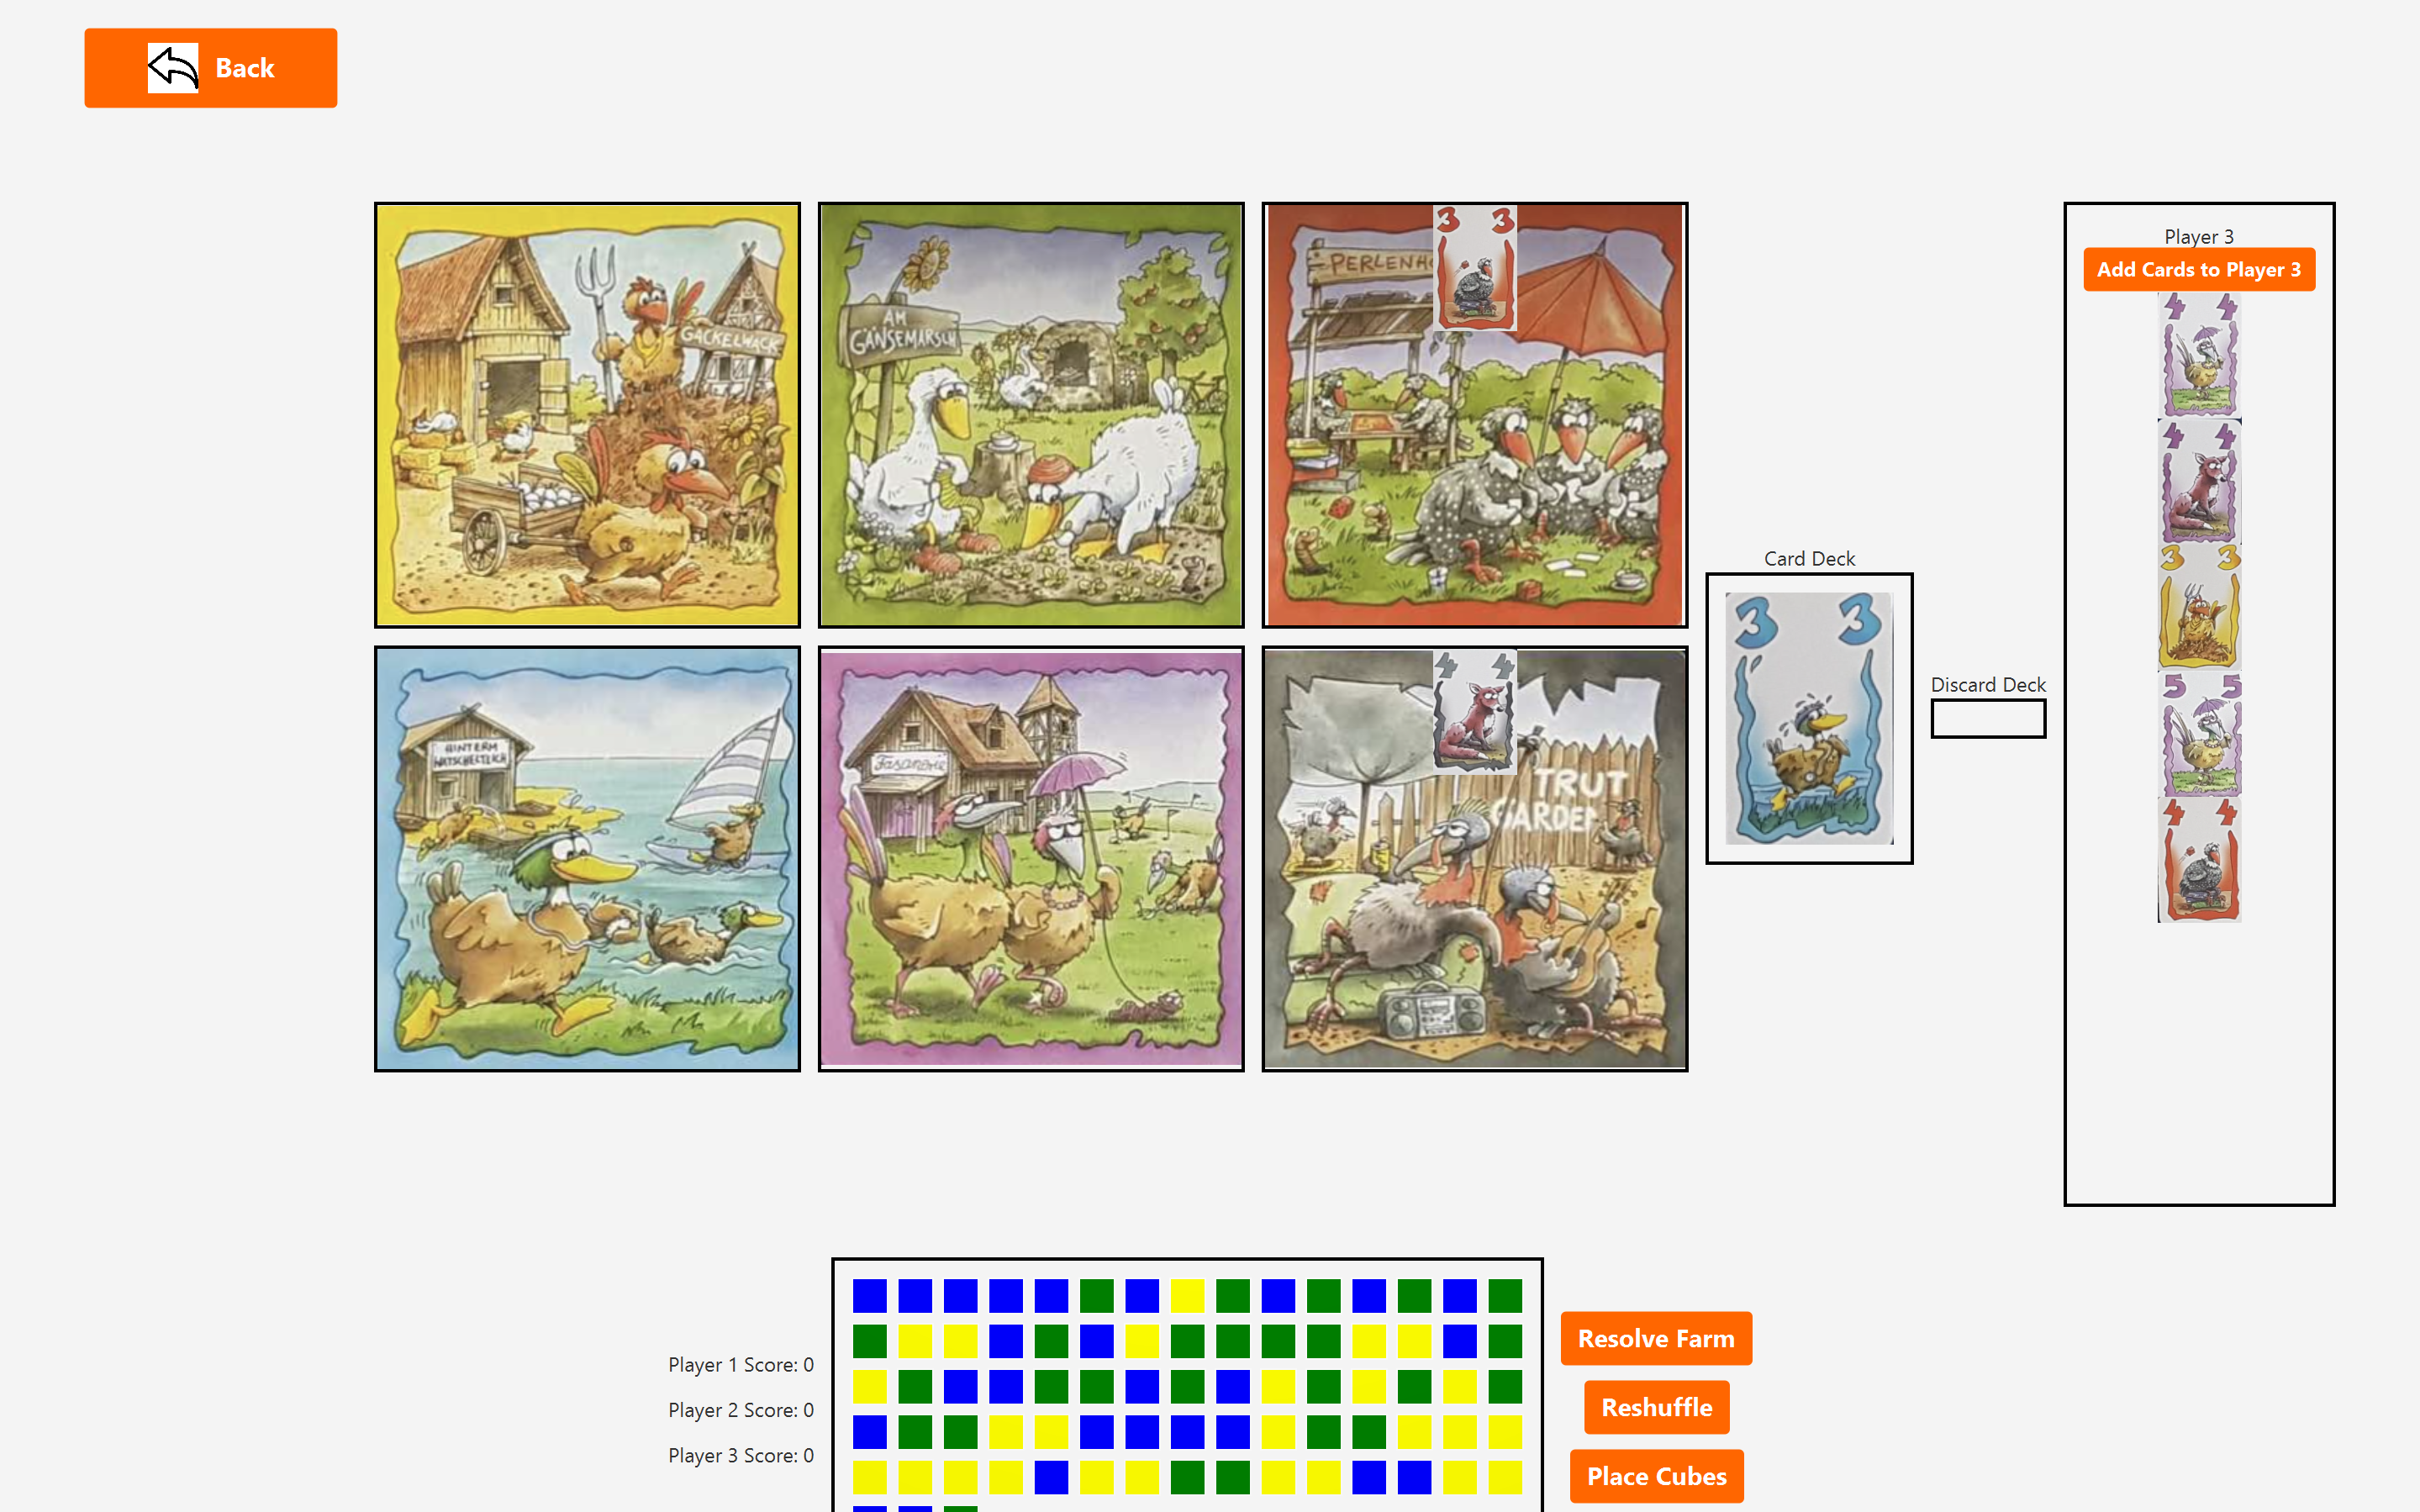
\includegraphics[width=0.5\textwidth]{img/Screenshot 2025-01-14 120632.png} % Adjust the width as needed
    \caption{Game Scene player 3 turn}
    \label{fig:game-scene}
\end{figure} 

\vspace{2cm}

On the top-left, there is a back button, which if players enter this button, the game returns back to the intro scene. There is also image that decorates the back button.

\begin{lstlisting}[language = FXMl, caption = Back Button,basicstyle=\scriptsize, frame=single, framesep=1pt, framerule=0.5pt, xleftmargin=8pt, xrightmargin=8pt]
    @FXML
    private void handleBackToStartAction(ActionEvent event) {
        try {
            // Load the begin.fxml file
            FXMLLoader loader = new FXMLLoader(getClass().getResource("/hellofx/resources/begin.fxml"));
            Parent root = loader.load();

            // Get the controller and set the mainApp reference
            BeginController beginController = loader.getController();
            beginController.setMainApp(mainApp);

            // Get the current stage
            Stage stage = (Stage) ((Button) event.getSource()).getScene().getWindow();

            // Set the new scene
            stage.setScene(new Scene(root));
            stage.setFullScreen(true); // Maximize the stage instead of setting it to full screen
            stage.show();
        } catch (Exception e) {
            e.printStackTrace();
        }
    }
    
\end{lstlisting}

On the top, left, and right of the game, there are players card deck, which in the initial round, players can only see cards of player 1, while player 2 and 3's card decks has been hidden. Inside each player card deck, there are 5 cards, corresponding to the game rule that each player must have 5 cards to start the game. There are also button at each card deck to add a new card to player to keep playing the game.

\begin{figure}[h!]
    \centering
    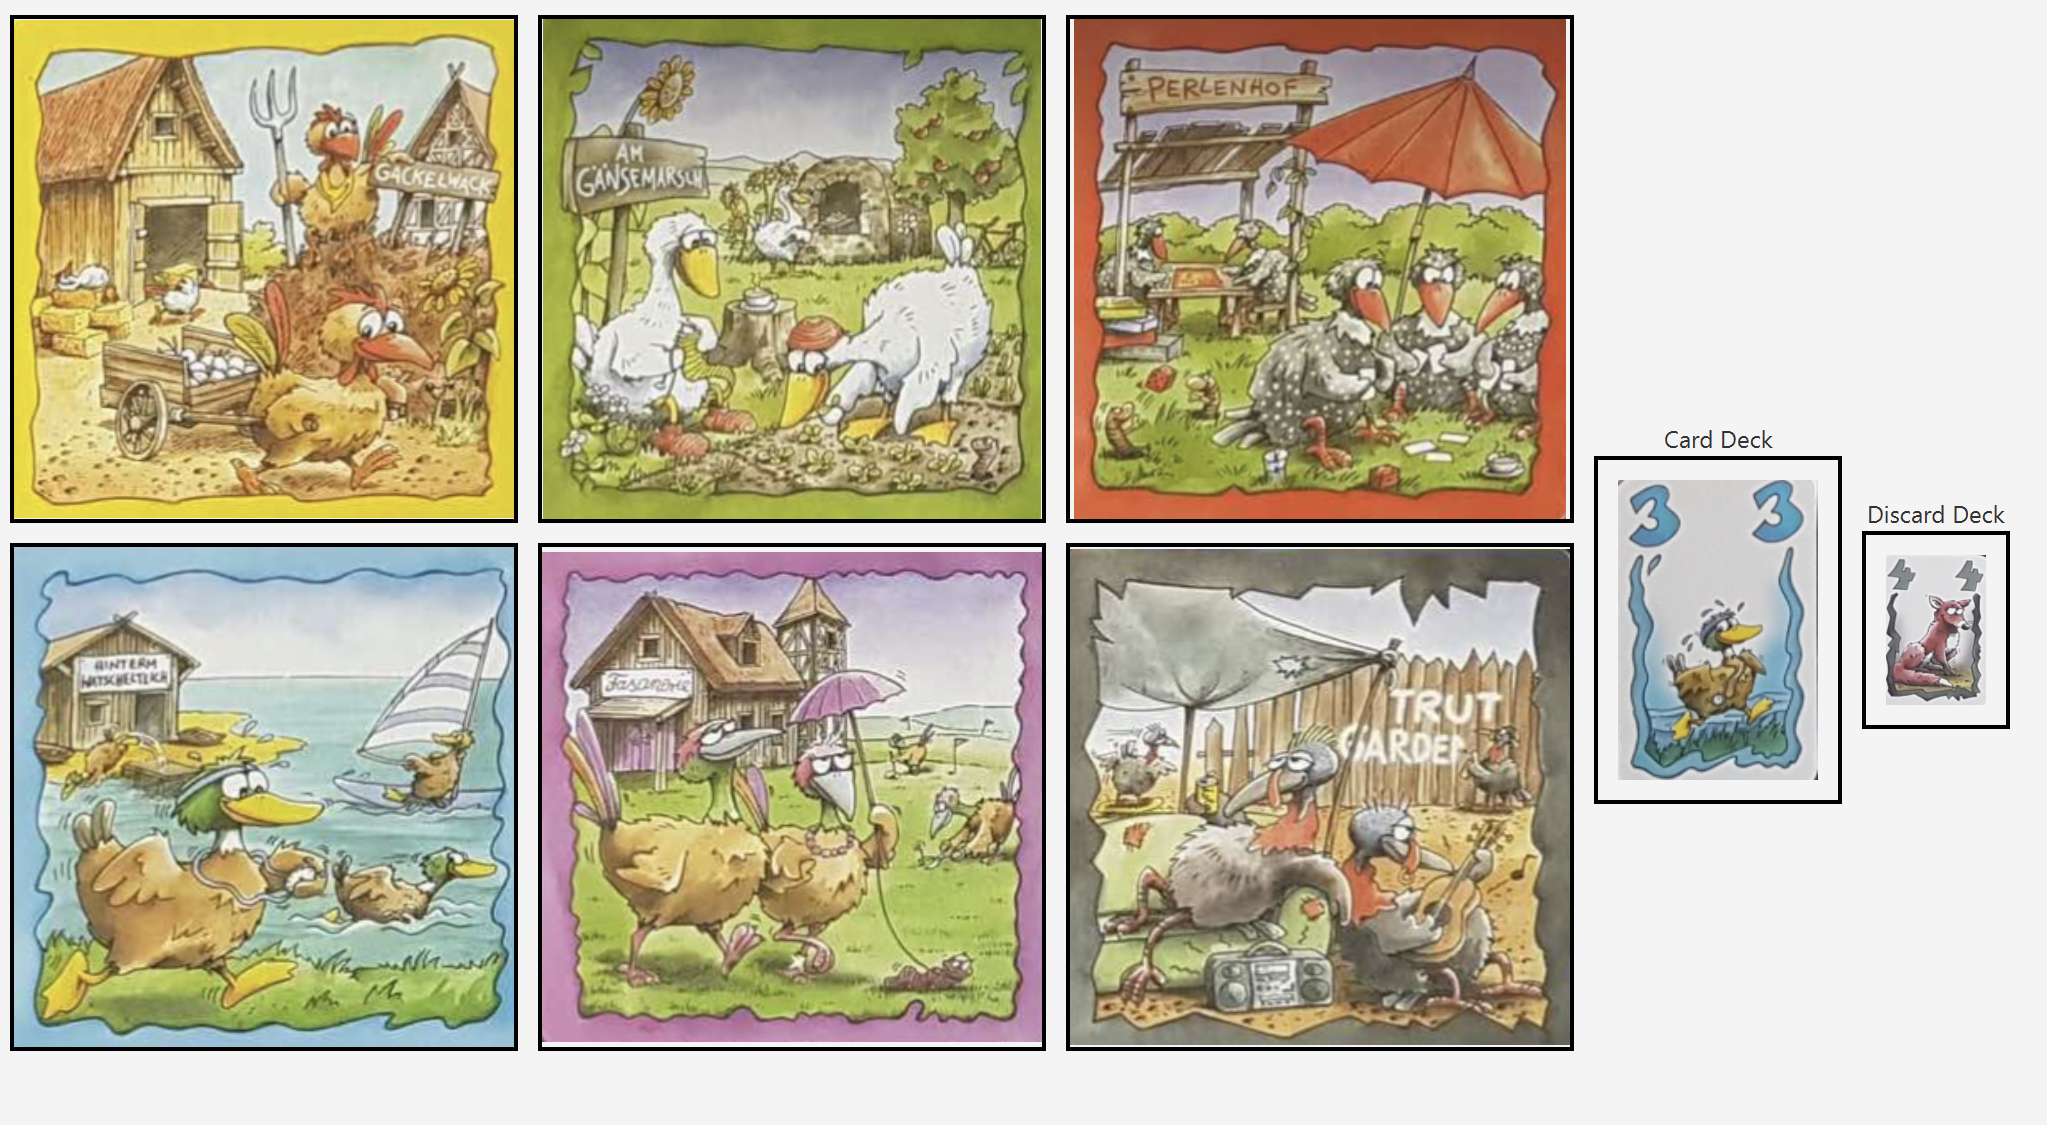
\includegraphics[width=0.5\textwidth]{img/Screenshot 2025-01-14 120930.png} % Adjust the width as needed
    \caption{Center Game Scene}
    \label{fig:use-case-diagram}
\end{figure}

\vspace{0.5cm}

In the center, there are 6 squares, which represent 6 farms for the cards to be placed into. 
Besides, there are 2 decks, which on the left side is the deck containing the main card deck to be added to players' card deck. On the right side is the discard deck, which contains the used cards to play again when there are no cards left in the main card deck.

On the bottom, there is a big box, which contains the available corn cubes, which will be added by clicking the \textbf{Place Cubes} button. At the end of the card and cube addition phase, click \textbf{ resolve farm farm} button to calculate players' score after each turn. When there are no cards left in the main card deck, click the \textbf{Reshuffle} button to reshuffle the discard deck, and it automatically adds back to the main card deck to continue the process.

\vspace{0.5cm}

\begin{figure}[h!]
    \centering
    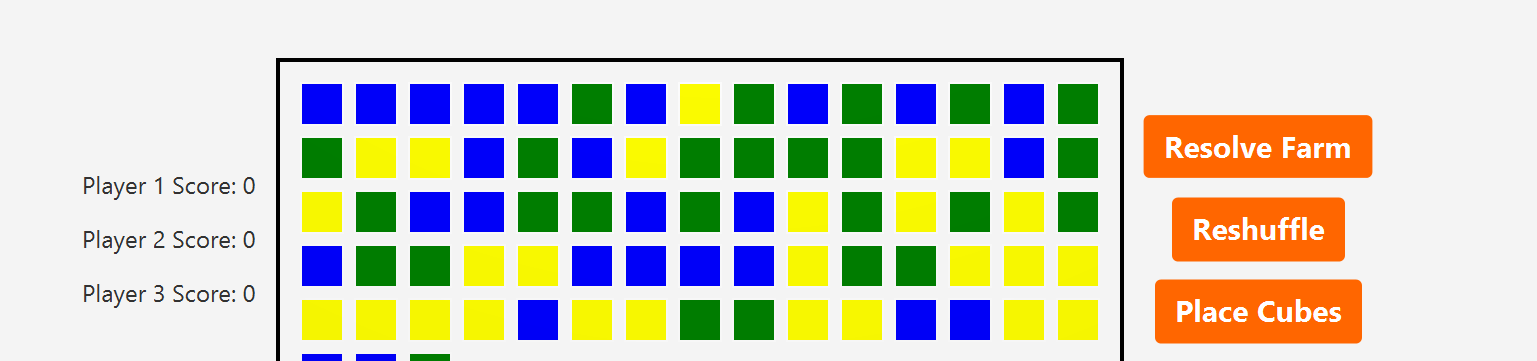
\includegraphics[width=0.5\textwidth]{img/Screenshot 2025-01-14 121133.png} % Adjust the width as needed
    \caption{Bottom Game Scene}
    \label{fig:use-case-diagram}
\end{figure}



\vspace{0.5cm}



\vspace{0.5cm}

\textbf{Winner Scene:}
Here is the winner scene of the game

At the end, when there are no corns left in the corn box, press the \textbf{Resolve Farm} button once more to transition to the winner scene. Here finalize and give congratulations animation to three players with their 3 scores. There are 2 buttons in the winner scene: 


\begin{itemize}
    \item Press the \textbf{Play Again} button to transition back to the intro scene to start a new game.
    \item PRess the \textbf{Exit} button to exit the current game.
\end{itemize}

\begin{figure}
    \centering
    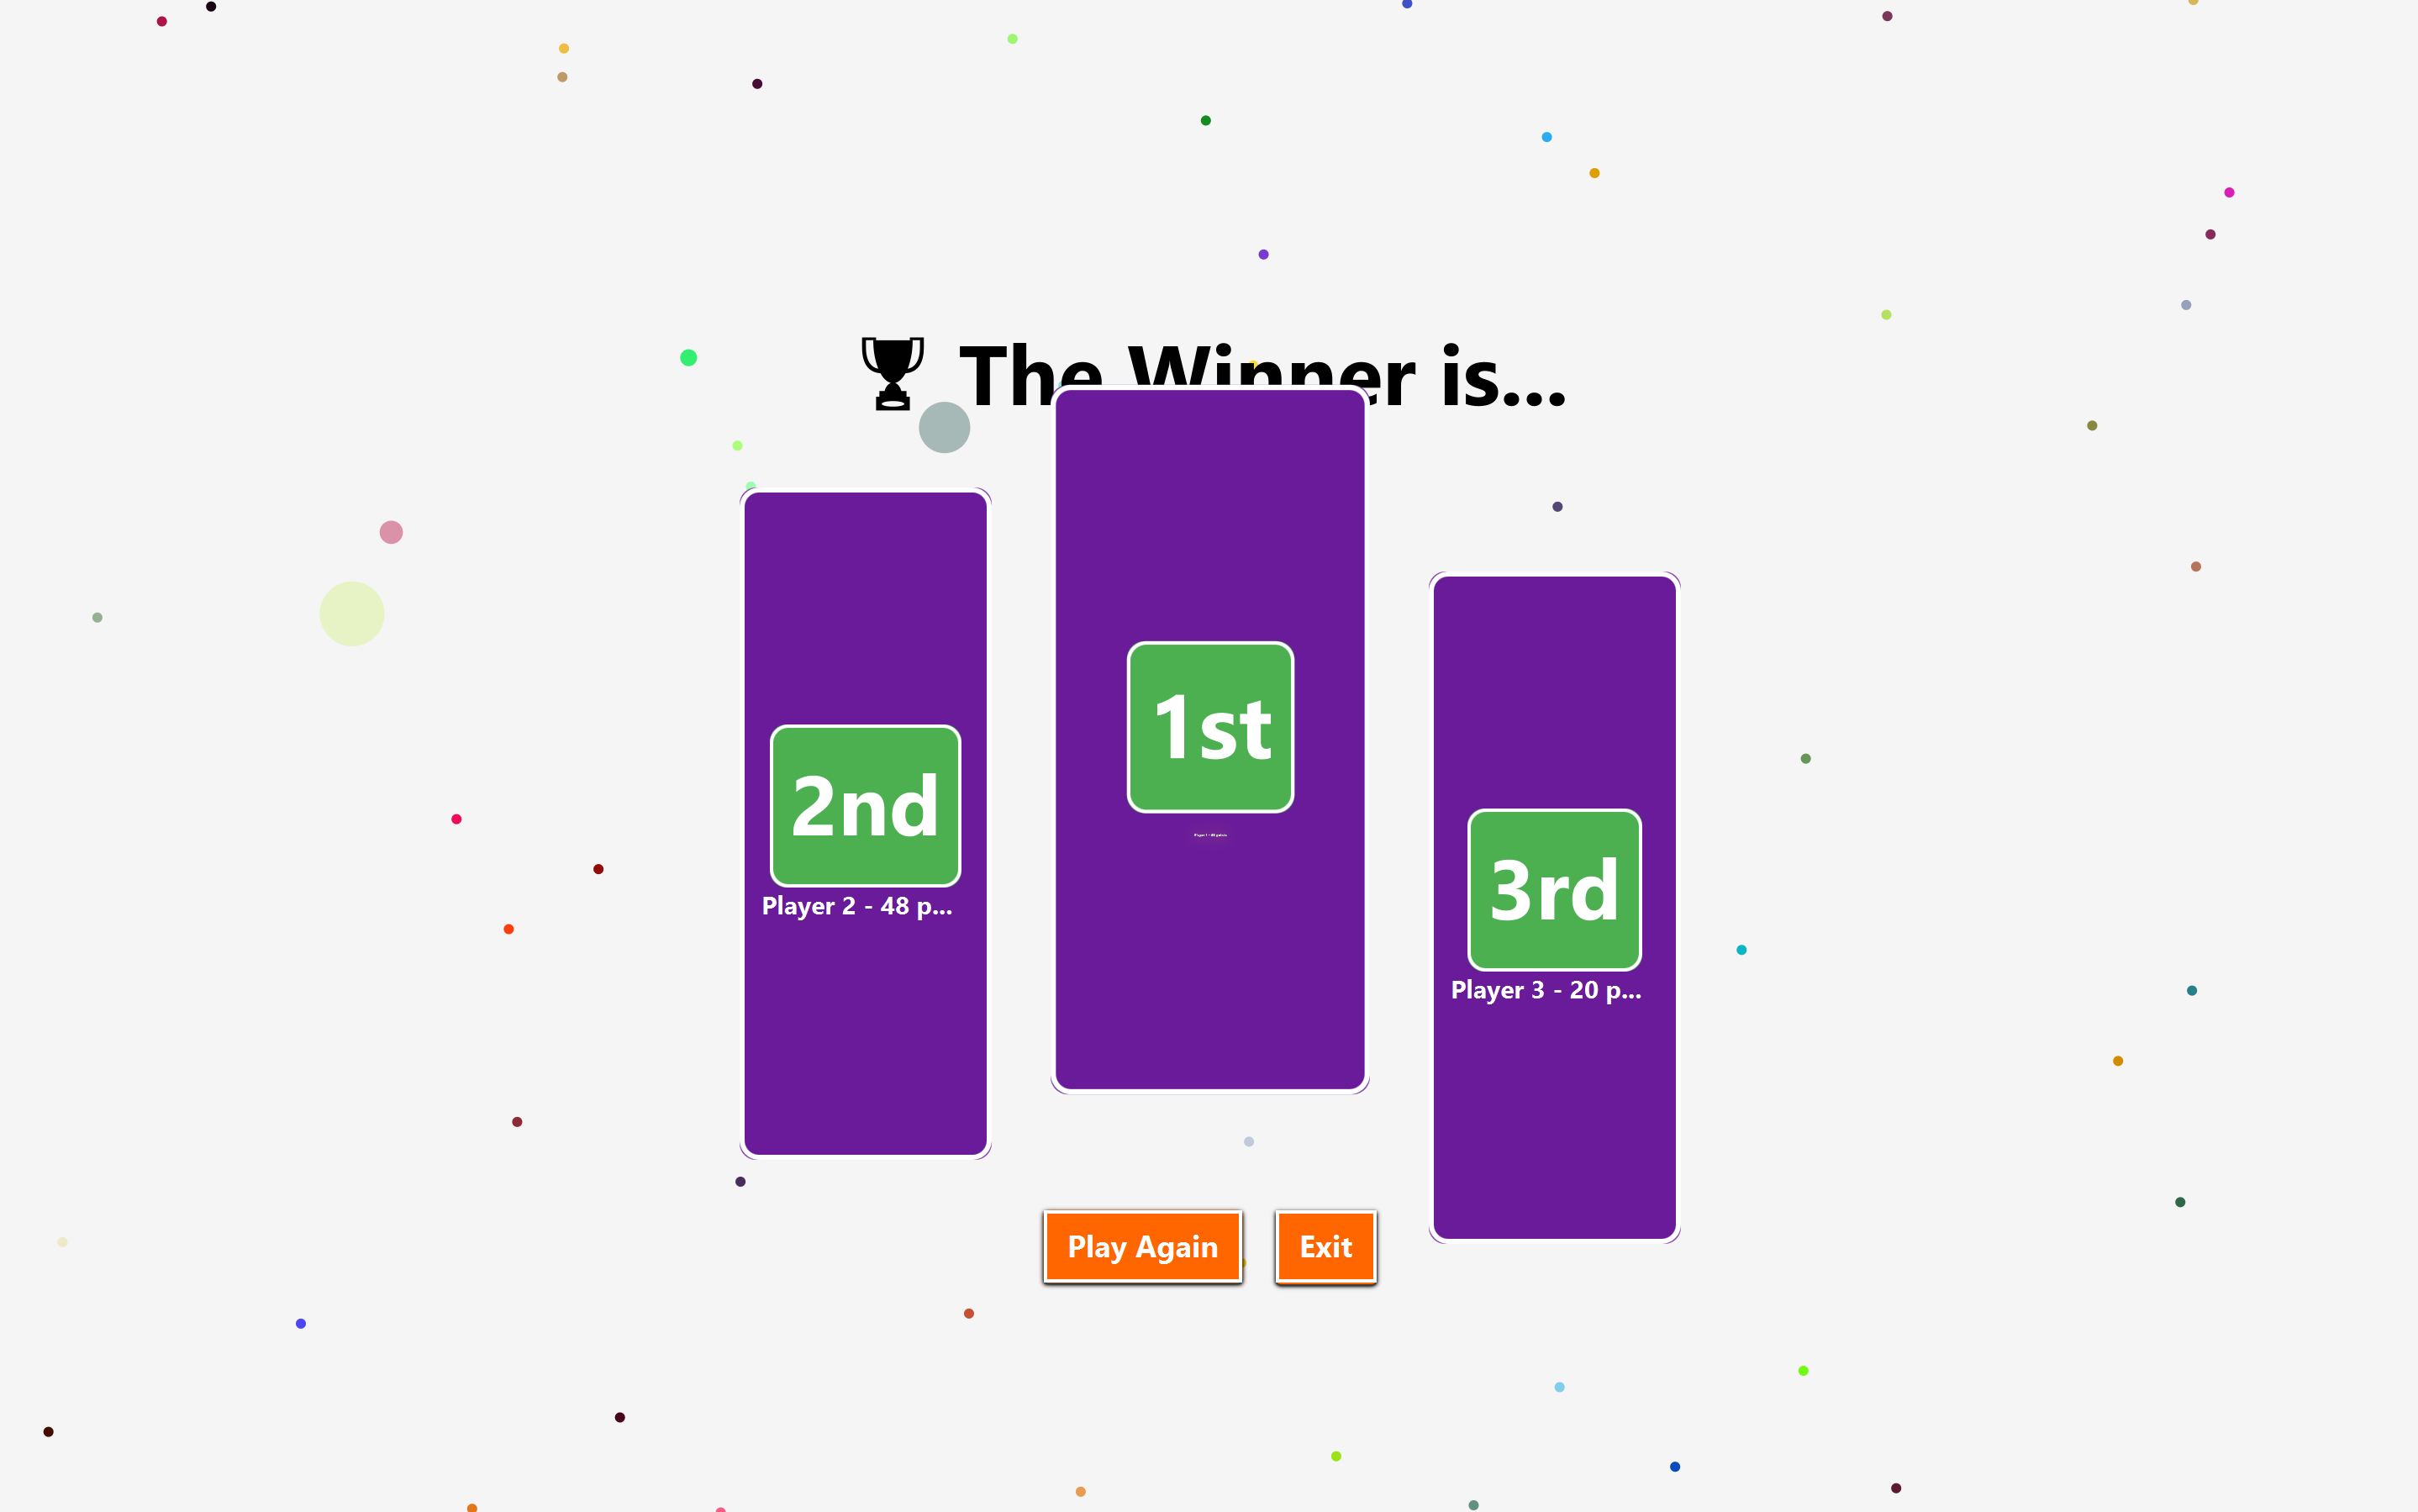
\includegraphics[width=0.5\textwidth]{img/Screenshot 2025-01-14 122727.png} % Adjust the width as needed
    \caption{Winner Scene}
    \label{fig:winner-scene}
\end{figure}

\newpage

\subsection{UML Diagram}

\subsubsection{Class Diagram}



The Class diagram illustrates 6 different classes involved in out Hick Hack boardgame, with those being: Card, Player, Game, CornCube, Farm and Die.

\textbf{Classes:}

\begin{itemize}
    \item Card: includes attributes such as type, value and color to identify each card. Has methods to gets these information and check if it is a fleeing bird.
    \item Player: has a name, a hand of cards and a score pile. Functions include getters, add cards, calculate scores, add to scores and print score.
    \item Game: possesses a list of farms, list of players, a deck, a discard pile and a die. Includes a number of functions for initializing the game and its components, for resolving the farms, for printing out the game state after each round and lastly, declare the winner.
    \item Corncube: each has a color along with methods to get point and get type.
    \item Farm: associates with a distinct color and includes a list of corncubes inside. Uses functions to add and clear corn, get the color and the list of corncubes.
    \item Die: attributes include a value and a method to roll.
\end{itemize}

\textbf{Relationships:}

\begin{itemize}
    \item Player - Card: since each player has a 5 cards on hand and each card only belongs to 1 player at a time, it is therefore a 1:N relationship.
    \item Game - Card: a game has a total of 60 cards and each card is only in 1 game, so the relationship is 1:N as well.
    \item Game - Player: this is a 1:N association because a game has a number of players but a player only play 1 game at a time.
    \item Game - Farm: A game contains 6 farms and each farm only goes with a single game, so the relationship is 1:N.
    \item Game - Die: A game only as 1 die and a die is used only in that game, hence it is a 1:1 association.
    \item Farm - Corncube: a farm may contain any number of cubes but a cube is only contained in 1 farm, therefore, it is a 1:N relationship.
\end{itemize}

\begin{figure}[h!]
    \centering
    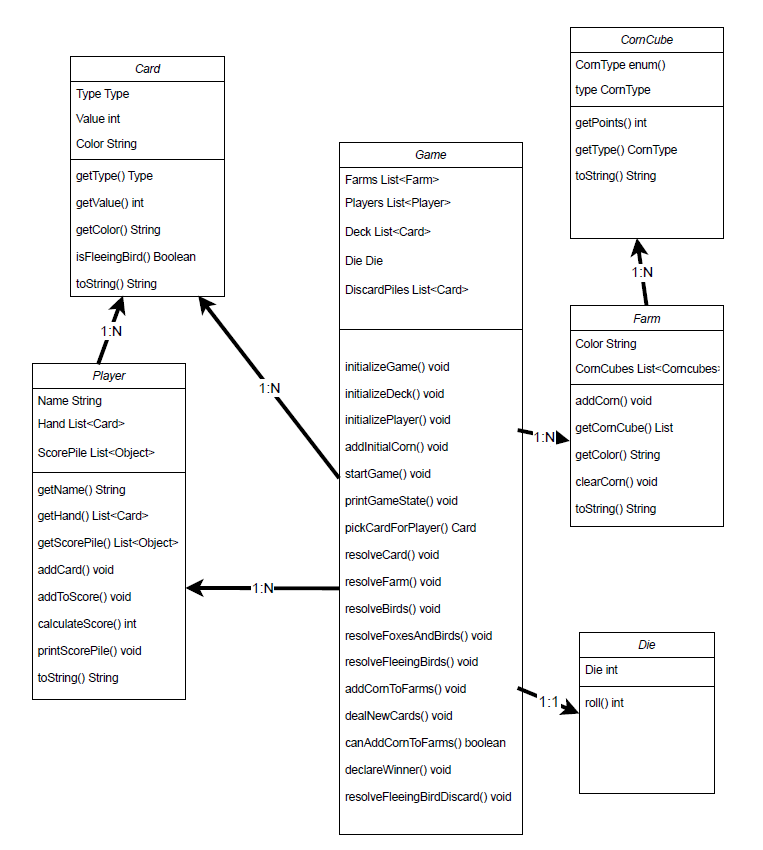
\includegraphics[width=0.5\textwidth]{img/Class Diagram.png} % Adjust the width as needed
    \caption{Class Diagram}
    \label{fig:class-diagram}
\end{figure}

% \newpage

\subsubsection{Use Case Diagram}



The Use Case diagram demonstrates a number of actors and their use cases involved in the Hick Hack boardgame. The primary actor is the Game and secondary actors include CornCube, Farm, Deck, Card, DiscardPile and Player.

\textbf{Main use cases:}

The game begins with Start Game, which initializes essential components like the deck, farms, players, and discard pile. Use cases such as Create Farm, Add Initial Corns, and Create Deck handle the setup by defining farms, distributing corn resources, and preparing cards. During gameplay, players interact with use cases like Place Card, which moves cards to the discard pile, and Resolve Card, which manages the outcomes of actions on farms, birds, foxes, and scores. The diagram also includes tasks for calculating scores and maintaining game progression, ensuring modular and efficient execution.

\textbf{Relationships:}
The relationships in the Use Case diagram showcase a structured and interconnected system where higher-level processes depend on smaller, modular tasks. The primary actor, Game, interacts with most use cases to initiate and manage gameplay, while supporting actors like CornCube, Farm, Deck, Card, DiscardPile, and Player perform specialized roles. Use cases are linked through include and extend relationships, ensuring modularity and reusability. For example, foundational use cases like Create Farm and Create Deck rely on smaller tasks such as Get Card Type or Add Corn Cubes for setup, while gameplay resolutions like Resolve Card extend into specific actions such as Resolve Birds or Add To Score. This interconnected structure ensures a seamless flow of actions while maintaining clarity and flexibility in the system.

\begin{figure}[h!]
    \centering
    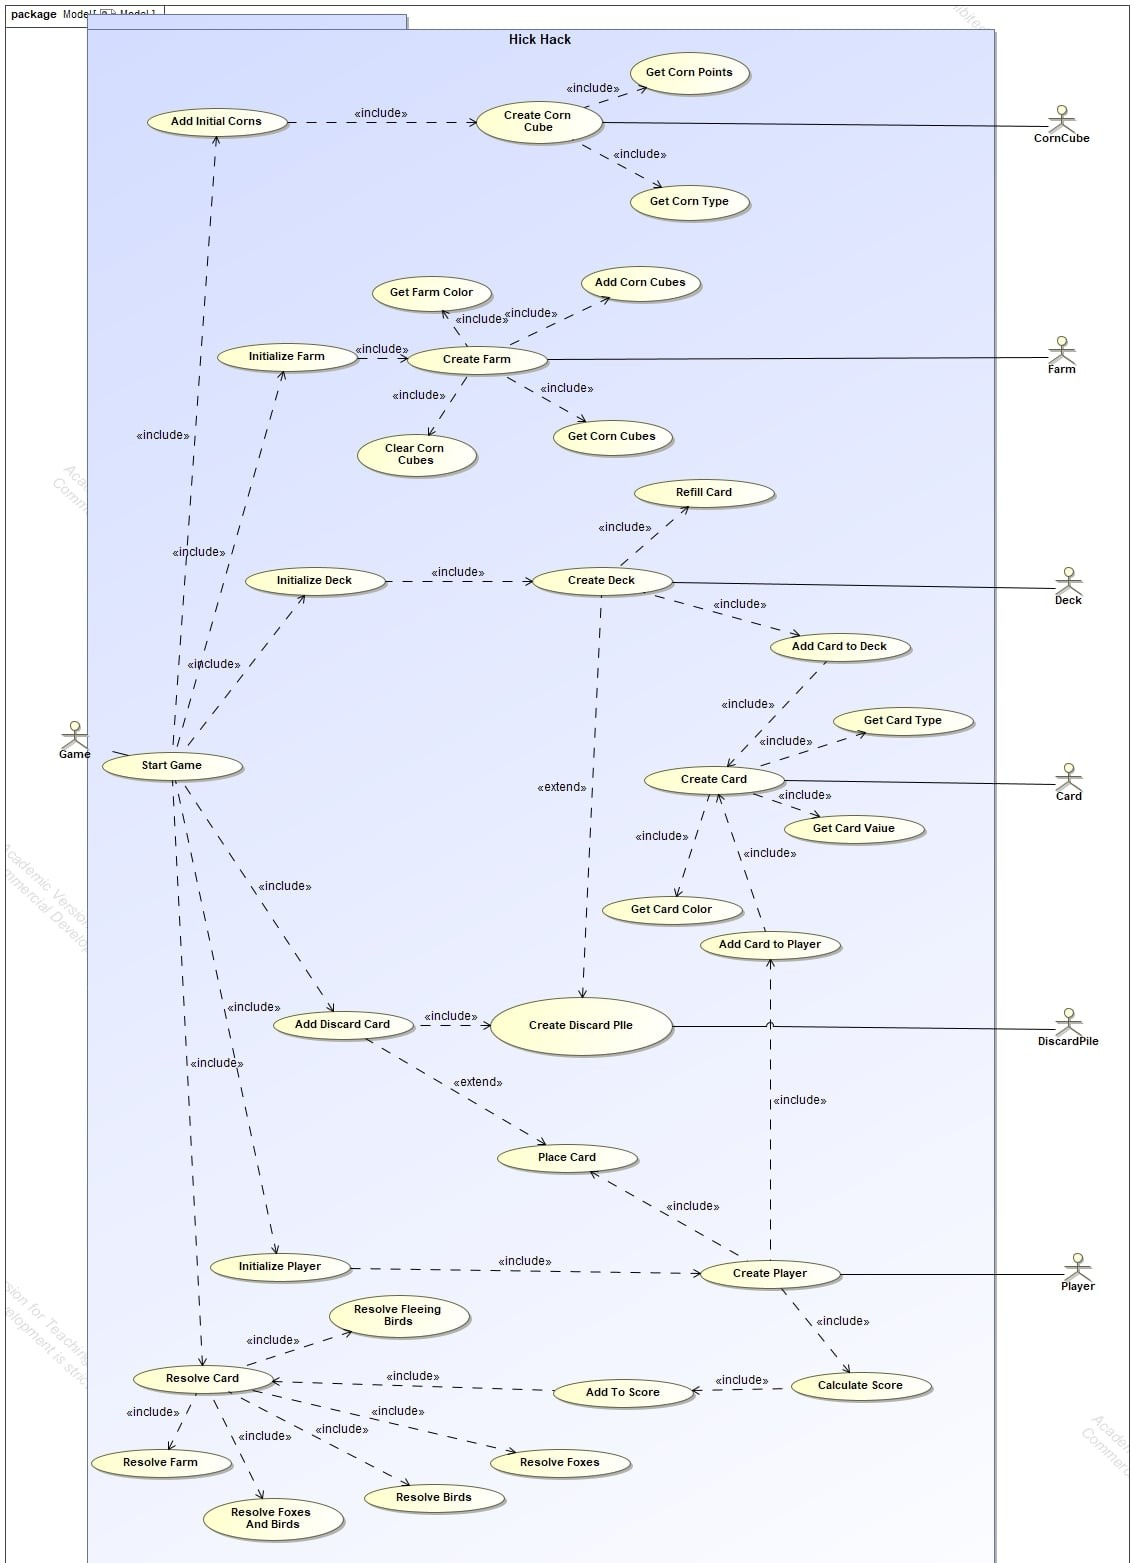
\includegraphics[width=0.48\textwidth]{img/Java Board Game Use Case Diagram.jpeg} % Adjust the width as needed
    \caption{Use Case Diagram}
    \label{fig:use-case-diagram}
\end{figure}


\subsubsection{Sequence Diagram}



The Sequence Diagram illustrates the ordered sequence of actions performed by the Hick Hack game. A total of 7 object lifecycles are shown: Game, Farm, CornCube, Card, Deck, Discard Pile and Player.

\textbf{Sequence:}

\begin{itemize}
    \item The Game starts by initialize the 6 farms, each with a distinct color.
    \item Next, we will initialize the deck by adding cards to it.
    \item Initialize players by adding cards to their hand.
    \item Add a random cube to each farm.
    \item After initialization, the game enters a while loop until there are not enough corn cubes to be added.
    \item Each player choose a card from their hand.
    \item Resolve the cards.
    \item Resolve the farms.
    \item Add played cards to the discard pile.
    \item Display the game state, such as the information regarding the deck, the discard pile, number of corn cubes remaining and each player's score pile.
    \item After each turn, if there are enough cards in the deck, refill each player's hand with 1 card. If not enough, reshuffle the discard pile back to the deck and distribute a card to each player.
    \item Also check if there are enough corn to distribute to each farm for the next turn, if not enough, the game ends and the player with the highest score wins.
\end{itemize}

\begin{figure}[h!]
    \centering
    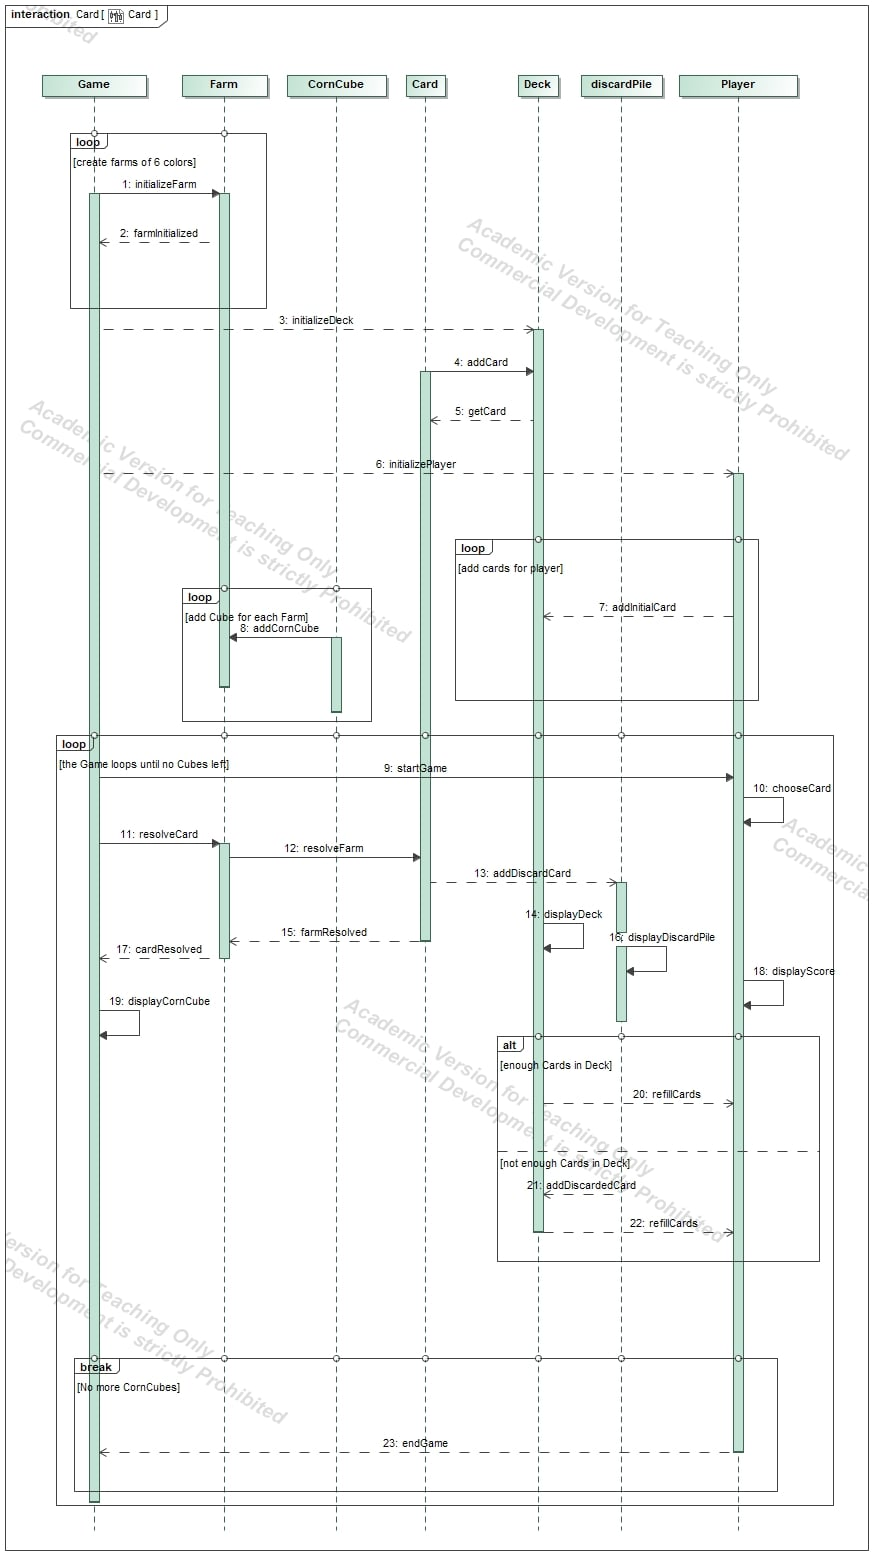
\includegraphics[width=0.5\textwidth]{img/Java Board Game Sequence Diagram.jpeg} % Adjust the width as needed
    \caption{Sequence Diagram}
    \label{fig:sequence-diagram}
\end{figure}


\subsection{Used Libraries}
\begin{itemize}
    \item import javafx.fxml.FXML;
    \item import javafx.fxml.FXMLLoader;
    \item import javafx.geometry.Bounds;
    \item import javafx.geometry.Insets;
    \item import javafx.geometry.Pos;
    \item import javafx.scene.Parent;
    \item import javafx.scene.Scene;
    \item import javafx.scene.control.Button;
    \item import javafx.scene.image.Image;
    \item import javafx.scene.image.ImageView;
    \item import javafx.scene.layout.StackPane;
    \item import javafx.scene.layout.VBox;
    \item import javafx.scene.layout.Background;
    \item import javafx.scene.layout.BackgroundImage;
    \item import javafx.scene.layout.BackgroundPosition;
    \item import javafx.scene.layout.BackgroundRepeat;
    \item import javafx.scene.layout.BackgroundSize;
    \item import javafx.scene.layout.FlowPane;
    \item import javafx.scene.layout.GridPane;
    \item import javafx.scene.layout.Pane;
    \item import javafx.scene.control.Label;
    \item import javafx.scene.paint.Color;
    \item import javafx.scene.shape.Box;

    \item import javafx.stage.Stage;
    \item import javafx.scene.paint.PhongMaterial;
    \item import javafx.animation.KeyFrame;
    \item import javafx.animation.KeyValue;
    \item import javafx.animation.Timeline;
    \item import javafx.animation.TranslateTransition;
    \item import javafx.event.ActionEvent;
    \item import javafx.util.Duration;


    \item import java.util.Iterator;
    \item import java.io.FileInputStream;
    \item import java.io.FileNotFoundException;
    \item import java.io.InputStream;
    \item import java.util.ArrayList;
    \item import java.util.Arrays;
    \item import java.util.Collections;
    \item import java.util.HashMap;
    \item import java.util.List;
    \item import java.util.Map;
    \item import java.util.Random;
    \item import java.util.stream.Collectors;
    \item import javafx.animation.*
\end{itemize}

\subsection{Code Snippets}
Here represents the codes to calculate player score.
\begin{itemize}
    \item Case 1: When there is one unique card in a farm
    \begin{figure}[h!]
        \centering
        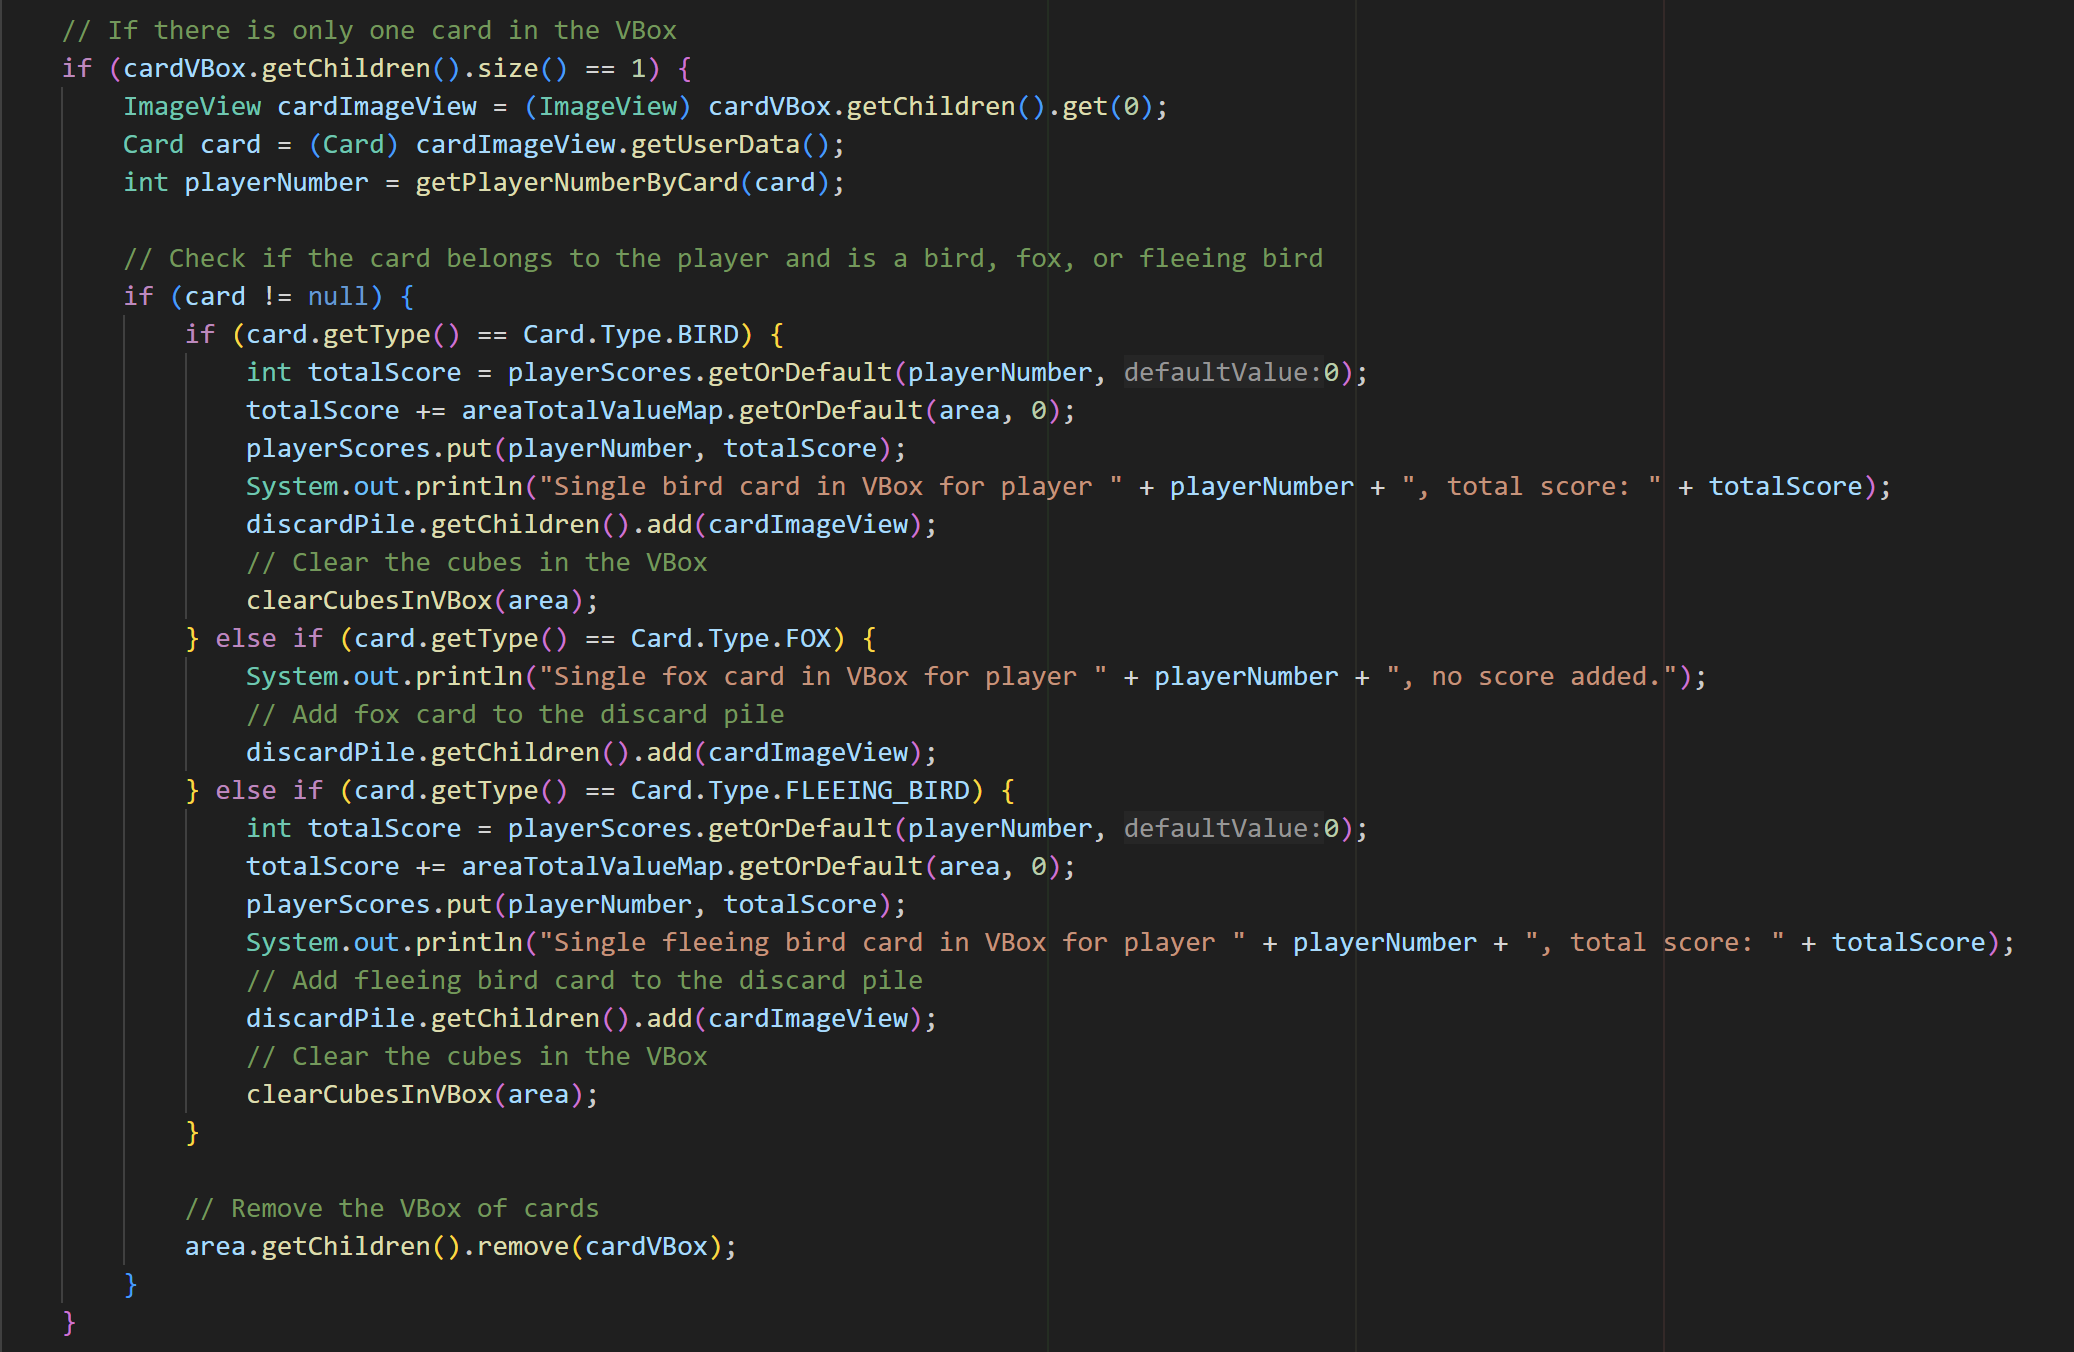
\includegraphics[width=0.5\textwidth]{img/Screenshot 2025-01-14 125602.png} % Adjust the width as needed
        \caption{Case 1}
        \label{fig:case}
    \end{figure}

    \vspace{6.5cm}
    \item Case 2: When there are 2 birds in a farm
    \begin{figure}[h!]
        \centering
        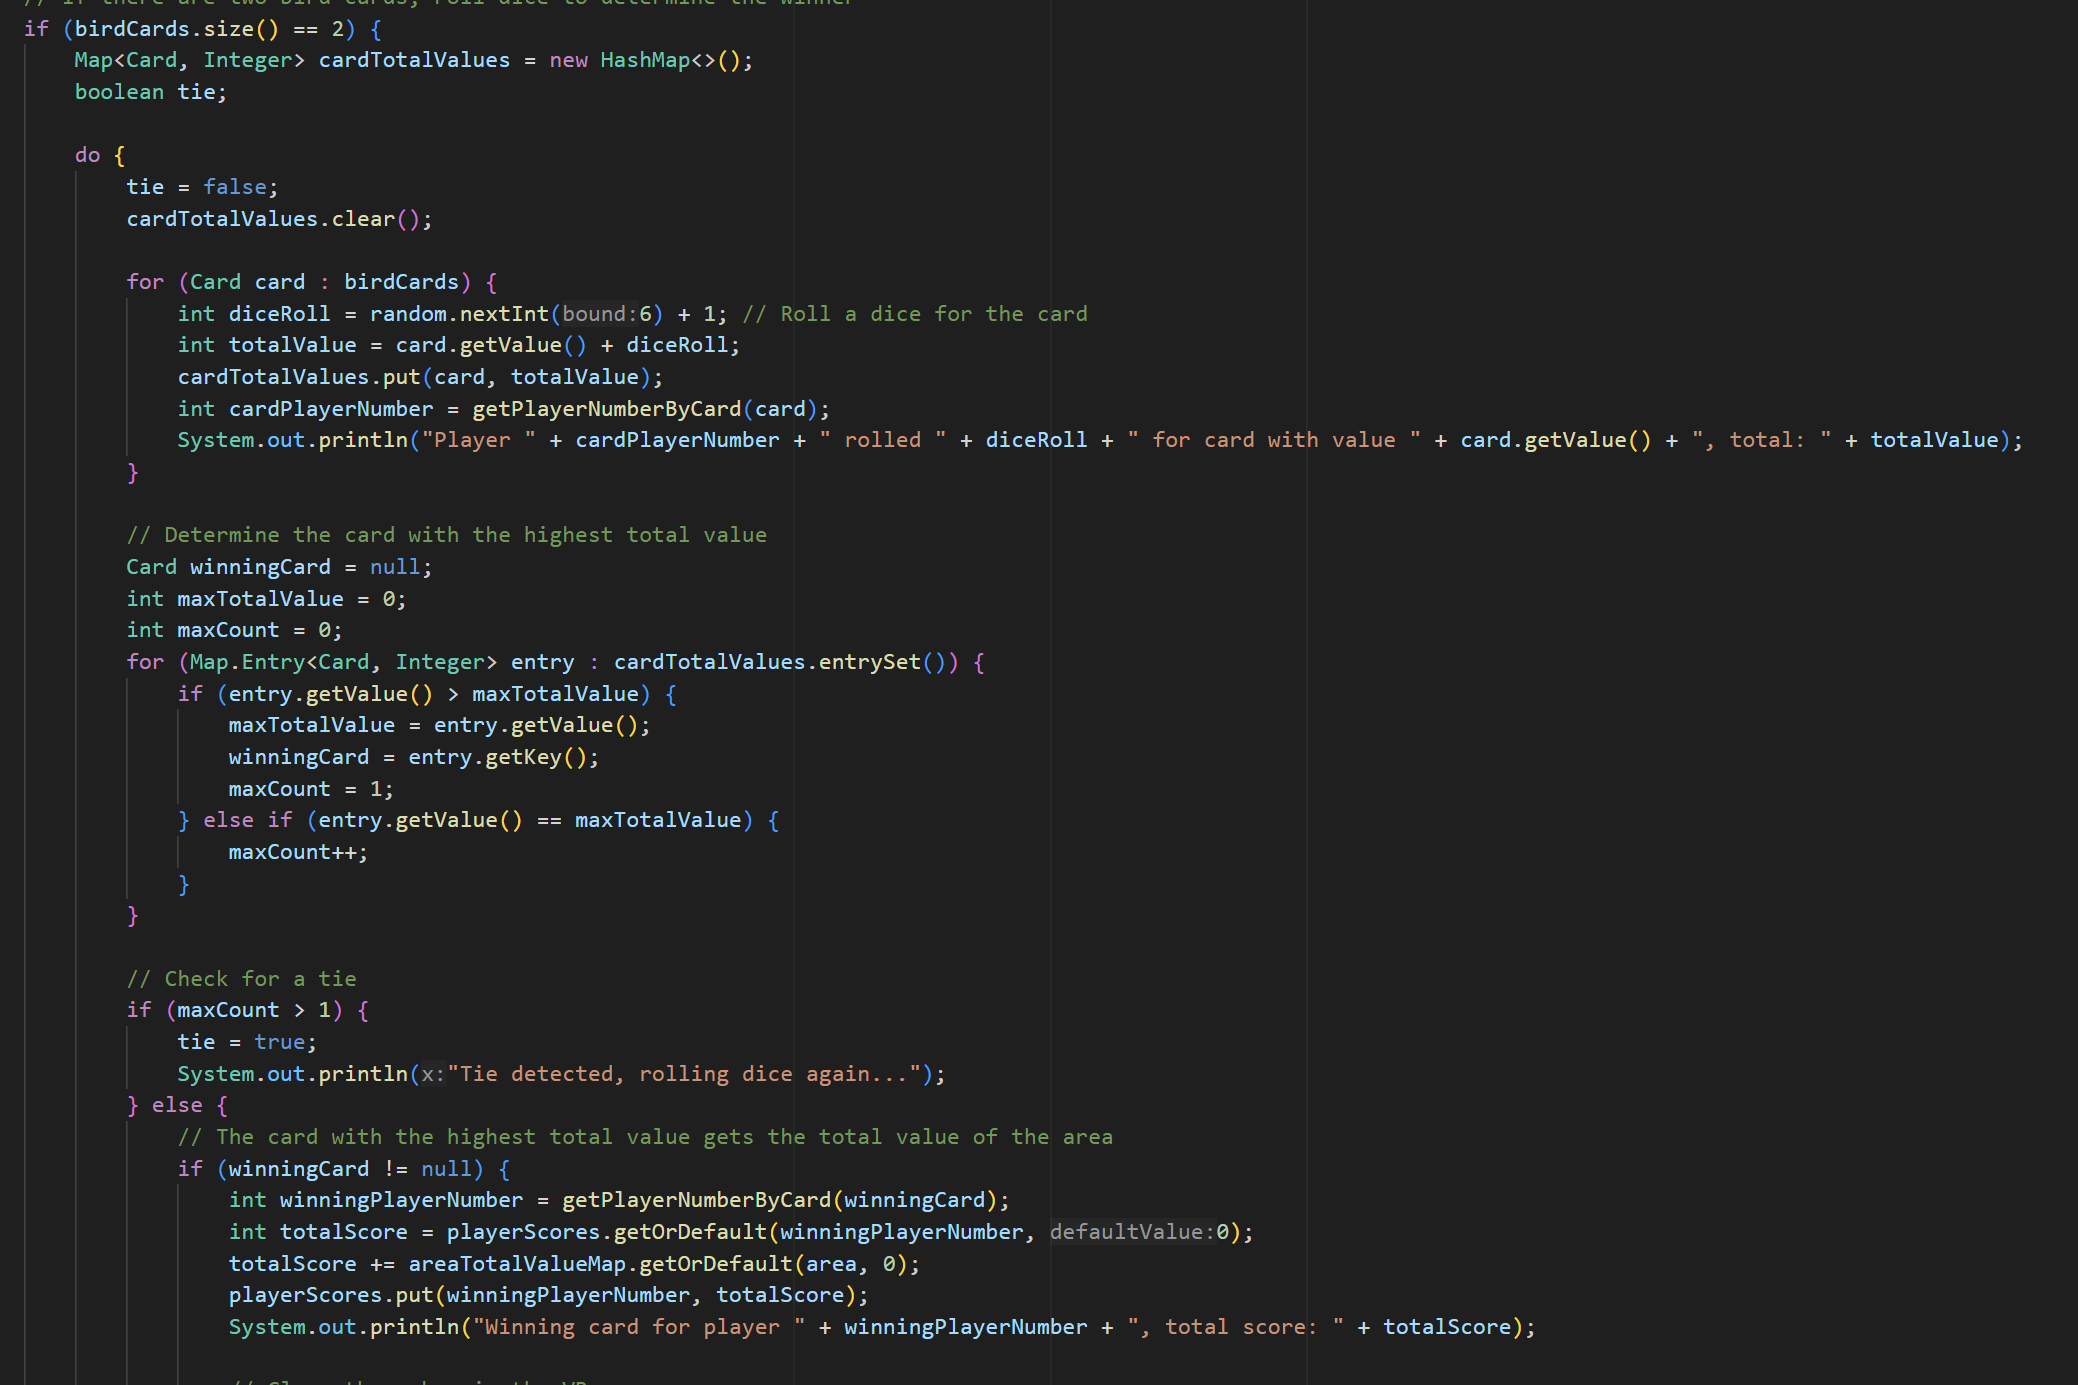
\includegraphics[width=0.5\textwidth]{img/Screenshot 2025-01-14 125854.png} % Adjust the width as needed
        \caption{Case 2}
        \label{fig:case}
    \end{figure}
    \item Case 3: When there are 2 foxes in a farm
    \vspace{0.1cm}
    \begin{figure}[h!]
        \centering
        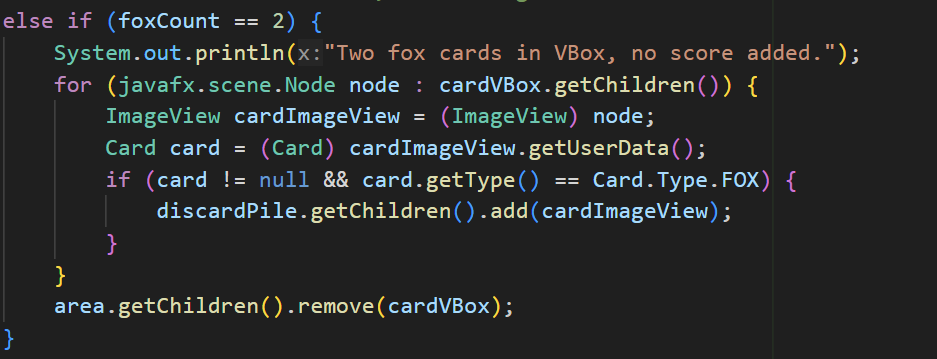
\includegraphics[width=0.5\textwidth]{img/Screenshot 2025-01-14 130028.png} % Adjust the width as needed
        \caption{Case 3}
        \label{fig:case}
    \end{figure}
    \vspace{1cm}
    \item Case 4: When there are 1 bird and 1 fleeing bird
    \begin{figure}[h!]
        \centering
        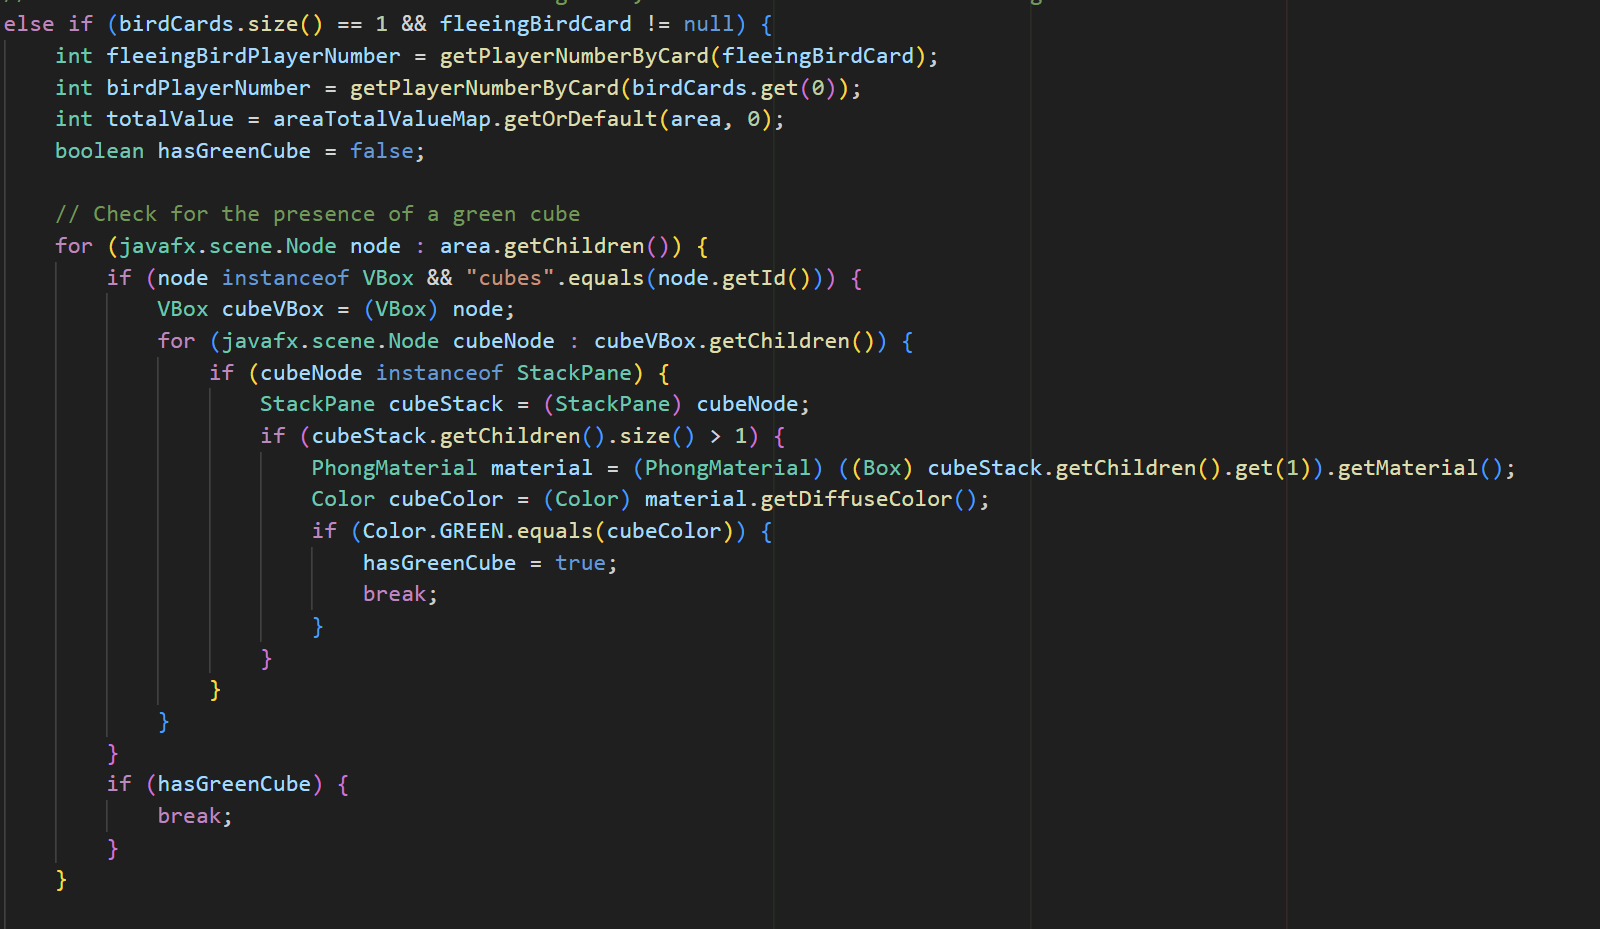
\includegraphics[width=0.5\textwidth]{img/Screenshot 2025-01-14 130113.png} % Adjust the width as needed
        \caption{Case 4}
        \label{fig:case}
    \end{figure}
    \begin{figure}[h!]
        \centering
        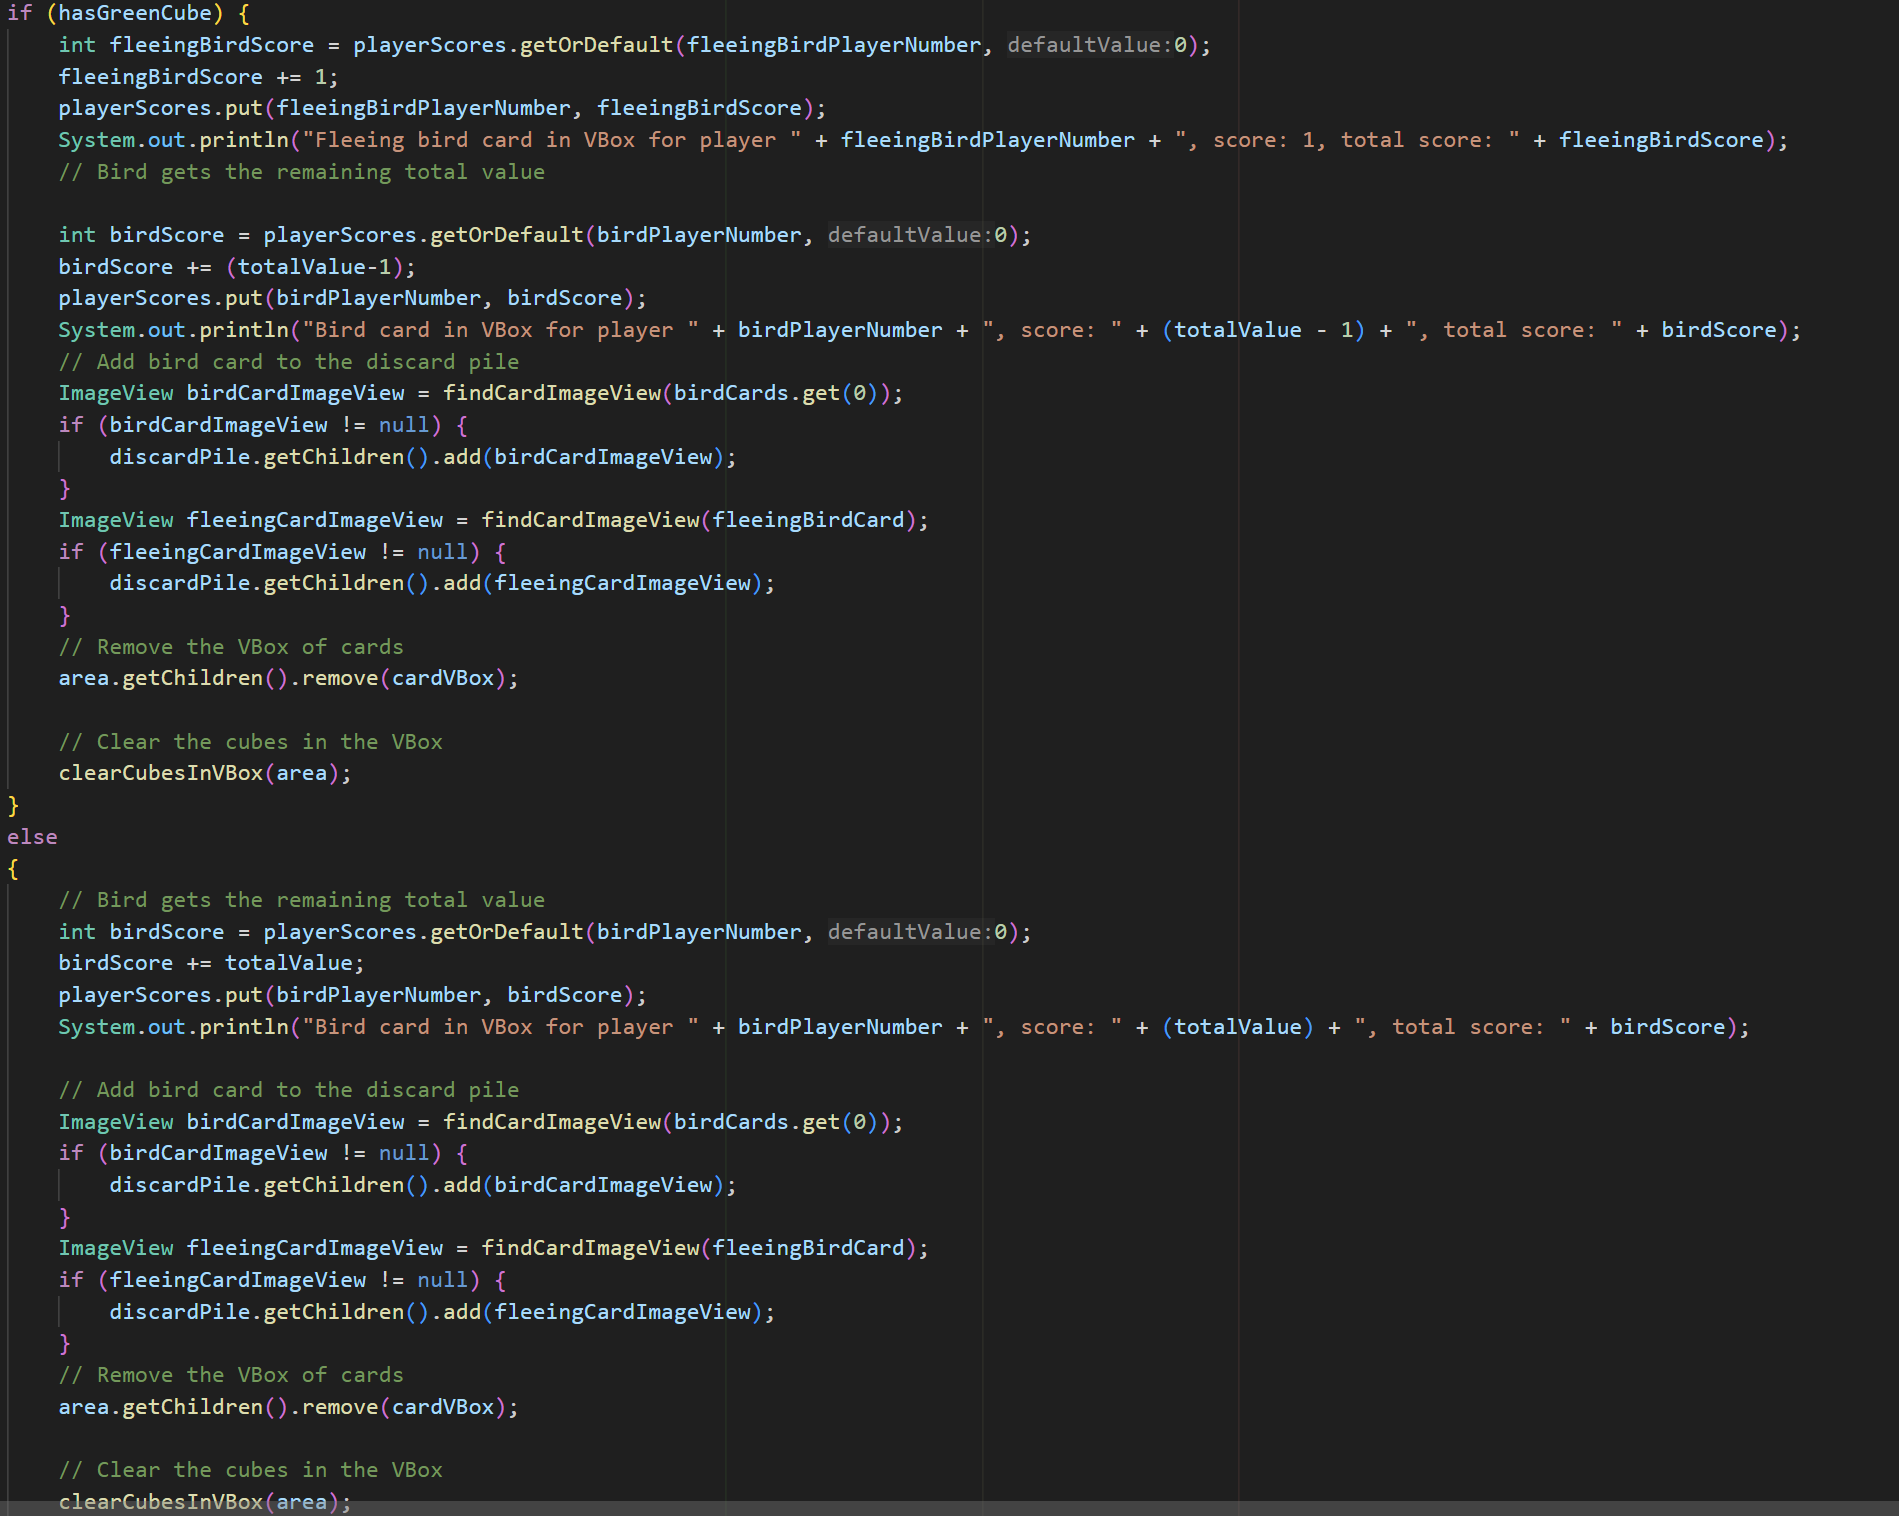
\includegraphics[width=0.48\textwidth]{img/Screenshot 2025-01-14 130307.png} % Adjust the width as needed
        \caption{Case 4}
        \label{fig:case}
    \end{figure}
    \vspace{2cm}
    \item Case 5: When there is 1 bird and 1 fox
    \begin{figure}[h!]
        \centering
        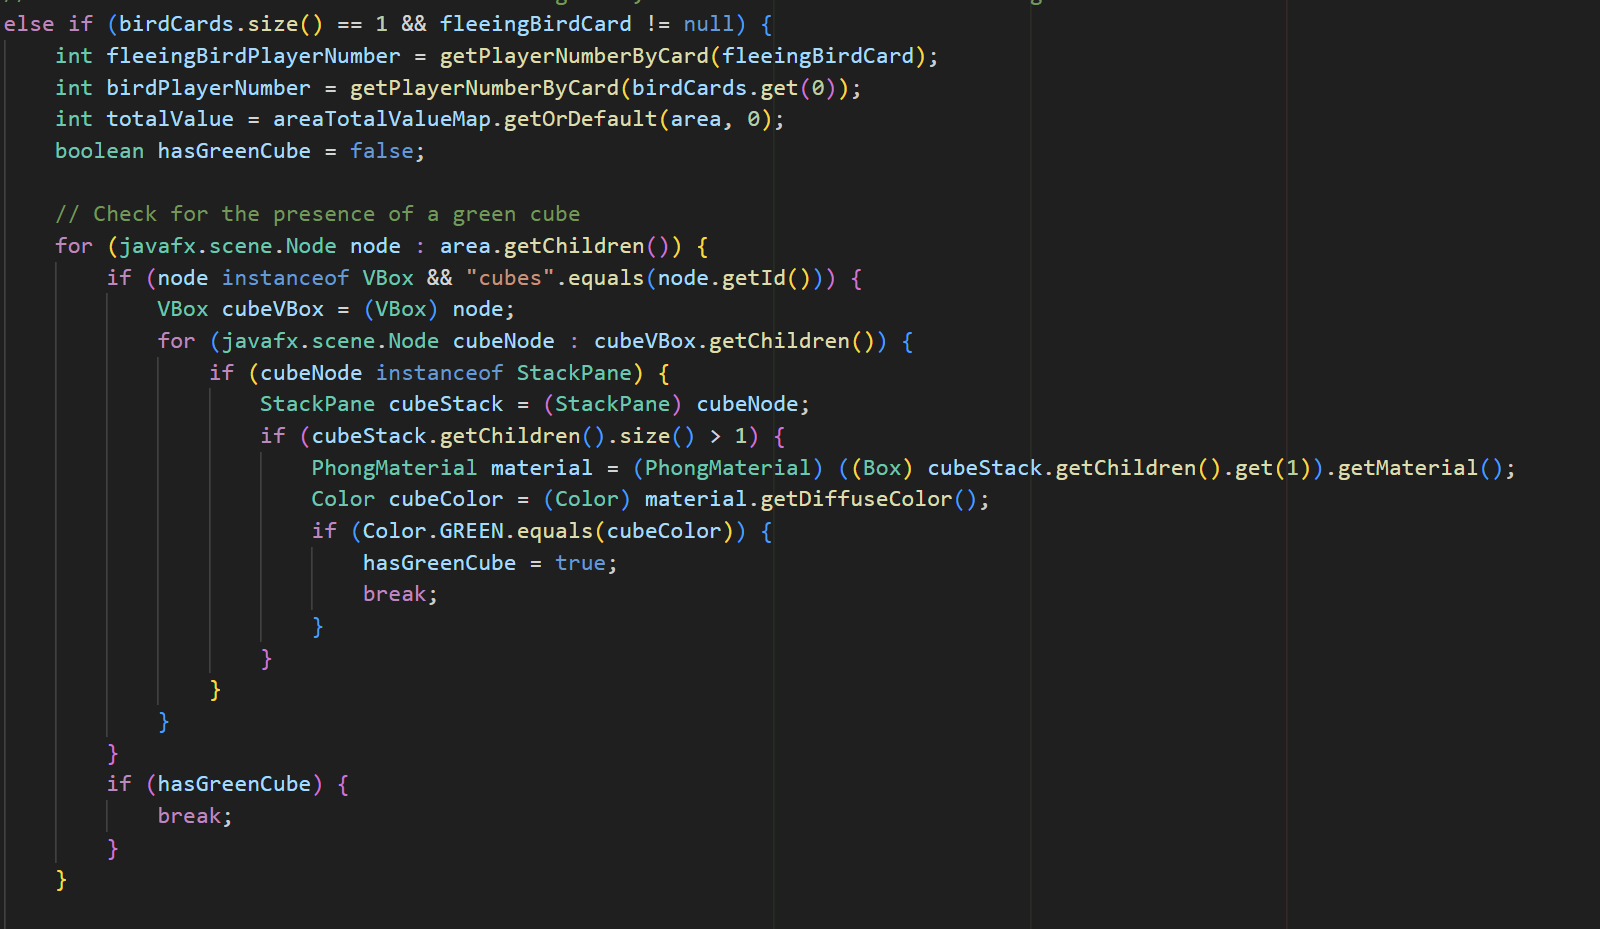
\includegraphics[width=0.47\textwidth]{img/Screenshot 2025-01-14 130113.png} % Adjust the width as needed
        \caption{Case 5}
        \label{fig:case}
    \end{figure}
    \newpage
    \item Case 6: When there is 1 fox and 1 fleeing bird
    \begin{figure}[h!]
        \centering
        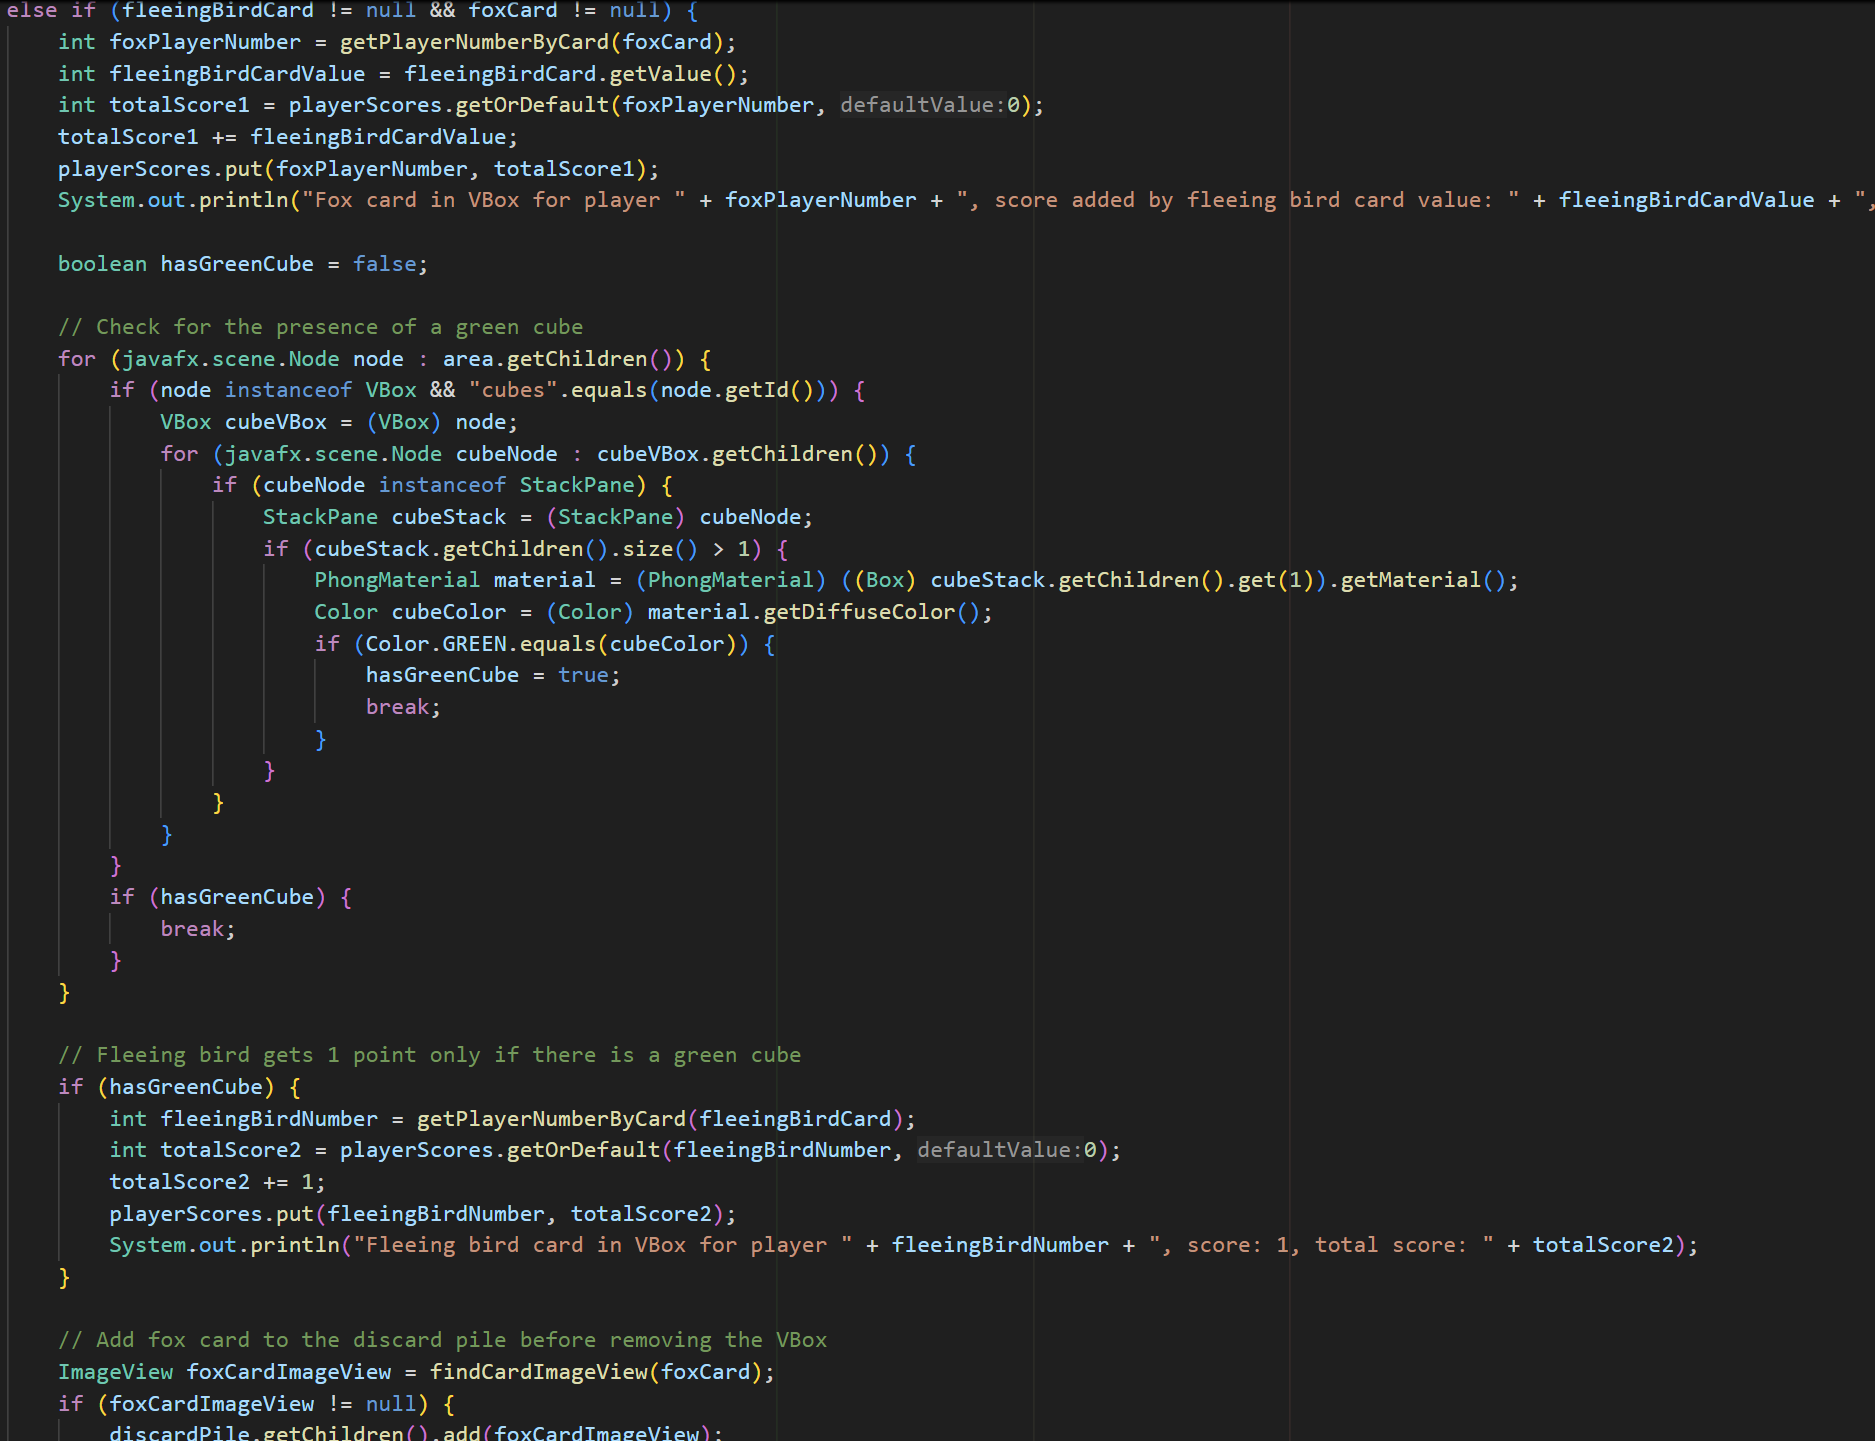
\includegraphics[width=0.47\textwidth]{img/Screenshot 2025-01-14 130523.png} % Adjust the width as needed
        \caption{Case 6}
        \label{fig:case}
    \end{figure}

    \item Method to add delay for bot 
    \begin{figure}[h!]
        \centering
        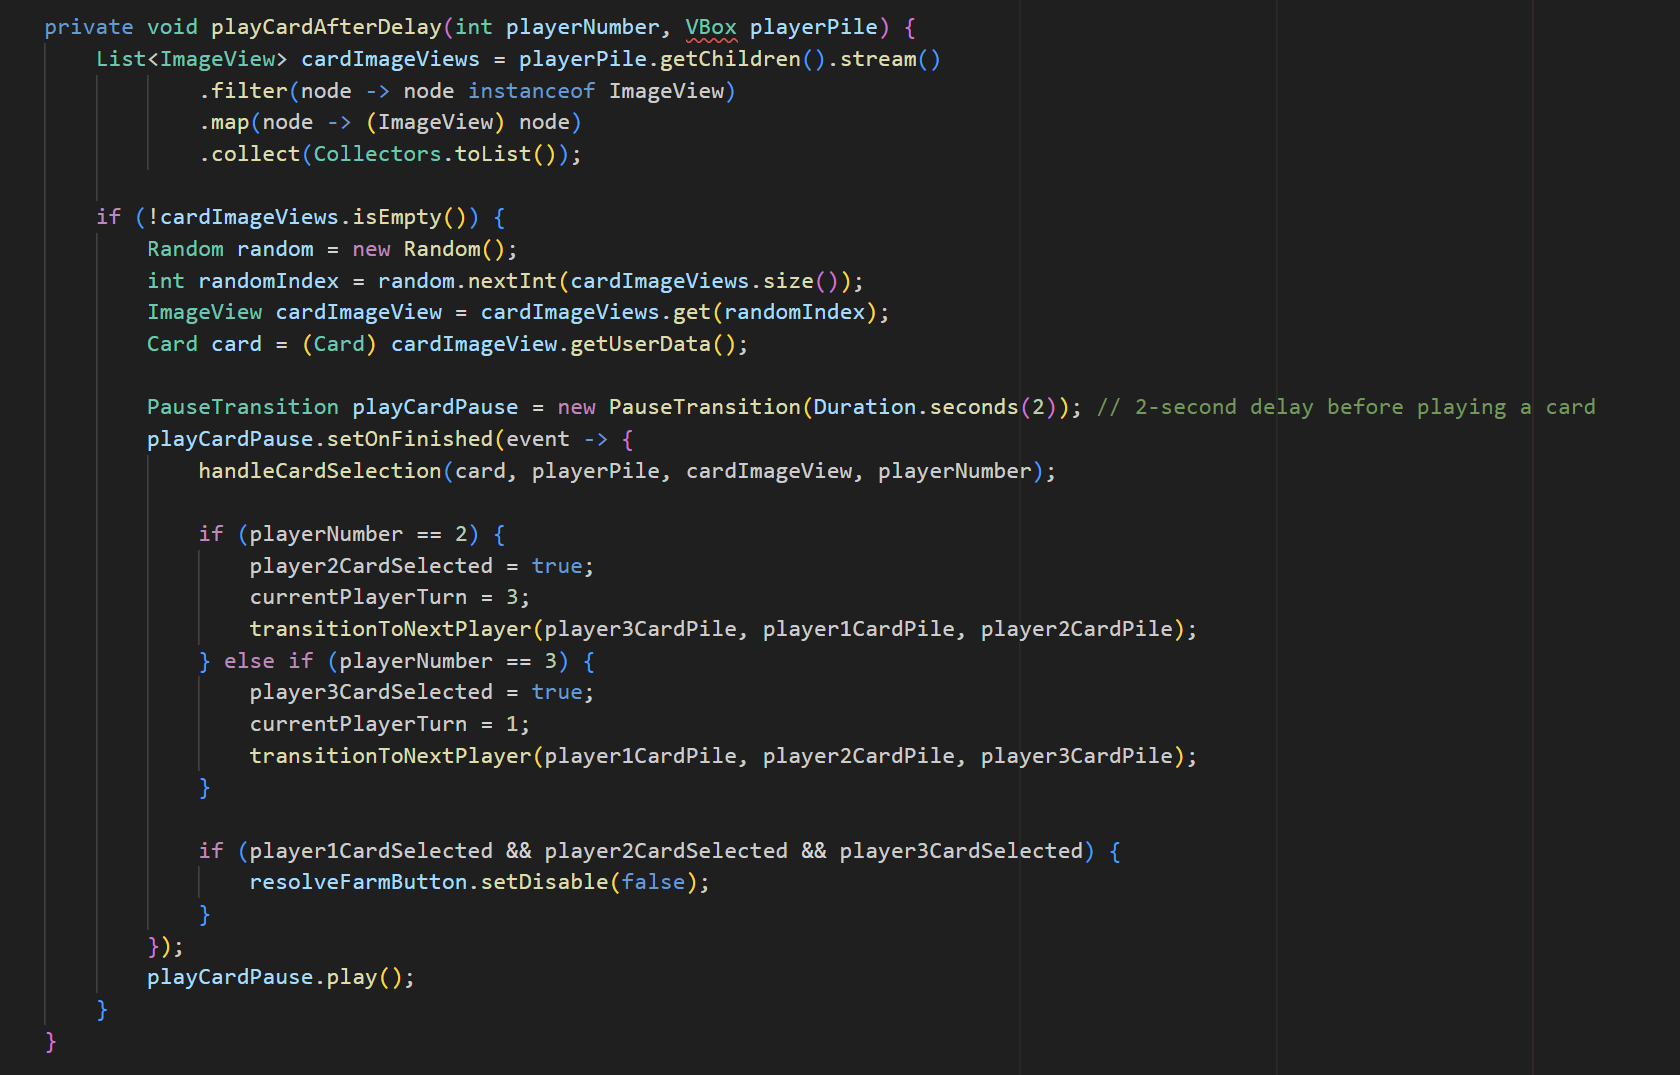
\includegraphics[width=0.47\textwidth]{img/Screenshot 2025-01-17 151752.png} % Adjust the width as needed
        \caption{Add Delay Method for Bot}
        \label{fig:case}
    \end{figure}

    The \textbf{playCardAfterDelay} method manages the delayed selection and playing of a card for a given player in the game. It starts by identifying all \textbf{ImageView} nodes in the player's card pile (\textbf{playerPile}), representing the available cards. If the pile is not empty, it randomly selects one card using a random index. The method retrieves the corresponding Card object from the ImageView. A 2-second delay is introduced with a \textbf{PauseTransition}, after which the selected card is processed via \textbf{handleCardSelection}, which likely manages game-specific actions related to the card.

    The method updates the turn to the next player based on playerNumber (e.g., transitioning from player 2 to 3 or player 3 to 1). If all three players have selected their cards, it enables the resolveFarmButton, allowing further gameplay progression.

    \newpage

    
    \item Method to add random method as a bot for single player.
    The playAutomaticallyForPlayer method automates a player's actions in a card game. It determines the player's card pile (\textbf{player2CardPile} or \textbf{player3CardPile}) based on the provided \textbf{playerNumber}. It collects all the \textbf{ImageView} nodes in the pile, representing the player's cards. If the player has exactly four cards, a 2-second delay is initiated using a \textbf{PauseTransition} before adding a card to the pile with \textbf{addCardsToPlayerPile} and subsequently playing a card with \textbf{playCardAfterDelay}. If the player has fewer than four cards, the method directly triggers the \textbf{playCardAfterDelay} action without delay. This ensures appropriate pacing and card-playing behavior for the player.

    \begin{figure}[h!]
        \centering
        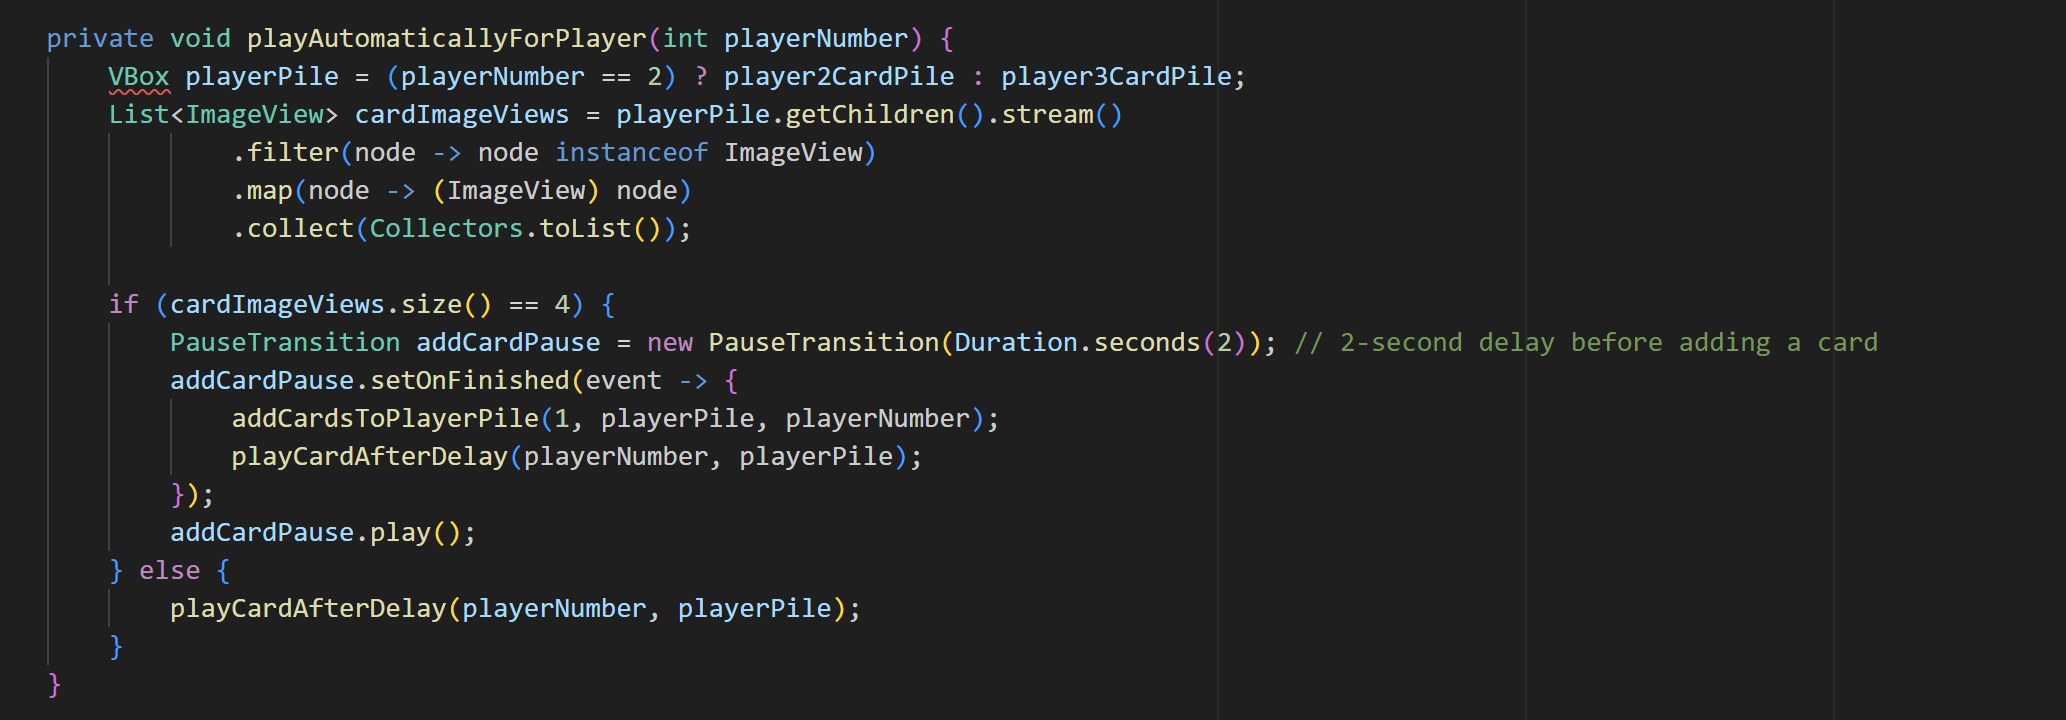
\includegraphics[width=0.47\textwidth]{img/Screenshot 2025-01-17 151307.png} % Adjust the width as needed
        \caption{Automatic Play Method for Bot}
        \label{fig:case}
    \end{figure}
\end{itemize}



These are basic cases that handle basic score rules that are implemented here.
To summarize, these are basic summaries we finalize after writing codes:
\begin{itemize}
    \item When there is only 1 and unique card in the farm:
        \begin{itemize}
            \item If it is a bird or a fleeing bird, it eats all the corns.
            \item If it is a fox, it eats nothing.
        \end{itemize}
    \item When there are 2 cards in a farm
        \begin{itemize}
            \item If there are 2 bird cards, it fights to eat all the corns.
            \item If there are 2 fox cards, it eats nothing.
            \item If there are 1 bird and 1 fox card, fox eats the bird.
            \item if there are 1 bird and 1 fleeing bird card, fleeing bird eat one green corn if there is one in the farm. If else, bird eats all.
            \item IF there are 1 fox and 1 fleeing bird card, fleeing bird eat one green corn if there is one in the farm. Then the fox card eats the fleeing bird. 
        \end{itemize}
    \item When there are 3 cards in a farm
        \begin{itemize}
            \item If there are 3 bird cards, they fight to eat all the corns.
            \item If there are 3 fox cards, they eat nothing.
            \item If there are 2 bird and 1 fox card, the fox eats all the birds.
            \item If there are 2 fox and 1 bird card, the foxes fight to eat the bird.
            \item If there are 2 fox and 1 fleeing bird card, the fleeing bird eat one green corn if there is one in the farm. Then the foxes fight to eat the fleeing bird
            \item If there are 1 fox, 1 bird, and 1 fleeing bird card, the fleeing bird eat one green corn if there is one in the farm. Then the fox eats the bird and fleeing bird.
        \end{itemize}
\end{itemize}

\section{Experimental Results, Statistics Tests, Running Scenarios}
    \begin{figure}[h!]
        \centering
        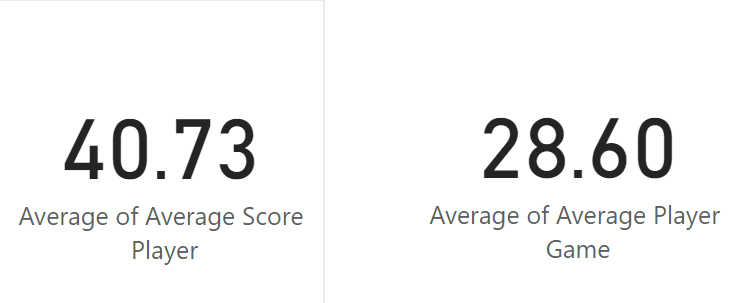
\includegraphics[width=0.47\textwidth]{img/Screenshot 2025-01-18 152405.png} % Adjust the width as needed
        \caption{Average scores of Player on Multiplayer vs. Singleplayer
        }
        \label{fig:case}
    \end{figure}
    
    Based on this numbers, a player choosing Multiplayer mode get an average of approximately 41 points to compete with other players. On the other hand, if player chooses Singleplayer mode, a player can get an average of 28.6 points to compete with 2 bots. The reason behind is that when playing multiplayer, the chance of not challenging each other is low and calculations to get points are easier. However, calculations to get points from bots are more challenging to solve, which results in a lower chance to win the game.


    
    \begin{figure}[h!]
        \centering
        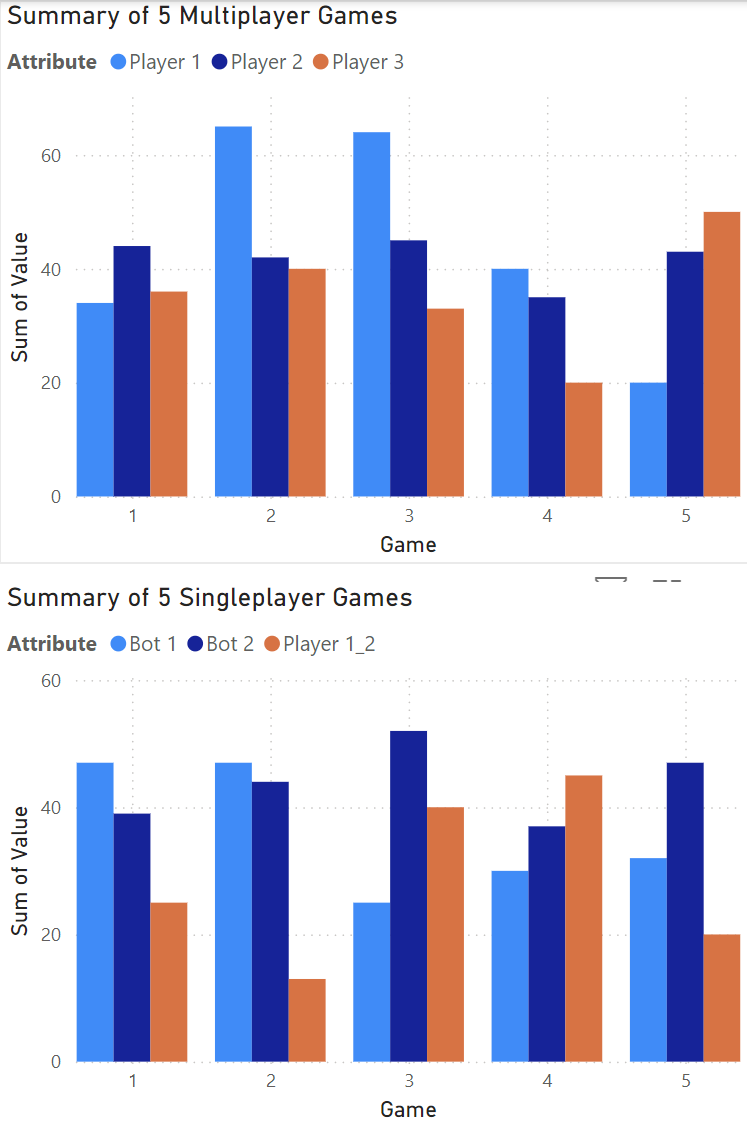
\includegraphics[width=0.45\textwidth]{img/Screenshot 2025-01-18 152209.png} % Adjust the width as needed
        \caption{Score Summary of 5 Games
        }
        \label{fig:case}
    \end{figure}

    \newpage
    In these clustered column charts, there are different trends between 2 charts. On the charts of Multiplayer games, the score of players are mostly higher than 30 points and the probability of chance to win the game of each player is same. On the other hand, the average score of singleplayer is relatively lower, compared to the players in Multiplayer mode, and there are less chances for player to finish the game in 1st place 


    \begin{figure}[h!]
        \centering
        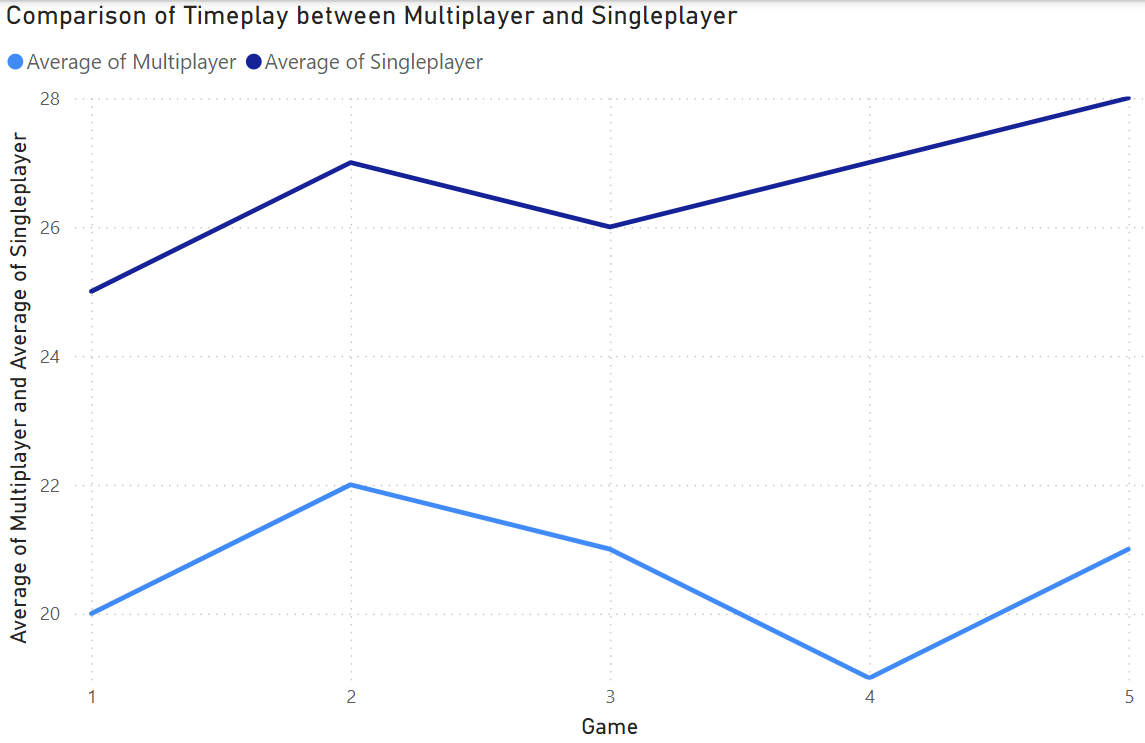
\includegraphics[width=0.47\textwidth]{img/Screenshot 2025-01-18 153925.png} % Adjust the width as needed
        \caption{Timeplay Comparison
        }
        \label{fig:case}
    \end{figure}

    In this line chart, there is a clear difference in the timeplay between Singleplayer and Multiplayer, with the former always higher than 25 minutes and the latter fluctuating around 21 minutes.
    

    

\section{Conclusions and Future Work}

\subsection{How was the teamwork}
The teamwork of my team is great, despite the problem of distance. The members succeeded in overcoming the problem of distance and excellently communicated with other members for a good and beautiful logic and User Interface. Although there are setbacks in the end of December when team had some problems with code, the team managed to finish and documented the report on time and members finished the part of tasks given before deadline of team leader. 
\subsection{What you have learned}
After this project, this is the summary of the knowledge we have achieved:
\begin{itemize}
    \item How to create classes.
    \item How to apply the classes components to the game.
    \item How to write codes clearly and coherently.
    \item How to understand clearly the codes.
    \item How to help readers to understand the codes by adding comments
    \item Seperate the classes of objects to separate files to reduce the total length
    \item How to debug and fix codes.
    \item How to use Scene Builder to create scene for the game.
    \item How to use and fix the FXML files.
    \item How to work with controller to control the scenes and apply transitions between scenes smoothly.
    \item How to add animations to the scenes for animations.
\end{itemize}

\subsection{Ideas for the future development of your application, new algorithms}
In the future, we would love to make improvements and developments to our games. Our features are currently functioning normally; however we have a visual of making the players' card deck become folded when it comes to a player turn and become unfolded when it comes to other players' turn instead of making them invisible at the moment. moreover, we would like to make the transitions of the cards more smoothly and correctly between the card deck and the farms, the farms and the discard deck. There are also animations we would like to make for the introduction scene, game scene and the winner scene, which will make the game more animated and interested for players. 

% \section*{Acknowledgment}

% The preferred spelling of the word ``acknowledgment'' in America is without 
% an ``e'' after the ``g''. Avoid the stilted expression ``one of us (R. B. 
% G.) thanks $\ldots$''. Instead, try ``R. B. G. thanks$\ldots$''. Put sponsor 
% acknowledgments in the unnumbered footnote on the first page.

% \section*{References}

% Please number citations consecutively within brackets \cite{b1}. The 
% sentence punctuation follows the bracket \cite{b2}. Refer simply to the reference 
% number, as in \cite{b3}---do not use ``Ref. \cite{b3}'' or ``reference \cite{b3}'' except at 
% the beginning of a sentence: ``Reference \cite{b3} was the first $\ldots$''

% Number footnotes separately in superscripts. Place the actual footnote at 
% the bottom of the column in which it was cited. Do not put footnotes in the 
% abstract or reference list. Use letters for table footnotes.

% Unless there are six authors or more give all authors' names; do not use 
% ``et al.''. Papers that have not been published, even if they have been 
% submitted for publication, should be cited as ``unpublished'' \cite{b4}. Papers 
% that have been accepted for publication should be cited as ``in press'' \cite{b5}. 
% Capitalize only the first word in a paper title, except for proper nouns and 
% element symbols.

% For papers published in translation journals, please give the English 
% citation first, followed by the original foreign-language citation \cite{b6}.

\begin{thebibliography}{00}
\bibitem{b1} O’Sullivan, Kevin, “Mini Review - Hick Hack in Gackelwack,” Blogspot.com, 2025. Available at: \url{https://tinyurl.com/yv5wnd4v}. Accessed 22 Jan. 2025.
\vspace{1em}

\bibitem{b2} Ubisoft, “UNO by Ubisoft Für Windows,” Softonic, 2023. Available at: \url{https://uno-by-ubisoft.de.softonic.com/?utm_source=bing&utm_medium=paid&utm_campaign=Bing_DE_CH_DSA_Desktop_6524&msclkid=30db4ea61dd11289a7ac29377322bf15}. Accessed 10 Jan. 2025.
\vspace{1em}

\bibitem{b3} D’Arcy, Sean, “Introducing Kahoot!+ Make Learning Awesome for the Entire Family,” Kahoot!, 19 May 2021. Available at: \url{https://kahoot.com/blog/2021/05/19/kahoot-plus-make-learning-awesome-entire-family/}. Accessed 22 Jan. 2025.
\vspace{1em}

\bibitem{b4} GeeksForGeeks, “JavaFX Tutorial,” GeeksforGeeks, 5 Oct. 2021. Available at: \url{https://www.geeksforgeeks.org/javafx-tutorial/}.
\vspace{1em}

\bibitem{b5} “Pick Picknic,” BoardGameGeek, 2020. Available at: \url{https://tinyurl.com/372abme5}. Accessed 22 Jan. 2025.



\end{thebibliography}
% \vspace{12pt}
% \color{red}
% IEEE conference templates contain guidance text for composing and formatting conference papers. Please ensure that all template text is removed from your conference paper prior to submission to the conference. Failure to remove the template text from your paper may result in your paper not being published.

\end{document}
